\documentclass[11pt,reqno]{amsart}

\usepackage{amsmath,amssymb,amsthm}
\usepackage{tikz}
\usetikzlibrary{shapes.geometric, positioning, arrows.meta}
\usepackage{tikz-cd}
\usepackage[hidelinks]{hyperref}

\allowdisplaybreaks
\raggedbottom

\newtheorem{theorem}{Theorem}[section]
\newtheorem{proposition}[theorem]{Proposition}
\newtheorem{lemma}[theorem]{Lemma}
\newtheorem{corollary}[theorem]{Corollary}
\theoremstyle{definition}
\newtheorem{definition}[theorem]{Definition}
\newtheorem{openproblem}[theorem]{Open Problem}
\theoremstyle{remark}
\newtheorem{remark}[theorem]{Remark}

\title[Forced noninjectivity in canonical localization]{Forced noninjectivity and infinite sheet resolution in canonical localization}
\author{Matthew Robert Wesney}
\date{Draft of 2026-07-27}

\begin{document}

\begin{abstract}
Kahn's localization construction for $\psi$-polynomial-like maps produces,
at every renormalization stage, a localized inclusion between marked
covers.  The construction is functorial and preserves immersions; the
sources never assert that it preserves embeddings.  We prove that at every
primitively renormalizable ordinary quadratic-like restriction of a
quadratic polynomial (period $p>1$),
the canonically localized inclusion is \emph{forced} to be noninjective:
the degree budget $2^{p}$ against central degree $2$ produces an excess
component of the pulled central continuum, and a peripheral loop around it
lies outside the source localization subgroup while dying in the target.
The failure is resolved canonically: the localized inclusion factors
uniquely (within the based commuting intermediate-cover class) as a
covering onto an embedded intermediate cover, the fiber of
the covering is a pointed coset set, and this sheet defect is
\emph{infinite}, so no finite sheet enumeration is complete.  In fact
the defect has a canonical group model --- the kernel of the
source-to-target hole-filling homomorphism --- and this kernel
surjects, by peripheral winding numbers, onto $\mathbb Z^{\,2^{p}-2}$,
where $2^{p}-2$ is the elementary degree budget of $F=f^{p}$ against
central degree $2$: canonical localization forgets a hole-filling
kernel with exponentially many independent peripheral directions.  The
novelty claimed here is the winding surjection and the kernel
identification, not the count.  The
resolution propagates through Kahn's exact pullback towers on the full,
unselected complementary-cover locus, and
--- under an explicit strong stage-alignment hypothesis --- to the Kahn--Lyubich
direct-decoration depths, where it forces noninjectivity of the induced
tile lifts and of the glued pseudo-piece immersion.  Finally, the infinite
canonical resolution is incompatible with any whole boundary-extended
Kahn--Lyubich tile factorization satisfying the stated annular-tower
typing: an end-compatible comparison of that type forces a
trivial deck kernel.  Two abstract counterexamples (an exactly certified
Blaschke quotient for Kahn's annulus hypotheses, and a complete abstract
$\psi$-quadratic-like pair with a remote self-collision) show that no
argument from the stated hypotheses alone can restore injectivity.  These
results correct an embedding-preservation route proposed in the author's
research program, not in the sources: they contradict
nothing stated in the published sources, and they do not by themselves
decide any global rigidity statement.  The corrective conclusion is
structural: the canonical localized object at an ordinary primitive
canonical seed is not an
embedded pseudo-piece but an embedded cover \emph{together with} an
infinite coset-valued sheet fibration and its canonical transport.
\end{abstract}

\maketitle
\tableofcontents

%=====================================================================
\section{Introduction}\label{sec:intro}

\subsection{Setting}
Renormalization of quadratic-like maps \cite{DH85}, in the generality
needed for
a priori bounds, takes place in Kahn's category of
$\psi$-polynomial-like maps \cite{KahnPrimitive06}: pairs $(i,f)$ of a
holomorphic \emph{immersion} and a proper branched covering between
disks, with a common connected filled preimage.  A central device of
\cite{KahnPrimitive06}, used again in the Kahn--Lyubich decoration
papers \cite{KLDecorations08,KLPrincipal09}, is \emph{localization}: passing to marked
covers determined by the fundamental group of a neighborhood of a marked
full continuum, so that the dynamics near one small filled Julia set can
be studied with the rest of the cycle removed.  Canonical
renormalization is the dynamical localization of the $p$-th iterate at
the central small filled Julia set $A=K_p$, with the cycle
$B=\mathcal K_p$ removed.

The sources are careful about what this construction preserves.  The
localization functor preserves immersions and branched coverings; the
localized inclusion leg is asserted to be an immersion, never an
embedding; and Kahn notes explicitly that the map which was an embedding
in the quadratic-like setting has become an immersion in the
$\psi$-quadratic-like setting.  We are not aware of any statement in
the literature determining whether this caution is necessary at the
canonical stages themselves --- whether the canonically localized
inclusion might in fact be injective, so that localization could be
treated as embedding-preserving in arguments that need a globally
embedded local model.  Section~\ref{subsec:literature} records what we
did examine and what the closest published anticipation is.

\subsection{Main results}
We show that the caution is necessary in the strongest possible sense:
noninjectivity is not merely possible but \emph{forced}, at every
ordinary primitive canonical seed, and the failure carries a canonical
infinite structure.

Throughout, $f\colon U^{1}\to U^{0}$ is an ordinary quadratic-like
restriction of a quadratic polynomial, primitively renormalizable of
period $p>1$; $F=f^{p}\colon U^{p}\to U^{0}$; $A=K_{p}$ is the central
small filled Julia set and $B=\mathcal K_{p}$ its cycle;
$T'=(U^{p}\setminus F^{-1}B)\cup A$ and $T=(U^{0}\setminus B)\cup A$ are
the marked surfaces of Kahn's canonical localization, with localization
subgroups $H_{s}\le\pi_{1}(T'\setminus A)$ and
$H_{t}\le\pi_{1}(T\setminus A)$, localization covers
$\widehat\Omega_{s}$ and $\widehat\Omega_{t}$ of the complementary
surfaces $\Omega_{s}=T'\setminus A$ and $\Omega_{t}=T\setminus A$,
complement-cover lift
$\widehat a\colon\widehat\Omega_{s}\to\widehat\Omega_{t}$, and localized
inclusion $\widehat\imath\colon T'_{A}\to T_{A}$.

\begin{theorem}[Forced noninjectivity; Theorem~\ref{thm:forced-collision}]
\label{thm:A}
At every ordinary primitive canonical seed of period $p>1$, the
canonically localized inclusion $\widehat\imath$ is not injective.
Explicitly, there are an excess component $X\neq A$ of $F^{-1}(A)$ and a
based loop $\gamma\subset U^{p}\setminus F^{-1}B$ with
$[\gamma]\notin H_{s}$ and $(i^{p})_{*}[\gamma]=1\in H_{t}$, and the
lift of $\gamma$ has distinct endpoints identified by
$\widehat\imath$.
\end{theorem}

\begin{theorem}[Canonical resolution; Theorems~\ref{thm:sheet-resolution}
and~\ref{thm:unique-intermediate}]\label{thm:B}
The complement-cover lift $\widehat a$ of $i^{p}$ factors exactly as
$\widehat a=e\circ q$, where
$q\colon\widehat\Omega_{s}\to P_{K}$ is a surjective covering onto the
basepoint component $P_{K}$ of the corresponding pullback cover and
$e\colon P_{K}\hookrightarrow\widehat\Omega_{t}$ is a topological
embedding.  Every point collision of $\widehat\imath$ lies in the
complement-cover part, where $\widehat\imath$ agrees with $\widehat a$,
and is a sheet identification of $q$; the
based fiber of $q$ is the pointed coset set $K/H_{s}$ with
$K=(i^{p})_{*}^{-1}(H_{t})$ the reflected subgroup; and $P_{K}$ is the
unique connected intermediate cover, in the based commuting comparison
class of Theorem~\ref{thm:unique-intermediate}, on which the remaining
leg embeds.  No extension of the factorization across the filled
completion is asserted.
\end{theorem}

\begin{remark}[The structural shape of Theorem~\ref{thm:B} is not new]
\label{rem:covering-embedding-prior}
The shape asserted by Theorem~\ref{thm:B} --- an immersion that is a
covering onto an embedded image away from a proper compactum --- is
already an axiomatised notion in the recent literature.
Dudko--Luo--Lyubich \cite[\S2.1]{DLL25} call an immersion
$\iota\colon A\to B$ a \emph{covering embedding rel $S\subset B$} when
$S$ is $\iota$-proper and $\iota$ restricted to
$A\setminus\iota^{-1}(S)$ is a covering onto its image, and they impose
this as Items (V)--(VI) of their $\psi$-ql Siegel definition.  Their
setting is different (Siegel rather than primitive) and, decisively,
the property is \emph{imposed} there as part of a definition.  The
contribution of Theorem~\ref{thm:B} is not the notion but its
canonical derivation at the seed: the factorization is produced,
its intermediate factor is shown to be unique in a stated comparison
class, and its fiber is identified with an explicit dynamical coset
set.
\end{remark}

\begin{theorem}[Infinite sheet defect;
Corollary~\ref{cor:infinite-defect}]\label{thm:C}
At every ordinary primitive canonical seed, $[K:H_{s}]=\infty$:
the cosets $[\gamma]^{n}H_{s}$ are pairwise distinct.  Consequently
every non-singleton fiber of $\widehat\imath$ (equivalently, every
fiber over the embedded resolved complement component) is infinite and
no finite raw
sheet enumeration of the canonical localization is complete.
\end{theorem}

\begin{theorem}[Kernel normal form;
Theorem~\ref{thm:kernel-normal-form}]\label{thm:Cprime}
At every ordinary primitive canonical seed, with the shared local
neighborhood and based subgroup representatives of
Definition~\ref{def:shared-neighborhood}, the hole-filling
homomorphism $a_{*}=(i^{p})_{*}$ restricts to an isomorphism
$H_{s}\to H_{t}$, and the reflected subgroup splits as
$K=N_{\mathrm{fill}}\rtimes H_{s}$ with
$N_{\mathrm{fill}}=\ker a_{*}$.  Consequently $n\mapsto nH_{s}$ is a
canonical pointed bijection $N_{\mathrm{fill}}\to K/H_{s}$: the sheet
fiber carries a canonical group model, and canonical localization
forgets exactly the kernel of the source-to-target hole-filling map.
\end{theorem}

\begin{theorem}[Exact excess count and exponential defect;
Theorem~\ref{thm:excess-count},
Corollary~\ref{cor:exponential-defect}]\label{thm:Cpp}
At every ordinary primitive canonical seed of period $p>1$ the central
preimage decomposes as
$F^{-1}(A)=A\sqcup X_{1}\sqcup\cdots\sqcup X_{2^{p}-2}$, where each
excess component $X_{j}$ is a full continuum disjoint from $B$ mapped
homeomorphically onto $A$ by $F$.  The peripheral winding vector about
the excess components is a surjective homomorphism
$N_{\mathrm{fill}}\twoheadrightarrow\mathbb Z^{\,2^{p}-2}$; hence
$\operatorname{rank}H_{1}(N_{\mathrm{fill}};\mathbb Z)\ge 2^{p}-2$,
and the forgotten sheet fiber carries at least $2^{p}-2$ independent
peripheral winding coordinates.
\end{theorem}

Two calibrations of Theorem~\ref{thm:Cpp}.  The count $2^{p}-2$ is an
elementary degree budget --- $\deg F=2^{p}$, the only critical point of
$F$ whose critical value lies in $A$ is the origin, so every other
component of $F^{-1}(A)$ is univalent --- and we claim no novelty for
it; the existence of non-central components is in any case structurally
built into the hypothesis of the Kahn--Lyubich Covering Lemma
(\cite[\S4]{KLDecorations08}: $A$ is a component of $f^{-1}(B)$ with
big degree $D$ and local degree $d$, and $D>d$ forces further
components).  What is claimed is the peripheral-winding surjection
$N_{\mathrm{fill}}\twoheadrightarrow\mathbb Z^{\,2^{p}-2}$ and the
resulting rank bound.  Likewise, the abstract covering-space
factorization is standard; the contribution is the identification of
the actual dynamical subgroup defect and its canonical kernel model,
not the invention of intermediate covers.

\begin{theorem}[Exact propagation; Proposition~\ref{prop:base-change},
Corollary~\ref{cor:kahn-tower}, Theorem~\ref{thm:propagation}]\label{thm:D}
The factorization and its fiber data are preserved by every full,
unselected exact Kahn equalizer on the complementary-cover locus, hence
by every depth of Kahn's pullback iteration of the same seed.  Under
the strong stage-alignment hypothesis
(Definition~\ref{def:strong-alignment}), the
collision transports to the exact decoration depths
$m=\nu q+1$, $n=(\nu-1)q+1$, where it forces noninjectivity of the
Kahn--Lyubich ambient annulus arrow, of every compatible full
universal-cover tile lift, and of the full glued pseudo-piece
immersion.
\end{theorem}

\begin{theorem}[No aligned annular realization of the canonical
infinite resolution is a whole KL tile;
Theorem~\ref{thm:whole-tile-no-go},
Corollary~\ref{cor:canonical-not-whole-tile}]\label{thm:E}
Whenever the canonical resolved factorization restricts, at an aligned
stage, to a covering/embedding factorization of a degree-one immersion
of finite-modulus annuli, the full annular-tower typing of
Definition~\ref{def:canonical-resolved-system} is automatic
(Theorem~\ref{thm:annular-normal-form}), and no end-compatible
whole-tile comparison square can identify the
canonical resolved factorization with a complete boundary-extended
Kahn--Lyubich tile factorization carrying the two source-locked
infinitely-wrapping vertices: any such comparison forces the deck
kernel to be trivial, while the canonical resolution has infinite
sheet defect.  The statement is conditional only on the aligned-stage
annular factorization; the typing is derived, not assumed.
\end{theorem}

Two abstract counterexamples calibrate the main theorems.  A degree-one
annular immersion satisfying all stated hypotheses of Kahn's annulus
lemma can fail to be injective (Theorem~\ref{thm:annulus-nogo}; an
exactly certified Blaschke quotient), and the complete abstract
$\psi$-quadratic-like axioms admit a pair whose immersion has an
explicit remote self-collision (Theorem~\ref{thm:psiql-nogo}).  Thus no
proof from the stated hypotheses alone --- degree, immersion,
properness of the companion branch, common connected inverse --- can
restore global injectivity; the forced collision of
Theorem~\ref{thm:A} is a fact about the actual dynamical construction,
established by the actual excess-component geometry.

\subsection{Relation to the literature}
\label{subsec:literature}
Because the results above are stated against two specific sources, we
record what was examined, what the closest published anticipation is,
and how much of the argument is short once one knows to look for it.

\emph{What the primary sources assert.}  Kahn's localization functor is
asserted to preserve immersions and branched coverings and nothing more
(\cite[\S\S7.4.1--7.4.2, pp.~43--45]{KahnPrimitive06}); at the
quadratic-like stage the arrow $i$ is literally the inclusion of nested
domains, and a footnote announces that in the $\psi$-quadratic-like
sections it will be replaced by an immersion
(\cite[\S6, p.~31 and footnote 15]{KahnPrimitive06}); and the setup
ingredient of the present argument is already visible in the source, since
\cite[\S6.1, pp.~31--32]{KahnPrimitive06} exhibits the hole-filling leg
$U^{n+1}\setminus f^{-1}\mathcal K\subset U^{n+1}\setminus\mathcal K$ as
one side of a triangle the text explicitly calls non-commutative, and
controls passage along it quantitatively via Property~D.  On the
Kahn--Lyubich side the pseudo-piece inclusion arrow is never upgraded
beyond an immersion \cite[\S3.2.2, Lemma~3.4]{KLDecorations08}.

\emph{The closest published anticipation.}  It is by the source authors
themselves, and it deserves to be in the introduction rather than in an
appendix.  In the proof of \cite[\S3.2.2, Lemma~3.4(ii), p.~68 of the
journal pagination]{KLDecorations08}, for puzzle pieces $Y\subset Z$ the
components $Y_{i}$ are embedded into components $Z_{j(i)}$, and the
component index map $j=j(i)$ is described as ``surjective but not
necessarily injective''.  That is the collapsing-of-components
mechanism, in print, since 2008.  Theorem~\ref{thm:A} differs from it in
three specific ways.
\begin{enumerate}
\item[(1)] It is a \emph{forcing} statement, not a possibility
  statement: at every ordinary primitive canonical seed the collision
  must occur, whereas ``not necessarily injective'' asserts only that
  injectivity is not guaranteed.
\item[(2)] It concerns the \emph{glued immersion}, not the component
  index map $j$.  Noninjectivity of $j$ does not imply noninjectivity of
  the glued map: distinct universal-cover tiles can occupy disjoint
  sheets over one target tile, so a two-to-one $j$ is compatible with
  an injective glued arrow.
\item[(3)] It concerns Kahn's localization functor at a canonical
  \emph{seed}, not Kahn--Lyubich pseudo-puzzle tiles at an arbitrary
  puzzle depth.
\end{enumerate}

\emph{On difficulty.}  We do not present Theorem~\ref{thm:A} as hard.
In Kahn's own path model of the canonical localization
(\cite[\S7.4.5, pp.~46--47]{KahnPrimitive06}), where the source class
space is formed rel $f^{-p}(K_{p})$ and the target rel $\mathcal K_{p}$
and the source proves only the forward direction of path equivalence,
the failure of injectivity is a short argument once one thinks to look
for it: a loop around an excess component of
$f^{-p}(K_{p})\setminus\mathcal K_{p}$ is nontrivial in the source
class space and trivial in the target.  We are not aware of anyone
having recorded it, and the substance of this paper lies in what
follows from it --- the kernel normal form, the infinitude
$[K:H_{s}]=\infty$, the rank-$(2^{p}-2)$ winding surjection, and the
propagation and no-go results.

\emph{Post-2008 work on this machinery.}  We examined the papers that
actually use the $\psi$-ql/localization apparatus and found no
statement of, and nothing contradicting, Theorem~\ref{thm:A}.  The most
recent restatement of the construction is by two of the three source
authors: Kahn--Kapiamba--Lyubich \cite[\S\S2.2--2.3]{KKL26} recall
localization via subsurface covers and renormalization, and still
assert only that the pair $(f^{n},\iota^{n})$ \emph{lifts} to a
$\psi$-ql map --- no embedding, injectivity, or sheet statement.  The
same holds in \cite{KLElephant26}, where $\iota$ is used on
complements with no injectivity claim; in the Dudko--Lyubich
renormalization papers \cite{DL22,DL23}; in the Siegel variation
\cite{DLL25}, whose \S2.1 axiomatises the covering-embedding shape
discussed in Remark~\ref{rem:covering-embedding-prior}; in
\cite{CS15}; and in \cite{BLOT22}.  Dudko's survey \cite{Dudko25}
does not treat the localization functor at this level of detail.  We
make no claim of an exhaustive search: the negative result rests on the
citation graphs of the two sources together with targeted full-text
checks, not on a complete bibliographic sweep.

\subsection{What these results do and do not assert}
\label{subsec:scope}
Three boundaries govern everything below and are restated where they
apply.

\emph{First}, the results contradict nothing stated in the published
sources \cite{KahnPrimitive06} and \cite{KLDecorations08}; the exact
identification points on which this interface rests are listed in
Section~\ref{sec:verification}.  Those sources
assert immersion preservation, a homeomorphism on filled and marked
sets, an embedded inner collar, and the forward direction of path
equivalence --- never a global embedding of the localized inclusion.
In particular the embedded inner collar of
\cite[Theorem~7.3, p.~37]{KahnPrimitive06} and
\cite[Lemma~3.1, p.~10]{KLDecorations08} is \emph{not} in tension with
Theorem~\ref{thm:A}: the forced collision is located outside the
collar, on a peripheral loop around an excess component in the outer
part of the source, as spelled out in
Remark~\ref{rem:collar-compat}.  What is refuted is a proposed
\emph{extension} of the sources: any argument treating canonical
localization as embedding-preserving.
Appendix~\ref{sec:disclosures} documents where the sources themselves
demote the inclusion to an immersion.

\emph{Second}, the direct-decoration consequences in
Theorem~\ref{thm:D} are conditional on the strong stage-alignment
hypothesis (Definition~\ref{def:strong-alignment}) for the same
canonical seed; the alignment and realization
quantifiers are stated exactly in Proposition~\ref{prop:realization},
and no source-locked parameter realization is claimed.  As
Remark~\ref{rem:alignment-is-seed-identification} explains, that
hypothesis is not a comparison of two constructions --- the
Kahn--Lyubich ambient arrow is literally an iterate of Kahn's
equalizer tower --- but an identification of two \emph{seeds}: on the
reading this paper intends, in which the Kahn--Lyubich puzzle
machinery is run over the canonical seed itself, the identifications
are the identity and Theorem~\ref{thm:D} is unconditional; it is the
distinct-seed reading that remains open.

\emph{Third}, the results are corrective, not constructive, with
respect to any global program: they show that the full embedded
pseudo-piece cannot be the universal carrier invariant, and that a
valid replacement must retain the coset-valued sheet fibration and its
transport, or synchronize the removed obstacle packet.  They do not by
themselves prove or refute any rigidity, a~priori bounds, or local
connectivity statement, and we make no claim in that direction.

\subsection{Organization}
Section~\ref{sec:background} fixes the $\psi$-polynomial-like
background and the localization construction.  All citations into the
two primary sources are given by published section, statement number
and page; the SHA-256--locked \TeX{} archives on which the paraphrases
were originally prepared are retained only as a provenance concordance
in Appendix~\ref{app:sourcelock}.
Section~\ref{sec:criteria} develops the criterion layer: the
subgroup-reflection criterion and peripheral isolation of pulled full
continua.  Section~\ref{sec:forced} proves
Theorem~\ref{thm:A}; Section~\ref{sec:resolution} proves
Theorems~\ref{thm:B} and~\ref{thm:C} and constructs the sheet-transport
groupoid; Section~\ref{sec:enlargement} gives the exact coset tests for
enlargement.  Section~\ref{sec:kernel} proves
Theorems~\ref{thm:Cprime} and~\ref{thm:Cpp}: the kernel normal form,
the exact excess count, and the exponential winding defect of the
hole-filling kernel.  Section~\ref{sec:basechange} proves the
base-change half
of Theorem~\ref{thm:D}; Section~\ref{sec:tiles} transports the
collision to tiles and pseudo-pieces; Section~\ref{sec:wholetile}
proves Theorem~\ref{thm:E}.  Section~\ref{sec:seedvsbold} separates the
ordinary canonical seed from a general bold Kahn--Lyubich stage.
Section~\ref{sec:changes} states what these results change in
localization arguments.  Section~\ref{sec:verification} records the
outcome of the source check on the identifications on which the
interface with the sources rests, together with the exact scope of the
machine-checked certificates.  Appendix~\ref{sec:disclosures} collects
the annulus immersion lemma and the sources' immersion disclosures;
Appendix~\ref{sec:abstract} gives the
two abstract counterexamples.  Appendix~\ref{app:certificates} records
the certificate conventions; Appendix~\ref{app:sourcelock} records the
source-lock data.

\subsection*{Provenance and verification disclosure}
This paper was prepared with extensive machine assistance, both in the
research phase and in drafting, within a source-locked, machine-audited
research framework; the supporting dependency ledger and validation
scripts are available with the manuscript sources.  The
machine-verified content is strictly delimited (exact rational
certificates for Appendix~\ref{sec:abstract}; source-lock hashes;
arithmetic and routing checks) and is described in
Section~\ref{sec:verification}.  We stand behind the unconditional
core of the paper --- the forced collision, the canonical resolution,
the kernel normal form, and the exact excess count.  The Kahn-side
identifications on which that core rests have now been checked against
the published sources and are recorded as confirmed, with their
published loci, in Section~\ref{sec:verification}; specialist
confirmation is invited but the checks are no longer unperformed.  The
Kahn--Lyubich consequences are stated as precise implications under
the strong stage-alignment hypothesis
(Definition~\ref{def:strong-alignment}), whose real content ---
identifying two seeds, not two constructions --- is analysed in
Remark~\ref{rem:alignment-is-seed-identification}.  On the reading
this paper intends, in which the Kahn--Lyubich puzzle machinery is run
over the canonical seed itself, those consequences are unconditional;
supplying the identifications for a \emph{different} seed is the one
source-side proposition that remains open.

%=====================================================================
\section{Background: $\psi$-polynomial-like maps and localization}
\label{sec:background}

This section fixes definitions and records, in paraphrase, exactly what
the published sources provide.  Citations read
``Kahn~I, \S X / Theorem~N, p.~P'' for
\cite{KahnPrimitive06} in the numbering of arXiv:math/0609045v3
(28 December 2023, 63 pp.), and ``KL~II, Lemma~N, p.~P'' for
\cite{KLDecorations08} in the numbering of
Ann.\ Sci.\ \'Ec.\ Norm.\ Sup\'er.\ (4) \textbf{41} (2008) 57--84 and
of the identically sectioned arXiv:math/0609046v2.  The SHA-256--locked
\TeX{} archives from which the paraphrases were prepared, and their
concordance to these published loci, are recorded in
Appendix~\ref{app:sourcelock}.

\emph{Path convention.}  For paths $\alpha,\beta$ with
$\alpha(1)=\beta(0)$, the concatenation $\alpha*\beta$ traverses
$\alpha$ first.  All displayed loop products below use this
convention.

% ---- begin F:notation ----
%% ================= Cluster F: notation and conventions =================
%% Kahn source background for the background section and the
%% exact-identification subsection.  Assumes amsmath, amssymb, amsthm;
%% theorem/lemma/proposition/definition/remark environments are assumed
%% declared in the main preamble.

\providecommand{\C}{\mathbb{C}}
\providecommand{\D}{\mathbb{D}}
\providecommand{\T}{\mathbb{T}}
\providecommand{\N}{\mathbb{N}}
\providecommand{\Z}{\mathbb{Z}}
\providecommand{\Ann}{\mathbb{A}}          % round annulus \Ann(r,R)
\providecommand{\BU}{\mathbf{U}}           % ambient disk (psi-ql source side)
\providecommand{\BV}{\mathbf{V}}           % ambient disk of a localization
\providecommand{\sm}{\setminus}
\providecommand{\KK}{\mathcal{K}}          % cycle of small filled Julia sets
\providecommand{\Mod}{\operatorname{mod}}        % conformal modulus
\providecommand{\Ind}{\operatorname{Ind}}        % winding number

%% Conventions (all traceable to the locked Kahn/KL sources):
%%  * \T_r=\{|z|=r\}, \T=\T_1, \Ann(r,R)=\{r<|z|<R\}
%%    [Kahn I, intro.tex, ll. 249-252].
%%  * ``FJ-set'': compact, connected, full, more than one point
%%    [Kahn I, intro.tex, ll. 254-256].
%%  * A psi-polynomial-like (psi-pl) map is a pair (i,f)\colon\BU'\to\BU
%%    as in the Definitions block; K is its filled Julia set and
%%    K'=i^{-1}(K)=f^{-1}(K) [Kahn I, psiql2.tex, ll. 16-41].
%%  * (S_A,\widehat A) and \pi_{S,A} denote Kahn's localization of a
%%    marked Riemann surface (S,A) [psiql2.tex, ll. 456-498].
%%  * Canonical seed: f\colon U^1\to U^0 a quadratic-like restriction of
%%    a quadratic polynomial, primitively renormalizable of period p>1;
%%    U^r=f^{-r}(U^0); F=f^p\colon U^p\to U^0; physical inclusion
%%    a=i^p\colon U^p\hookrightarrow U^0; A=K_p; B=\KK_p
%%    [Kahn I, pullback.tex ll. 2-7; intro.tex ll. 22-47;
%%     psiql2.tex ll. 549-558].
%%  * Complementary marked surfaces of the canonical localization:
%%    T=(U^0\sm B)\cup A, T'=(U^p\sm F^{-1}B)\cup A
%%    [psiql2.tex, ll. 528-529]; complementary annulus bases
%%    \Omega_s=U^p\sm F^{-1}B, \Omega_t=U^0\sm B.
%%  * H_s\le\pi_1(\Omega_s,z_*), H_t\le\pi_1(\Omega_t,z_*): based
%%    localization subgroups realized by local neighborhoods of A
%%    (Definitions block; local notes, forced-collision Sec. 5).
%%  * Pullback tower: (i_n,f_n)\colon(\BU^{n+1},K^{n+1})\to(\BU^n,K^n),
%%    with i_n\circ f_{n+1}=f_n\circ i_{n+1}
%%    [psiql2.tex, ll. 350-416].
%%  * KL II direct-decoration data: satellite period q, escape depth
%%    \nu; P=Y^{(\nu-1)q+1}; Q_L,Q_R the univalent f^q-pullbacks of P
%%    of depth \nu q+1 [KL II, kingdom.tex, ll. 116-137].
% ---- end F:notation ----
% ---- begin F:definitions ----
\begin{definition}[FJ-set; Kahn I, \S1.5]\label{def:fjset}
A set \(K\subset\C\) (or in a Riemann-surface disk) is an \emph{FJ-set}
(``filled-Julia-like set'') if it is compact, connected, full, and has
more than one point.
\end{definition}

\begin{definition}[\(\psi\)-polynomial-like map; Kahn I, Definition 7.1, p.~36]\label{def:psipl}
A \emph{\(\psi\)-polynomial-like map} (with connected Julia set) of degree
\(d\) is a pair of holomorphic maps \((i,f)\colon\BU'\to\BU\) together
with an FJ-set \(K\subset\BU\) such that:
\begin{enumerate}
\item \(\BU'\) and \(\BU\) are disks;
\item \(i\) is an immersion;
\item \(f\) is a proper branched covering of degree \(d\);
\item \(i^{-1}(K)=f^{-1}(K)=:K'\); and
\item \(K'\) is connected.
\end{enumerate}
\(K\) is the \emph{filled Julia set} of \((i,f)\).  The source records
(Definition~7.1 and the remark following it, p.~36; \S7.3.2, p.~42): \(K'\) is again an FJ-set; connectivity of \(K'\)
is equivalent to all branch values of \(f\) lying in \(K\); the set
\(K\) is determined by the pair \((i,f)\); and
\(i\colon K'\to K\) is a bijection (used later as a homeomorphism).
A degree-two \(\psi\)-polynomial-like map is \emph{\(\psi\)-quadratic-like}.
\end{definition}

\begin{definition}[marked surfaces, local pairs, local covers; Kahn I, \S7.4.1, p.~44]\label{def:local}
A \emph{marked Riemann surface} is a pair \((S,A)\) with \(S\) a Riemann
surface and \(A\subset S\) compact, connected, and full (no component of
\(S\sm A\) has compact closure in \(S\)).  A \emph{morphism}
\(g\colon(S,A)\to(T,B)\) is a holomorphic map with \(A=g^{-1}(B)\).
The pair \((S,A)\) is \emph{local} if every component of \(S\sm A\) is
an annulus; in that case \(S\) deformation-retracts into any
neighborhood of \(A\).  For every \((S,A)\) and every neighborhood
\(V\supset A\) there is a subsurface \(U\subset V\) containing \(A\)
with \((U,A)\) local; such \(U\) is a \emph{local neighborhood} of
\(A\).  A morphism \(g\colon(S,A)\to(T,B)\) is a \emph{local cover} if
\(g\colon A\to B\) is a bijection and \(g\colon S\sm A\to T\sm B\) is a
covering map.
\end{definition}

\begin{definition}[localization; Kahn I, \S7.4.1, Theorem~7.12, p.~44]\label{def:localization}
The \emph{localization} of a marked Riemann surface \((S,A)\) is the
(unique up to isomorphism) local marked Riemann surface
\((S_A,\widehat A)\) equipped with a local cover
\(\pi_{S,A}\colon(S_A,\widehat A)\to(S,A)\) produced by the
localization theorem below; for a morphism \(g\), its unique commuting
lift \(\widehat g\) is the \emph{localization of \(g\)}.
\end{definition}

\begin{definition}[canonical seed and localization subgroups; local notes, forced-collision Sec.~5; Kahn I, \S\S7.4.1--7.4.3, pp.~44--46]\label{def:hs-ht}
Let \(f\colon U^1\to U^0\) be a quadratic-like restriction of a
quadratic polynomial, primitively renormalizable of period \(p>1\); put
\(F=f^p\colon U^p\to U^0\), \(a=i^p\colon U^p\hookrightarrow U^0\)
(the physical inclusion, so \(a^{-1}(A)=A\)), \(A=K_p\),
\(B=\KK_p\), and
\[
 T=(U^0\sm B)\cup A,\qquad T'=(U^p\sm F^{-1}B)\cup A,
\]
\[
 \Omega_s=T'\sm A=U^p\sm F^{-1}B,\qquad
 \Omega_t=T\sm A=U^0\sm B.
\]
Fix a Jordan local neighborhood \(D_A\Subset T'\) of \(A\) disjoint
from every other component of \(F^{-1}B\), and a basepoint
\(z_*\in D_A\sm A\).  The \emph{source localization subgroup} is
\[
 H_s=\operatorname{im}\bigl[\pi_1(D_A\sm A,z_*)\longrightarrow
 \pi_1(\Omega_s,z_*)\bigr],
\]
and \(H_t\le\pi_1(\Omega_t,z_*)\) is defined analogously from a local
neighborhood of \(A\) in \(T\).  These are based representatives of the
(unbased, conjugacy-well-defined) covering subgroups by which Kahn's
localization covers of \(\Omega_s\) and \(\Omega_t\) are constructed.
Kahn's own requirement on a local neighborhood is weaker than what we
take: he asks only that every component of \(U\sm A\) be an annulus
(Kahn~I, \S7.4.1, p.~44).  Restricting to \emph{Jordan} \(D_A\) is our
own specialization; it is legitimate by Lemma~\ref{lem:local-pair},
which shows that a Jordan neighborhood of a full continuum is a local
pair in Kahn's sense, and it is convenient because it makes the
winding computations of Section~\ref{sec:forced} immediate.
\end{definition}

\begin{definition}[KL direct-decoration stage; KL II, \S2.1, p.~6]\label{def:kl-decoration}
In the decoration combinatorics of KL~II (satellite period \(q\),
escape depth \(\nu\)), the principal piece is \(P=Y^{(\nu-1)q+1}\);
since \(f^q(P)\supset P\) and the critical value \(f^q(0)\) is not in
\(P\), the piece \(P\) has two univalent \(f^q\)-pullbacks
\(Q_L,Q_R\subset P\) of depth \(\nu q+1\), attached to \(\alpha\) and
\(\alpha'\) respectively.  The \emph{direct-decoration depths} are
\[
 m=\nu q+1,\qquad n=(\nu-1)q+1 .
\]
\end{definition}
% ---- end F:definitions ----

Beyond the definitions, the body of the paper uses five statements of
the sources, each a paraphrase with published citations: the
polynomial-like restriction theorem, the exact pullback tower, the
localization theorem, dynamical localization, and canonical
renormalization.  Kahn's annulus immersion lemma and the four source
passages demoting the localized inclusion from an embedding to an
immersion are needed only for calibration and scope; they are
collected, under the same citation conventions, in
Appendix~\ref{sec:disclosures}.

% ---- begin F:thm_01 ----
\begin{theorem}[polynomial-like restriction; Kahn I, Theorem 7.3, p.~37]\label{thm:kahn-psql-restriction}
Let \(F=(i,f)\colon\BU'\to\BU\) be a \(\psi\)-polynomial-like map of
degree \(d\ge2\) with filled Julia set \(K\) and \(K'=i^{-1}(K)\).
Then there is an open set \(U\subset\BU\) with \(K\subset U\) such
that, writing \(U'=f^{-1}(U)\subset\BU'\):
\begin{enumerate}
\item \(f\colon U'\to U\) is a proper degree-\(d\) branched covering;
\item \(i|_{U'}\) is an embedding;
\item \(i(U')\subset U\); and
\item \(\Mod\bigl(U\sm i(U')\bigr)\ge\mu>0\), where \(\mu\) can be
taken uniform over all such maps with \(d\) bounded and
\(\Mod(\BU\sm K)\) bounded below.
\end{enumerate}
In particular \(f\circ(i|_{U'})^{-1}\colon i(U')\to U\) is a
polynomial-like map of degree \(d\): every \(\psi\)-polynomial-like map
carries an \emph{embedded} polynomial-like germ, with modulus
controlled by the modulus of the ambient pair.
\end{theorem}

\begin{proof}[Proof (faithful paraphrase of Kahn I, proof of Theorem 7.3, pp.~38--39)]
\emph{Step 1: local injectivity near \(K'\)}.  If \(i\)
were injective on no neighborhood of \(K'\), there would be sequences
\(z_k\to K'\), \(w_k\to K'\) with \(z_k\ne w_k\) and
\(i(z_k)=i(w_k)\).  Passing to subsequences with \(z_k\to z\in K'\)
and \(w_k\to w\in K'\) gives \(i(z)=i(w)\); since
\(i\colon K'\to K\) is a bijection, \(z=w\), and then the failure of
injectivity in every neighborhood of \(z\) forces \(z\) to be a
critical point of \(i\), contradicting that \(i\) is an immersion.

\emph{Step 2: transport to round annuli}.  Uniformize
\(\phi\colon\Ann(1,r)\to\BU\sm K\) and
\(\phi'\colon\Ann(1,r')\to\BU'\sm K'\), where \(r'=r^{1/d}\) because
\(f\) restricts to a proper degree-\(d\) map between the annular ends.
Set \(I=\phi^{-1}\circ i\circ\phi'\colon\Ann(1,r')\to\Ann(1,r)\), a
holomorphic immersion.  Since \(|I(z)|\to1\) as \(|z|\to1\), the
reflection principle for harmonic functions extends \(I\)
continuously to \(\T\to\T\) (Kahn~I, remark following Lemma~7.4, p.~38); by Step~1 the
extension is injective near \(\T\), and a doubling/open-mapping
argument of that remark shows the boundary map is injective, hence of
degree one.

\emph{Step 3: apply the annulus immersion lemma}.  By
Lemma~\ref{lem:kahn-ann-immerse} and the combined Remark
(Kahn~I, p.~38) there are uniform \(1<s<\rho<r\) with
\(I|_{\Ann(1,\rho')}\) an embedding, \(\rho'=\rho^{1/d}\), and
\(I(\Ann(1,\rho'))\subset\Ann(1,s)\).  Define
\(U'=K'\cup\phi'(\Ann(1,\rho'))\) and
\(U=K\cup\phi(\Ann(1,\rho))\).  Then \(f\colon U'\to U\) is a proper
degree-\(d\) branched covering, \(i|_{U'}\) is an embedding,
\(i(U')\subset K\cup\phi(\Ann(1,s))\subset U\), and
\(\Mod(U\sm i(U'))\) is bounded below by a positive quantity
determined by \(s<\rho\), uniform for \(d\) bounded and
\(\Mod(\BU\sm K)=\tfrac{1}{2\pi}\log r\) bounded below.
\end{proof}
% ---- end F:thm_01 ----
% ---- begin F:thm_02 ----
\begin{proposition}[pullback tower; Kahn I, \S\S7.3.1--7.3.2, pp.~38--43]\label{prop:kahn-pullback-tower}
\begin{enumerate}
\item (Existence; Lemma~7.8, p.~40.)  In the category of complex
\(1\)-manifolds, the pullback of a diagram \(g\colon G\to V\),
\(h\colon H\to V\) exists whenever \(g\) (or, symmetrically, \(h\)) is
an immersion; its underlying topological space is the topological
fiber product
\(E=\{(x,y)\in G\times H:\ g(x)=h(y)\}\)
with the coordinate projections \(\pi_G,\pi_H\) (Kahn describes \(E\)
as the \emph{equalizer}; \S7.3.1, p.~39).
\item (Inheritance; Lemma~7.7, p.~40 and Lemma~7.9, p.~40.)  Each projection inherits
the properties of the opposite leg: if \(g\) is proper (resp.\ a local
homeomorphism, a homeomorphism, injective, surjective, bijective),
then so is \(\pi_H\); and for \(y\in H\) the fiber \(\pi_H^{-1}(y)\)
is in natural bijection with \(g^{-1}(h(y))\).  If \(g\) is an
immersion and \(h\) is proper of degree \(d\), then \(\pi_H\) is an
immersion and \(\pi_G\) is proper of degree \(d\), and the local
degree of \(\pi_G\) at \(z\in E\) equals the local degree of \(h\) at
\(\pi_H(z)\).
\item (One \(\psi\)-polynomial-like pullback; \S7.3.2, p.~42 and Lemma~7.11, p.~42.)  For a
degree-\(d\) \(\psi\)-polynomial-like map
\((i,f)\colon(\BU',K')\to(\BU,K)\), the pullback of
\(i\colon\BU'\to\BU\) along \(f\colon\BU'\to\BU\) is
\[
 \BU''=\{(x,y)\in\BU'\times\BU':\ i(x)=f(y)\},\qquad
 i_1(x,y)=y,\quad f_1(x,y)=x,
\]
and \((i_1,f_1)\colon(\BU'',K'')\to(\BU',K')\) is again a
degree-\(d\) \(\psi\)-polynomial-like map, where
\(K''=i_1^{-1}(K')=f_1^{-1}(K')\).
\item (Tower; \S7.3.2, p.~43.)  Relabeling \((i,f)\) as
\((i_0,f_0)\colon(\BU^1,K^1)\to(\BU^0,K^0)\) and iterating produces
degree-\(d\) \(\psi\)-polynomial-like maps
\((i_n,f_n)\colon(\BU^{n+1},K^{n+1})\to(\BU^n,K^n)\) with the
commuting squares
\[
 i_n\circ f_{n+1}=f_n\circ i_{n+1}\qquad(n\in\N),
\]
each square being a genuine categorical pullback (fiber product) of
the previous stage.
\item (Germ preservation; \S7.3.3, p.~43.)  If \(U'\subset\BU'\),
\(U\subset\BU\) are such that \((i,f)\colon U'\to U\) is
polynomial-like (\(i(U')\Subset U\) and \(i|_{U'}\) an embedding),
then the pullback \(U''\) of \((i,f)\colon U'\to U\) sits inside
\(\BU''\) and \((i_1,f_1)\colon U''\to U'\) is polynomial-like;
consequently the polynomial-like germ of \((i_1,f_1)\) equals that of
\((i,f)\).
\end{enumerate}
\end{proposition}

\begin{proof}[Proof (faithful paraphrase of Kahn I, \S7.3.1, pp.~40--41 and \S7.3.2, p.~42)]
(1) By the inheritance statement for local homeomorphisms,
\(\pi_H\colon E\to H\) is a local homeomorphism when \(g\) is an
immersion; pulling the charts of \(H\) back through \(\pi_H\) endows
\(E\) with a complex structure for which \(\pi_H\) is holomorphic, and
locally \(\pi_G=g^{-1}\circ h\circ\pi_H\), hence \(\pi_G\) is
holomorphic.  The universal property is checked by factoring any
competitor \(F\to E\) through the topological pullback and verifying
holomorphy locally via \((\pi_H|_{\widehat U})^{-1}\circ f_H\)
(proof of Lemma~7.8, pp.~40--41).  Kahn notes the pullback may be disconnected, which is
why he writes ``complex \(1\)-manifold'' rather than ``Riemann
surface'' (\S7.3.1, p.~41).

(2) Properness: for compact \(B\subset H\), the set \(\pi_H^{-1}(B)\)
is a closed subset of \(g^{-1}(h(B))\times B\), hence compact
(proof of Lemma~7.7, p.~40).  Local homeomorphism: over a neighborhood on which
\(g\) is invertible, \(\pi_H\) has the explicit inverse
\(y\mapsto((g|_U)^{-1}(h(y)),y)\) (ibid.).  The set-theoretic
statements and the fiber correspondence are elementary
(ibid.).  When \(h\) is proper of degree \(d\), evaluating the
fiber correspondence at a regular value gives
\(|\pi_G^{-1}(x)|=d\), and the local-degree statement follows by
comparing small neighborhoods (proof of Lemma~7.9, pp.~40--41).

(3) By (1)--(2), \(i_1\) is an immersion and \(f_1\) is proper of
degree \(d\).  For \((x,y)\in\BU''\), the chain
\(x\in K'\iff i(x)\in K\iff f(y)\in K\iff y\in K'\) shows
\(i_1^{-1}(K')=f_1^{-1}(K')=:K''\) (\S7.3.2, p.~42).  Since
\(i\colon K'\to K\) is a homeomorphism, so is
\(i_1\colon K''\to K'\) (inheritance), whence \(K''\) is connected
(\S7.3.2, p.~42).  Every component of \(\BU''\) meets \(K''\) because
\(f_1\) is proper onto \(\BU'\); hence \(\BU''\) is connected
(\S7.3.2, p.~42).  A point of \(\BU''\) is critical for \(f_1\) exactly
when its \(i_1\)-image is critical for \(f\), with the same
multiplicity; therefore all critical points of \(f_1\) lie in \(K''\)
and their total multiplicity is \(d-1\), so Riemann--Hurwitz gives
\(\chi(\BU'')=1\) and \(\BU''\) is a disk (\S7.3.2, p.~42).  This
verifies all clauses of the \(\psi\)-polynomial-like definition
(Kahn~I, Lemma~7.11, p.~42).

(4) Apply (3) inductively; the commuting relation is the defining
property of the pullback square at each stage (\S7.3.2, p.~43).

(5) The pullback of the polynomial-like restriction embeds in the
pullback of the ambient pair; the restricted pair
\((i_1,f_1)\colon U''\to U'\) satisfies the polynomial-like
conditions, and its germ at the filled Julia set coincides with that
of \((i,f)\) (\S7.3.3, p.~43).
\end{proof}
% ---- end F:thm_02 ----
% ---- begin F:thm_03 ----
\begin{theorem}[localization; Kahn I, Theorem 7.12, p.~44]\label{thm:kahn-localization}
For every marked Riemann surface \((S,A)\) there exists a pair
consisting of a local marked Riemann surface \((S_A,\widehat A)\) and
a local cover \(\pi_{S,A}\colon(S_A,\widehat A)\to(S,A)\), and this
pair is unique up to isomorphism.  For every morphism
\(g\colon(S,A)\to(T,B)\) there is a unique continuous map
\(\widehat g\colon S_A\to T_B\) with
\(\pi_{T,B}\circ\widehat g=g\circ\pi_{S,A}\), and this \(\widehat g\)
is a morphism \((S_A,\widehat A)\to(T_B,\widehat B)\).  These
assignments define a functor from marked Riemann surfaces to local
marked Riemann surfaces, and the maps \(\pi_{S,A}\) form a natural
transformation from localization to the identity functor
(\S7.4.1, pp.~44--45).  Moreover (\S7.4.1, p.~45): if \(g\) is an immersion
then \(\widehat g\) is an immersion, and if
\(g\colon S\sm A\to T\sm B\) is a covering map then \(\widehat g\) is
a branched covering.
\end{theorem}

\begin{remark}[what the theorem does \emph{not} assert]\label{rem:localization-nonassertions}
The source asserts functoriality, uniqueness of the commuting lift,
and preservation of immersions and of coverings off the marked set.
It does \emph{not} assert that \(\widehat g\) is an embedding when
\(g\) is an embedding; it does not assert that the naturality square
\(\pi_{T,B}\circ\widehat g=g\circ\pi_{S,A}\) is Cartesian; and it does
not assert any subgroup-reflection property of the covering subgroups
involved.  In the path model of the canonical renormalization
(Kahn~I, \S7.4.5, pp.~46--47) the source proves only the forward
direction: source-equivalent paths are mapped to target-equivalent
paths.
\end{remark}

\begin{proof}[Proof (faithful paraphrase of Kahn I, proof of Theorem 7.12, p.~44)]
\emph{Construction when \(S\sm A\) is connected} (\S7.4.1, p.~44; the
only case used for the canonical renormalization).  Choose a local
neighborhood \(U\) of \(A\) and let
\(\pi'_{S,A}\colon S'_A\to S\sm A\) be the covering of \(S\sm A\)
corresponding to (the image of) the fundamental group of \(U\sm A\).
The subsurface \(U\sm A\) lifts canonically to \(S'_A\).  Define
\(S_A\) as the quotient of the disjoint union \(U\sqcup S'_A\)
obtained by identifying each point of \(U\sm A\) with its image under
this lift; let \(\widehat A\subset S_A\) be the image of \(A\) (and
\(\widehat U\) the image of \(U\)).  Then \(S_A\sm\widehat A\) is
isomorphic to \(S'_A\), whose fundamental group is \(\Z\), so
\((S_A,\widehat A)\) is local.  Define \(\pi_{S,A}=\pi'_{S,A}\) on
\(S'_A\) and as the inverse of the quotient map on \(\widehat U\); the
two definitions agree on the overlap and make \(\pi_{S,A}\) a local
cover.

\emph{General case} (\S7.4.1, p.~44).  With \(U\) a local neighborhood
of \(A\), take \(S'_A\) to be the disjoint union, over the components
\(E\) of \(S\sm A\), of the annular covers of \(E\) induced by
\(E\cap U\), and proceed as before.

\emph{Lift of a morphism} (\S7.4.1, p.~44).  Given
\(g\colon(S,A)\to(T,B)\), define \(\widehat g\) on \(\widehat A\) as
\((\pi_{T,B}|_{\widehat B})^{-1}\circ g\circ\pi_{S,A}\), and on each
component of \(S_A\sm\widehat A\) as the lift of
\(g\circ\pi_{S,A}\) through the covering \(\pi_{T,B}\); such a lift
exists because \(g\) carries the local-neighborhood subgroup of the
source into that of the target (implicit in the source's ``let
\(\widehat g\) be the lift''), and it is the unique continuous map
commuting with the projections.  One checks directly that
\(\widehat g\) is a morphism.

\emph{Functoriality and uniqueness} (\S7.4.1, p.~44).  Uniqueness of commuting
lifts implies that the lift of a composition is the composition of the
lifts.  Uniqueness of the pair \(((S_A,\widehat A),\pi_{S,A})\)
follows by lifting the identity morphism between two candidate
localizations.

\emph{Preservation statements} (\S7.4.1, p.~45).  \(\widehat g\) is
locally a lift of \(g\) through local homeomorphisms, hence an
immersion when \(g\) is; when \(g\) restricts to a covering
\(S\sm A\to T\sm B\), the lifted map on complements is a covering and
the completed map is a branched covering.
\end{proof}
% ---- end F:thm_03 ----
% ---- begin F:thm_04 ----
\begin{proposition}[dynamical localization; Kahn I, \S7.4.2, p.~45]\label{prop:kahn-dynamical-localization}
Let \((i,f)\colon(\BU',K')\to(\BU,K)\) be a \(\psi\)-polynomial-like
map of degree \(d\), and suppose:
\begin{enumerate}
\item \(A\subset K\) is an FJ-set, and \(A'=i^{-1}(A)\);
\item \(B\subset K\) is compact and \(\BU\sm B\) is connected;
\item \(A\) is a component of \(B\);
\item \(A'\) is a component of \(f^{-1}(A)\);
\item \(i^{-1}(B)\subset f^{-1}(B)\) (see Appendix~\ref{app:sourcelock}
for the caveat on the source's literal wording, which reads \(B'\) for
\(B\) in Kahn~I, \S7.4.2, p.~45); and
\item all branch values of \(f\) lie in \(B\).
\end{enumerate}
Set \(T=(\BU\sm B)\cup A\) and \(T'=(\BU'\sm f^{-1}B)\cup A'\).  Then
\((T,A)\) and \((T',A')\) are marked Riemann surfaces and the
restrictions of \(i\) and \(f\) are morphisms.  Writing \(\BV=T_A\)
and \(\BV'=T'_{A'}\) for the localizations:
\begin{enumerate}
\item[(a)] \(\BV\) and \(\BV'\) are disks;
\item[(b)] the localized pair
\((\widehat i,\widehat f)\colon(\BV',\widehat{A'})\to(\BV,\widehat A)\)
is a \(\psi\)-polynomial-like map whose degree is the local degree
\(d_{A'}\) of \(f\) at \(A'\), with \(\widehat i\) an immersion and
\(\widehat f\) a branched covering;
\item[(c)] since
\(\pi_{T,A}\colon\BV\sm\widehat A\to\BU\sm B\) is a covering map, the
Poincar\'e length of the core curve of \(\BV\sm\widehat A\) equals the
Poincar\'e length of the closed geodesic of \(\BU\sm B\) that goes
around \(A\).
\end{enumerate}
The pair \((\widehat i,\widehat f)\) is the \emph{dynamical
localization of \(f\) at \(A\) with the removal of \(B\)}.
\end{proposition}

\begin{proof}[Proof (faithful paraphrase of Kahn I, \S7.4.2, p.~45)]
Hypotheses (1)--(6) make \((T,A)\) and \((T',A')\) marked Riemann
surfaces and make the restrictions of \(i\) and \(f\) morphisms: the
marked sets pull back correctly by (1), (4) and (5), and the removal
of \(f^{-1}B\) on the source side is compatible with the branch values
by (6).  Apply the localization theorem to obtain
\((\widehat i,\widehat f)\colon(T'_{A'},\widehat{A'})\to(T_A,\widehat A)\)
together with the local covers \(\pi_{T,A}\) and \(\pi_{T',A'}\).
Since \(T\sm A=\BU\sm B\) is connected by (2) (and correspondingly on
the source side), the localized complements are connected covers;
since \(A\) and \(A'\) are FJ-sets and the localized pairs are local
marked surfaces with connected complement, the localized surfaces
\(\BV=T_A\) and \(\BV'=T'_{A'}\) are disks (using the source's
characterization at Kahn~I, \S7.4.1, p.~44: a local pair with connected
complement is exactly a disk marked by an FJ-set).  By the
preservation statements of the localization theorem, \(\widehat i\) is
an immersion and \(\widehat f\) is a branched covering; the source
records (\S7.4.2, p.~45) that its degree equals the local degree
\(d_{A'}\) of \(f\) at \(A'\) --- near the marked set \(\widehat f\)
is conjugate by the local covers to \(f\) near \(A'\).  Hence
\((\widehat i,\widehat f)\) satisfies all clauses of the
\(\psi\)-polynomial-like definition with filled Julia set completed
from \(\widehat A\); it is \(\psi\)-polynomial-like of degree
\(d_{A'}\) (\S7.4.2, p.~45).  Finally, \(\pi_{T,A}\) restricts to a
covering \(\BV\sm\widehat A\to\BU\sm B\), and a holomorphic covering
is a local isometry for the Poincar\'e metrics; the core curve of
\(\BV\sm\widehat A\) covers, with degree one, the closed geodesic of
\(\BU\sm B\) in the free homotopy class going around \(A\), so the two
lengths are equal (\S7.4.2, p.~45).
\end{proof}
% ---- end F:thm_04 ----
% ---- begin F:thm_05 ----
\begin{theorem}[canonical renormalization; Kahn I, \S7.4.3, p.~45]\label{thm:kahn-canonical-renormalization}
Let \((i,f)\colon(\BU^1,K')\to(\BU^0,K)\) be a \(\psi\)-quadratic-like
map admitting a quadratic-like restriction that is primitively
renormalizable of period \(p\); let \(K_p\) be the central small
filled Julia set, \(\KK_p\) the union of the small filled Julia sets,
and \(K_p'=i^{-1}(K_p)\) (iterate notation).  Then \(A=K_p\) and
\(B=\KK_p\) satisfy hypotheses (1)--(6) of the dynamical-localization
proposition for the iterate \((i^p,f^p)\colon\BU^p\to\BU^0\) of the
pullback tower, and the resulting dynamical localization
\((\widehat i,\widehat f)\colon(\BV',\widehat K_p')\to(\BV,\widehat K_p)\)
--- the \emph{canonical renormalization of \((i,f)\) of period \(p\)}
--- is a \(\psi\)-quadratic-like map.
\end{theorem}

\begin{theorem}[crucial length properties; Kahn I, \S7.4.3, p.~46]\label{thm:kahn-iterated-lengths}
Let \((i,f)\colon\BU'\to\BU\) be a \(\psi\)-quadratic-like map that is
primitively renormalizable of periods \(p\) and \(pq\) (\(p,q>1\)),
and let \((j,g)\colon\BV'\to\BV\) be its canonical renormalization of
period \(p\).  Then
\[
 |\gamma(g)|=|\gamma_p(f)|,
 \qquad
 |\gamma_q(g)|\ \ge\ |\gamma_{pq}(f)| .
\]
\end{theorem}

\begin{proof}[Proof (faithful paraphrase of Kahn I, \S7.4.3, p.~45 and 578--591)]
\emph{Canonical renormalization.}  Form the iterate
\((i^p,f^p)\colon\BU^p\to\BU^0\) via the pullback tower.  The data
\(A=K_p\), \(B=\KK_p\) satisfy the hypotheses of dynamical
localization for this iterate: \(K_p\) is an FJ-set and a component of
the compact set \(\KK_p\) (by primitivity the small filled Julia sets
are pairwise disjoint); \(\BU^0\sm\KK_p\) is connected; \(K_p'\) is a
component of \((f^p)^{-1}(K_p)\); and the branch values of \(f^p\) lie
in \(\KK_p\).  The dynamical localization of \(f^p\) at \(K_p\) with
removal of \(\KK_p\) is then \(\psi\)-polynomial-like of degree equal
to the local degree of \(f^p\) at \(K_p'\), namely \(2\); this is the
canonical renormalization (\S7.4.3, pp.~45--46).

\emph{Length properties.}  The equality \(|\gamma(g)|=|\gamma_p(f)|\)
is exactly conclusion (c) of the dynamical-localization proposition
applied to this localization (\S7.4.3, p.~46).  For the inequality, write
\(K(g),\KK_q(g)\) for the objects of \(g\) and
\(K,\KK_p,\KK_{pq}\) for those of \(f\), and let
\[
 \pi\colon(\BV,K(g))\longrightarrow\bigl((\BU\sm\KK_p)\cup K_p,\ K_p\bigr)
\]
be the local cover constructed in the localization (\S7.4.3, p.~46).
Then \(\pi(\BV\sm\KK_q(g))\subseteq\BU\sm\KK_{pq}\): indeed
\(\pi(\BV\sm K(g))\subseteq\BU\sm\KK_p\subseteq\BU\sm\KK_{pq}\),
while \(\pi(K(g)\sm\KK_q(g))=K_p\sm\KK_{pq}\) (\S7.4.3, p.~46).  Thus
\(\pi\) maps the hyperbolic surface \(\BV\sm\KK_q(g)\)
holomorphically into \(\BU\sm\KK_{pq}\), carrying \(\gamma_q(g)\) into
the free homotopy class of \(\gamma_{pq}(f)\); the Schwarz--Pick lemma
(Poincar\'e-metric contraction under holomorphic maps) gives
\(|\gamma_q(g)|\ge|\gamma_{pq}(f)|\) (\S7.4.3, p.~46).
\end{proof}
% ---- end F:thm_05 ----

\subsection*{Calibration by two abstract counterexamples}
Two abstract counterexamples calibrate everything that follows: an
exactly certified Blaschke quotient shows Kahn's annulus hypotheses
alone do not imply global injectivity, and a complete abstract
$\psi$-quadratic-like pair exhibits a remote self-collision
(Appendix~\ref{sec:abstract}).  After those examples, any injectivity
assertion for an actual localized inclusion must use its dynamical
construction history; the body of this paper shows the canonical
answer is negative for dynamical reasons.

%=====================================================================
\section{The criterion layer}
\label{sec:criteria}

The forced collision of Section~\ref{sec:forced} is proved against two
pieces of infrastructure: an exact covering-space criterion measuring
when a localized lift is injective, and a finite-topology toolkit
isolating pulled full continua.  Both are elementary; both are stated
and proved in full because the direction of every subgroup inclusion is
load-bearing later.

\subsection{The subgroup-reflection criterion}
% ---- begin B:notation ----
% ---------------------------------------------------------------
% Notation for the criterion layer (subgroup reflection, peripheral
% isolation, tile/base reduction).  Assumes a standard amsthm preamble:
%   \newtheorem{theorem}{Theorem}[section]
%   \newtheorem{lemma}[theorem]{Lemma}
%   \newtheorem{proposition}[theorem]{Proposition}
%   \newtheorem{corollary}[theorem]{Corollary}
%   \theoremstyle{definition}\newtheorem{definition}[theorem]{Definition}
%   \theoremstyle{remark}\newtheorem{remark}[theorem]{Remark}
% ---------------------------------------------------------------
\subsection*{Notation and standing conventions}

\begin{itemize}
\item \(K\Subset U\) means \(K\) is compactly contained in \(U\).  A
      \emph{full continuum} is a nonempty compact connected set
      \(K\subset\mathbb C\) with connected complement
      \(\mathbb C\setminus K\).
\item \(f:U^1\to U^0\) is an ordinary quadratic-like restriction of a
      quadratic polynomial; \(U^r=f^{-r}(U^0)\), so
      \(U^{r+1}\subset U^r\) and each \(f:U^{r+1}\to U^r\) is
      quadratic-like (Kahn~I, \S6, p.~31).  For a
      primitively renormalizable stage of period \(p>1\) we write
      \(F=f^p:U^p\to U^0\), proper of degree \(2^p\), and
      \(i^p:U^p\hookrightarrow U^0\) for the physical inclusion.
\item \(K_p\) is the little filled Julia set, \(K_p(j)=f^j(K_p)\) for
      \(0\le j<p\), and \(\mathcal K_p=\bigcup_{j=0}^{p-1}K_p(j)\);
      primitivity means the \(K_p(j)\) are pairwise disjoint (Kahn~I,
      \S1.1).  We abbreviate \(A=K_p\),
      \(B=\mathcal K_p\).
\item The canonical-localization marked surfaces are
      \(T'=(U^p\setminus F^{-1}B)\cup A\) and
      \(T=(U^0\setminus B)\cup A\), with complementary surfaces
      \(\Omega_s=U^p\setminus F^{-1}B\) and
      \(\Omega_t=U^0\setminus B\)
      (Kahn~I, \S\S7.4.2--7.4.3, pp.~45--46).
\item For a subgroup \(H\le\pi_1(X,x)\) of a connected, locally
      path-connected, semilocally simply connected space, \(X_H\to X\)
      denotes the connected based cover corresponding to \(H\).  The
      \emph{localization subgroups}
      \(H_s\le\pi_1(\Omega_s,z_*)\), \(H_t\le\pi_1(\Omega_t,z_*)\) are
      the images of the fundamental groups of deleted local
      neighborhoods of the marked continuum \(A\)
      (Kahn~I, \S7.4.1, Theorem~7.12, p.~44).  Kahn requires of a local
      neighborhood only that every component of its complement of \(A\)
      be an annulus; the specialization to \emph{Jordan} neighborhoods
      made in this paper is our own, and is justified by
      Lemma~\ref{lem:local-pair}.
\item Boldface domains \(\mathbf U^m\) are the stages of the exact
      equalizer tower of Section~\ref{sec:forced} over the canonical
      seed, with complementary annuli
      \(A_m=\mathbf U^m\setminus K^m\).  Boldface domains
      \(\mathbf U_{\mathrm{KL}}^m\), with
      \(A^{\mathrm{KL}}_m=\mathbf U_{\mathrm{KL}}^m\setminus K(f)\),
      are the \(\psi\)-quadratic-like (bold) domains on which the
      Kahn--Lyubich pseudo-puzzle of KL~II, \S3.2 is run.  These two
      families of symbols are kept strictly distinct: comparing them is
      the entire content of the strong stage-alignment hypothesis
      (Definition~\ref{def:strong-alignment}), and they may be
      identified only where that hypothesis has been declared to be in
      force.  \(\boldsymbol\iota\) denotes
      the inclusion-induced pseudo-piece \emph{immersion} and
      \(\mathbf g\) the
      dynamical branched-covering arrow; these are distinct arrows
      (KL~II, Lemma~3.4, pp.~12--13).  We follow KL in reserving the
      word ``inclusion'' for the puzzle-piece relation \(Y\subset Z\):
      the ambient arrow is an immersion, and is never proved to be an
      embedding.
\item \((q,\nu)\) are what KL~II call the \emph{decoration parameters}
      (KL~II, Corollary~5.14 and Theorem~5.15, pp.~23--24), \(q\) being
      the denominator of the combinatorial rotation number at the
      \(\alpha\)-fixed point (KL~II, \S2.1, p.~5).  Where this paper
      says ``decoration period \(q\) and depth index \(\nu\)'' it means
      exactly KL's decoration parameters.
\item For a connected annulus, \(\pi_\bullet:\widetilde A_\bullet\to
      A_\bullet\) is a universal cover with positively oriented deck
      generator \(T_\bullet\); the (annular) \emph{degree} of a map of
      annuli is the integer it induces on \(\pi_1\cong\mathbb Z\) with
      respect to the chosen orientations.
\item \(\operatorname{Ind}_x(\gamma)\) is the winding number of a loop
      \(\gamma\) about a point \(x\in\mathbb C\setminus|\gamma|\).
\item Citations of the form ``Kahn~I, \S X / Theorem~N, p.~P'' refer to
      \cite{KahnPrimitive06} in the numbering of arXiv:math/0609045v3
      (28 December 2023); citations of the form ``KL~II, Lemma~N,
      p.~P'' refer to \cite{KLDecorations08} in the numbering of
      Ann.\ Sci.\ \'Ec.\ Norm.\ Sup\'er.\ (4) \textbf{41} (2008)
      57--84 and of the identically sectioned arXiv:math/0609046v2.
      The SHA-256--locked local \TeX{} archives and their line-number
      concordance are recorded in Appendix~\ref{app:sourcelock} only.
\end{itemize}
% ---- end B:notation ----
% ---- begin B:definitions ----
\begin{definition}[Localized lift data]
\label{def:localized-lift-data}
Let \(X_s,X_t\) be connected, locally path-connected, semilocally simply
connected spaces, and let
\[
 p_s:\widetilde X_s\to X_s,\qquad p_t:\widetilde X_t\to X_t
\]
be connected based covers corresponding to subgroups
\(H_s\le\pi_1(X_s,x_s)\) and \(H_t\le\pi_1(X_t,x_t)\).  Given a based
embedding \(a:(X_s,x_s)\hookrightarrow(X_t,x_t)\), a \emph{based lift}
of \(a\) is a map \(A:\widetilde X_s\to\widetilde X_t\) with
\[
 p_t\circ A=a\circ p_s .
\]
By the standard lifting criterion \cite{Hatcher02}, such an \(A\)
exists if and only if
\(a_*(H_s)\subseteq H_t\).
\end{definition}

\begin{definition}[Canonical localization subgroups at a primitive stage]
\label{def:canonical-localization-subgroups}
Let \(f\), \(F=f^p\), \(A=K_p\), \(B=\mathcal K_p\), \(\Omega_s\),
\(\Omega_t\) be as in the Notation.  Fix a Jordan local neighborhood
\(D_A\Subset T'\) of \(A\) meeting no other component of \(F^{-1}B\),
and a basepoint \(z_*\in D_A\setminus A\).  The \emph{source
localization subgroup} is
\[
 H_s=\operatorname{im}\bigl[\pi_1(D_A\setminus A,z_*)\longrightarrow
 \pi_1(\Omega_s,z_*)\bigr],
\]
and the \emph{target localization subgroup}
\(H_t\le\pi_1(\Omega_t,z_*)\) is defined analogously from a local
neighborhood of \(A\) in \(T\).  The \emph{localization covers}
\(\widehat\Omega_s\to\Omega_s\), \(\widehat\Omega_t\to\Omega_t\) are the
connected covers corresponding to \(H_s,H_t\), and the \emph{localized
inclusion} \(\widehat i:T'_A\to T_A\) is Kahn's unique commuting lift of
the physical inclusion \(a=i^p\), completed by adjoining the marked
continuum \(A\).
\end{definition}

\begin{definition}[Degree-one annular lift datum]
\label{def:annular-lift-data}
Let \(A_s,A_t\) be connected annuli with universal covers
\(\pi_s:\widetilde A_s\to A_s\), \(\pi_t:\widetilde A_t\to A_t\) and
positively oriented deck generators \(T_s,T_t\).  A \emph{degree-one
annular lift datum} is a holomorphic immersion \(I:A_s\to A_t\) whose
induced homomorphism on fundamental groups is multiplication by \(+1\),
together with a lift \(L:\widetilde A_s\to\widetilde A_t\) satisfying
\(\pi_t\circ L=I\circ\pi_s\).
\end{definition}
% ---- end B:definitions ----
% ---- begin B:thm_00 ----
\begin{theorem}[Subgroup-reflection criterion]
\label{thm:subgroup-reflection-criterion}
Let \(X_s,X_t\) be connected, locally path-connected, semilocally simply
connected spaces, let
\[
 p_s:\widetilde X_s\to X_s,\qquad p_t:\widetilde X_t\to X_t
\]
be connected based covers corresponding to subgroups
\(H_s\le\pi_1(X_s,x_s)\), \(H_t\le\pi_1(X_t,x_t)\), let
\(a:(X_s,x_s)\hookrightarrow(X_t,x_t)\) be a based embedding, and let
\(A:\widetilde X_s\to\widetilde X_t\) be a based lift with
\(p_t\circ A=a\circ p_s\).  The existence of \(A\) forces
\[
 a_*(H_s)\subseteq H_t .
\]
Then
\[
 A\ \text{is injective}
 \quad\Longleftrightarrow\quad
 a_*^{-1}(H_t)=H_s .
\]
If the equality fails, then every class
\[
 [\gamma]\in a_*^{-1}(H_t)\setminus H_s
\]
is an exact collision certificate: the lift of \(\gamma\) to
\(\widetilde X_s\) starting at the base lift has distinct endpoints,
and \(A\) identifies those endpoints.
\end{theorem}

\begin{proof}
Choose base lifts \(\widetilde x_s\in p_s^{-1}(x_s)\) and
\(\widetilde x_t=A(\widetilde x_s)\).  The standard lifting criterion
states that the based lift \(A\) exists if and only if
\[
 a_*\bigl(p_{s*}\pi_1(\widetilde X_s,\widetilde x_s)\bigr)
 \subseteq
 p_{t*}\pi_1(\widetilde X_t,\widetilde x_t),
\]
which is exactly the inclusion \(a_*(H_s)\subseteq H_t\).

\emph{Step 1: reflection equality implies injectivity.}
Assume \(a_*^{-1}(H_t)=H_s\), and let
\(\widetilde u,\widetilde v\in\widetilde X_s\) satisfy
\(A(\widetilde u)=A(\widetilde v)\).  Projecting and using
\(p_t\circ A=a\circ p_s\),
\[
 a(p_s(\widetilde u))=p_t(A(\widetilde u))=p_t(A(\widetilde v))
 =a(p_s(\widetilde v)).
\]
Since \(a\) is injective,
\[
 p_s(\widetilde u)=p_s(\widetilde v)=:u .
\]
Choose paths \(\widetilde\alpha,\widetilde\beta\) in
\(\widetilde X_s\) from \(\widetilde x_s\) to \(\widetilde u\) and
\(\widetilde v\) respectively, and put
\(\alpha=p_s\circ\widetilde\alpha\),
\(\beta=p_s\circ\widetilde\beta\); both run from \(x_s\) to \(u\).
By the covering endpoint criterion, the source endpoints agree,
\(\widetilde u=\widetilde v\), if and only if the loop
\(\gamma=\alpha*\beta^{-1}\) has class in \(H_s\).

On the target side, \(A\circ\widetilde\alpha\) and
\(A\circ\widetilde\beta\) are the lifts, from the common base lift
\(\widetilde x_t\), of \(a\circ\alpha\) and \(a\circ\beta\).  The
hypothesis \(A(\widetilde u)=A(\widetilde v)\) says that these lifts
have the same endpoint; by the endpoint criterion applied in the
target,
\[
 a_*[\gamma]=[(a\alpha)*(a\beta)^{-1}]\in H_t .
\]
The assumed reflection equality gives \([\gamma]\in H_s\), hence
\(\widetilde u=\widetilde v\).  Thus \(A\) is injective.

\emph{Step 2: injectivity implies reflection equality.}
Assume \(A\) is injective.  The lift-existence inclusion gives
\[
 H_s\subseteq a_*^{-1}(H_t).
\]
For the reverse inclusion, let \([\gamma]\in a_*^{-1}(H_t)\).  Lift
\(\gamma\) from \(\widetilde x_s\) and denote its endpoint by
\(\widetilde y_s\).  The path \(A\circ\widetilde\gamma\) is the lift
of \(a\circ\gamma\) from \(\widetilde x_t\).  Since
\(a_*[\gamma]\in H_t\), this target lift is closed.  Consequently
\[
 A(\widetilde y_s)=A(\widetilde x_s).
\]
Injectivity of \(A\) gives \(\widetilde y_s=\widetilde x_s\), i.e.\ 
the source lift of \(\gamma\) is closed, so \([\gamma]\in H_s\).
Hence \(a_*^{-1}(H_t)\subseteq H_s\), and with the previous inclusion
this proves the equivalence.

\emph{Step 3: exact failure certificate.}
If \([\gamma]\in a_*^{-1}(H_t)\setminus H_s\), then the source lift of
\(\gamma\) begins at \(\widetilde x_s\) and ends at a distinct point
\(\widetilde y_s\) (because \([\gamma]\notin H_s\)), while the target
lift of \(a\circ\gamma\) is closed (because \(a_*[\gamma]\in H_t\)).
Therefore
\[
 \widetilde y_s\neq\widetilde x_s,
 \qquad
 A(\widetilde y_s)=A(\widetilde x_s).
\]
This is a point-level collision of \(A\), not merely a failure of a
label map; the loop class records the exact sheet displacement that
becomes invisible after target localization.
\end{proof}
% ---- end B:thm_00 ----
% ---- begin B:thm_01 ----
\begin{corollary}[Path-reflection formulation]
\label{cor:path-reflection}
In the setting of Theorem~\ref{thm:subgroup-reflection-criterion}, call
two source paths \(\alpha,\beta\) with common endpoints \emph{source
equivalent} if \([\alpha\beta^{-1}]\in H_s\), and \emph{target
equivalent} if \(a_*[\alpha\beta^{-1}]\in H_t\).  Then \(A\) is
injective if and only if
\[
 \text{target equivalence of two source paths}
 \Longrightarrow
 \text{source equivalence of those paths}.
\]
The opposite implication (source equivalence implies target
equivalence) holds automatically by functoriality.
\end{corollary}

\begin{proof}
Let \(\alpha,\beta\) be source paths with the same endpoints.  By the
covering endpoint criterion, their lifts from one common source lift
have the same endpoint exactly when \([\alpha\beta^{-1}]\in H_s\), and
the lifts of their target images from one common target lift have the
same endpoint exactly when \(a_*[\alpha\beta^{-1}]\in H_t\).  Hence the
displayed implication holds for all pairs of source paths if and only
if \(a_*^{-1}(H_t)\subseteq H_s\); together with the automatic
inclusion \(H_s\subseteq a_*^{-1}(H_t)\) this is the reflection
equality, which by Theorem~\ref{thm:subgroup-reflection-criterion} is
equivalent to injectivity of \(A\).  The opposite implication is
functoriality of \(a_*\) together with \(a_*(H_s)\subseteq H_t\).
\end{proof}
% ---- end B:thm_01 ----
% ---- begin B:thm_02 ----
\begin{corollary}[Conditional revised-or-restricted embedding route]
\label{cor:conditional-embedding-route}
Consider a KL localization stage whose underlying map is a physical
embedding \(a\), with source and target localization subgroups
\(H_s,H_t\).  If
\[
 a_*^{-1}(H_t)=H_s,
\]
then the localized inclusion is an embedding on the covered
complementary component.  If this equality holds at every stage through
the complete direct-decoration horizon, then all induced degree-one
universal-cover tile maps are injective; together with the separately
proved component-bijection and tile-gluing criterion, the corresponding
fixed pseudo-piece immersion is an interior holomorphic embedding.
\end{corollary}

\begin{proof}
% The underlying research notes state this corollary without a separate
% proof; each step below is one application of a result proved in this
% paper.
The first assertion is Theorem~\ref{thm:subgroup-reflection-criterion}
applied to the stage's localization covers: the reflection equality
forces the localized lift to be injective, and it is an embedding on
the covered complementary component (an injective holomorphic
immersion is an open injective map, hence a homeomorphism onto its
image).  For the second assertion, stagewise injectivity of the
localized base maps upgrades, via the tile/base equivalence
(Theorem~\ref{thm:tile-base-equivalence}, proved in
Section~\ref{sec:tiles} below), to injectivity of every
induced degree-one universal-cover tile lift.  The final assertion
combines tile injectivity with the fixed-pair component bijection
through the tile-gluing criterion
(Proposition~\ref{prop:tile-glue-equivalence}, also proved in
Section~\ref{sec:tiles} below) to conclude that the
glued pseudo-piece immersion is an interior holomorphic embedding.
No circularity arises from the forward references: nothing in
Sections~\ref{sec:criteria}--\ref{sec:basechange} uses this corollary.
\end{proof}
% ---- end B:thm_02 ----

\subsection{Peripheral isolation of pulled full continua}
% ---- begin C:notation ----
%% ---------------------------------------------------------------------
%% Notation and standing conventions for the forced-collision cluster
%% (canonical localization at an ordinary primitive seed).
%% amsart; requires amsmath, amssymb, amsthm.  Equation tags mirror the
%% source research note kl_canonical_localization_forced_collision.md
%% for traceability.
%% ---------------------------------------------------------------------

%% Theorem environments (omit any already declared in the preamble).

\subsection*{Standing conventions}

\begin{itemize}
\item A \emph{full continuum} is a nonempty compact connected set \(K\subset\mathbb C\) whose complement \(\mathbb C\setminus K\) is connected.  We write \(K\Subset U\) for compact containment.
\item \(f\colon U^1\to U^0\) is an \emph{ordinary} quadratic-like restriction of a quadratic polynomial, primitively renormalizable of period \(p>1\).  We set \(U^r=f^{-r}(U^0)\); then \(U^{r+1}\subset U^r\) and every restriction \(f\colon U^{r+1}\to U^r\) is quadratic-like (Kahn~I, \S6, p.~31, arXiv:math/0609045v3).
\item \(F=f^p\colon U^p\to U^0\), a proper holomorphic map of degree \(2^p\); \(i^p\colon U^p\hookrightarrow U^0\) is the \emph{physical inclusion}.
\item \(K_p\) is the filled Julia set of the \(p\)-renormalization; \(K_p(j)=f^j(K_p)\) for \(0\le j<p\); \(\mathcal K_p=\bigcup_{j=0}^{p-1}K_p(j)\).  Primitivity means the \(K_p(j)\) are pairwise disjoint (Kahn~I, \S1.1).
\item \(A=K_p\), \(B=\mathcal K_p\).  The marked source and target surfaces of the canonical localization are
\[
 T'=(U^p\setminus F^{-1}B)\cup A,
 \qquad
 T=(U^0\setminus B)\cup A,                     \tag{1.1}
\]
and \(a=i^p\colon T'\to T\) is the restriction of the physical inclusion.  For the physical inclusion \(A'=(i^p)^{-1}(A)=A\): the marked continuum is literally the same set on both sides.
\item \(\Omega_s=T'\setminus A=U^p\setminus F^{-1}B\) and \(\Omega_t=T\setminus A=U^0\setminus B\).
\item \(D_A\Subset T'\) is a fixed Jordan local neighborhood of \(A\), disjoint from every other component of \(F^{-1}B\); \(z_*\in D_A\setminus A\) is the localization basepoint.  The \emph{localization subgroups} are
\[
 H_s=\operatorname{im}\bigl[\pi_1(D_A\setminus A,z_*)\longrightarrow\pi_1(\Omega_s,z_*)\bigr],  \tag{5.2}
\]
and \(H_t\le\pi_1(\Omega_t,a(z_*))\), defined analogously from a Jordan local neighborhood of \(A\) in \(T\); these are the subgroups to which Kahn's connected-complement localization covers correspond (Kahn~I, \S7.4.1, Theorem~7.12, p.~44).  Kahn requires of a local neighborhood only that every component of its complement of \(A\) be an annulus; the Jordan choice is our own specialization, justified by Lemma~\ref{lem:local-pair}.
\item \(\pi_s\colon\widehat\Omega_s\to\Omega_s\), \(\pi_t\colon\widehat\Omega_t\to\Omega_t\) are the localization covers; \(\widehat a\colon\widehat\Omega_s\to\widehat\Omega_t\) is the unique commuting lift of \(a\); \(\widehat i\colon T'_A\to T_A\) is Kahn's localized inclusion between the completed localized marked surfaces.
\item For \(x\in\mathbb C\setminus\Omega_s\) (in practice \(x\in X\subset F^{-1}B\)), \(\operatorname{Ind}_x\colon\pi_1(\Omega_s,z_*)\to\mathbb Z\) is the winding-number homomorphism about \(x\).
\item \emph{Pullback dynasty:} \((i_r,f_r)\colon(\mathbf U^{r+1},K^{r+1})\to(\mathbf U^r,K^r)\), \(r\ge0\), is Kahn's exact pullback iteration of the canonical seed \((i_0,f_0)=(\widehat i,\widehat f)\), realized by the equalizers
\[
 \mathbf U^{r+2}=\{(x,y):i_r(x)=f_r(y)\},
 \quad i_{r+1}(x,y)=y,\quad f_{r+1}(x,y)=x     \tag{2.1}
\]
(Kahn~I, \S7.3.2, pp.~42--43).  \(A_r=\mathbf U^r\setminus K^r\) is the complementary annulus at depth \(r\).  For \(m>n\ge0\),
\(I_{m,n}=i_n\circ i_{n+1}\circ\cdots\circ i_{m-1}\colon A_m\to A_n\).
\item \emph{KL direct-decoration data:} \(P=Y^{(\nu-1)q+1}\) with the two univalent \(f^q\)-pullbacks \(Q_L,Q_R\subset P\) of depth \(\nu q+1\) (KL~II, \S2.1, p.~6, and Figure~2.1, p.~7).  The \emph{exact direct-decoration depths} are \(m=\nu q+1\) and \(n=(\nu-1)q+1\).
\item \emph{Tile conventions:} \(T_s\), \(T_t\) generate the deck groups of the universal covers of the source and target annuli; a \emph{compatible universal-cover tile lift} \(L\) of \(I_{m,n}\) is a lift to those universal covers satisfying the degree-one equivariance \(L\circ T_s=T_t\circ L\).  KL's pseudo-pieces are glued from universal-cover tiles of complementary components, and each source tile is embedded in its source pseudo-piece, with pairwise disjoint images (KL~II, proof of Lemma~3.3, p.~12).
\end{itemize}
% ---- end C:notation ----
% ---- begin C:definitions ----
\begin{definition}[Marked surfaces, local covers, localization; after Kahn]\label{def:localization-seed}
A \emph{marked Riemann surface} is a pair \((S,A)\) with \(S\) a Riemann surface and \(A\subset S\) compact, connected, and full in the sense that no component of \(S\setminus A\) has compact closure in \(S\); a morphism \(g\colon(S,A)\to(T,B)\) is a holomorphic map with \(A=g^{-1}(B)\).  The pair is \emph{local} if every component of \(S\setminus A\) is an annulus; a \emph{local neighborhood} of \(A\) is a subsurface \(U\supset A\) with \((U,A)\) local.  A morphism is a \emph{local cover} if it restricts to a bijection of the marked continua and to a covering map of their complements.  Kahn proves that every \((S,A)\) admits a \emph{localization}: a local pair \((S_A,\widehat A)\) with a local cover \(\pi_{S,A}\colon(S_A,\widehat A)\to(S,A)\), unique up to isomorphism.  When \(S\setminus A\) is connected, \(S_A\setminus\widehat A\) is the cover of \(S\setminus A\) corresponding to the image of \(\pi_1(U\setminus A)\) for a local neighborhood \(U\) of \(A\), completed by regluing \(U\) along its natural lift.  Every morphism \(g\) has a unique commuting localized lift \(\widehat g\), and \(\widehat g\) is an immersion whenever \(g\) is (Kahn~I, \S7.4.1, Theorem~7.12, pp.~43--45, arXiv:math/0609045v3).  The source asserts preservation of \emph{immersion}; it never asserts preservation of embedding.
\end{definition}

\begin{definition}[Dynamical localization and canonical renormalization]\label{def:canonical}
Given a \(\psi\)-polynomial-like \((i,f)\colon(\mathbf U',K')\to(\mathbf U,K)\) of degree \(d\), an FJ-set \(A\subset K\) with \(A'=i^{-1}(A)\),\footnote{At Kahn~I, \S7.4.2, p.~45 the hypothesis list for dynamical localization reads \(A'=i^{-1}(A)\), and \S7.4.3, p.~45 then writes \(K_p'=i^{-1}(K_p)\) while simultaneously instructing the reader to replace \((i,f)\) by the iterate \((i^p,f^p)\colon\mathbf U^p\to\mathbf U^0\).  Read with the un-iterated \(i\), the two prescriptions name different maps.  We use throughout the intended reading, in which \(i\) denotes the inclusion leg of the map actually being localized: \(A'=(i^p)^{-1}(A)=A\) at the ordinary primitive seed, since \(K_p\subset U^p\).  This matters because Definition~\ref{def:excess} turns on distinguishing \(A'\) from the other components \(X\) of \(F^{-1}(A)\).} and a compact \(B\subset K\) satisfying Kahn's hypotheses (in particular \(A\) is a component of \(B\), \(B\) is compact with \(\mathbf U\setminus B\) connected, \(A'\) is a component of \(f^{-1}(A)\), and all branch values of \(f\) lie in \(B\)), set
\[
 T=(\mathbf U\setminus B)\cup A,\qquad T'=(\mathbf U'\setminus f^{-1}B)\cup A'.
\]
Localizing the restricted morphisms yields the \emph{dynamical localization} \((\widehat i,\widehat f)\colon(T'_{A'},\widehat{A'})\to(T_A,\widehat A)\), a \(\psi\)-polynomial-like map in which \(\widehat i\) is an immersion and \(\widehat f\) is a branched cover of degree equal to the local degree of \(f\) at \(A'\) (Kahn~I, \S7.4.2, p.~45).  The \emph{canonical renormalization} of a primitively \(p\)-renormalizable \(\psi\)-quadratic-like map is the dynamical localization of \((i^p,f^p)\) at \(A=K_p\) with removal of \(B=\mathcal K_p\); its central local degree is two (Kahn~I, \S7.4.3, p.~45).  For an ordinary primitive seed the marked surfaces are exactly \(T'\), \(T\) of (1.1), with \(A'=A\).

This choice of \(B\) is not the only one available in the source, and the distinction is load-bearing here.  Kahn~I, \S7.4.4, p.~46 describes two \emph{further} natural renormalizations obtained as dynamical localizations of the \emph{same} iterate \((i^p,f^p)\) at the \emph{same} \(A=K_p\), but with a different removal set: one takes \(B:=A\cup\mathcal K_{pq}\), and a second variant is built from the postcritical set and the geodesic \(\gamma_p\) (it is for that variant that the \(pq\)-renormalization is the \(q\)-renormalization of the \(p\)-renormalization).  Throughout this paper ``canonical renormalization'' always means the \S7.4.3 construction with \(B=\mathcal K_p\).  The restriction is essential rather than decorative: the excess-component and removal-asymmetry argument of Section~\ref{sec:forced} turns on the source removing all of \(F^{-1}B\) while the target removes only \(B\), and enlarging \(B\) to \(A\cup\mathcal K_{pq}\) changes that asymmetry.  We make no claim about the \S7.4.4 variants.
\end{definition}

\begin{definition}[Excess component]\label{def:excess}
An \emph{excess component} is a component \(X\ne A\) of \(F^{-1}A\).  (For the physical inclusion \(A'=(i^p)^{-1}A=A\); the selected \(X\) is a \emph{different} component of \(F^{-1}A\) and must not be confused with \(A'\).)
\end{definition}

\begin{definition}[Direct-decoration alignment]\label{def:decoration}
A canonical seed \emph{carries KL direct-decoration data} with \emph{decoration parameters} \((q,\nu)\) --- KL's own term (KL~II, Corollary~5.14 and Theorem~5.15, pp.~23--24) --- if the Yoccoz-puzzle apparatus of KL~II applies to it, producing \(P=Y^{(\nu-1)q+1}\) and the two univalent \(f^q\)-pullbacks \(Q_L,Q_R\subset P\) of depth \(\nu q+1\) (KL~II, \S2.1, p.~6, and Figure~2.1, p.~7).  The \emph{exact direct-decoration depths} are \(m=\nu q+1\) and \(n=(\nu-1)q+1\).
\end{definition}
% ---- end C:definitions ----
% ---- begin C:thm_00 ----
% Concordance: manual equation tags (n.m) in this file mirror the numbering of the underlying research note kl_canonical_localization_forced_collision.md, not this paper's section numbering.
\begin{lemma}[Jordan-neighborhood basis]\label{lem:jordan-basis}
Let \(K\Subset U\subset\mathbb C\) be a nonempty full continuum and let \(\mathcal O\) be any neighborhood of \(K\) compactly contained in \(U\).  Then there is a Jordan domain \(V\) with
\[
 K\subset V\subset\overline V\subset\mathcal O.               \tag{3.1}
\]
Moreover there is a nested sequence of such Jordan domains with
\[
 K\subset V_{r+1},\qquad \overline V_{r+1}\subset V_r,\qquad \bigcap_{r\ge1}\overline V_r=K.  \tag{3.2}
\]
\end{lemma}

\begin{proof}
If \(K\) is a singleton, round disks centered at that point satisfy (3.1) and (3.2).  Otherwise, fullness and connectedness of \(K\) make \(\widehat{\mathbb C}\setminus K\) a simply connected domain of the sphere containing \(\infty\).  Uniformize it by the exterior of the closed unit disk, normalized at infinity: let \(\Phi\colon\{\lvert w\rvert>1\}\cup\{\infty\}\to\widehat{\mathbb C}\setminus K\) be the conformal isomorphism with \(\Phi(\infty)=\infty\).  For each radius \(r>1\) the image \(\Phi(\{\lvert w\rvert=r\})\) is a Jordan curve in the complement of \(K\), and its bounded complementary side \(V(r)\) contains \(K\).  Every point \(z\) of the complement of \(K\) has uniformizing modulus \(\lvert\Phi^{-1}(z)\rvert\) strictly greater than \(1\), so \(z\notin\overline{V(r)}\) as soon as \(r<\lvert\Phi^{-1}(z)\rvert\); hence \(\bigcap_{r>1}\overline{V(r)}=K\).  The closed sets \(\overline{V(r)}\setminus\mathcal O\) are compact, decrease as \(r\downarrow1\), and have empty intersection, so some \(V=V(r)\) with \(r\) sufficiently close to \(1\) satisfies \(\overline V\subset\mathcal O\); this gives (3.1).  Choosing the radii \(r_k\downarrow1\) strictly monotonically gives the nested sequence of (3.2), and the intersection equals \(K\) because every point of the complement has uniformizing modulus strictly greater than \(1\).
\end{proof}
% ---- end C:thm_00 ----
% ---- begin C:thm_01 ----
\begin{lemma}[One quadratic pullback]\label{lem:quadratic-pullback}
Let \(q\colon U'\to U\) be a proper holomorphic map of degree two between plane topological disks, and let \(K\Subset U\) be a nonempty full continuum.  Let \(c\) be the unique critical point of \(q\) and \(v=q(c)\).
\begin{enumerate}
\item If \(v\in K\), then \(q^{-1}K\) is a single full continuum, and the local degree of \(q\) on it is two.
\item If \(v\notin K\), then \(q^{-1}K\) is the disjoint union of two full continua, each mapped homeomorphically onto \(K\) by \(q\).
\end{enumerate}
\end{lemma}

\begin{proof}
Choose the nested Jordan basis \(V_r\) of Lemma \ref{lem:jordan-basis}, with each \(\partial V_r\) avoiding \(v\); if \(v\notin K\), choose \(\overline V_1\) disjoint from \(v\).

\emph{Case \(v\notin K\).}  Then \(v\notin V_r\) for every \(r\), so
\(q\colon q^{-1}(V_r)\to V_r\)
is an unbranched proper covering of total degree two.  Since \(V_r\) is simply connected, its preimage has exactly two components \(W_r^0,W_r^1\), and each restriction \(q\colon W_r^k\to V_r\) is a biholomorphism.  The two inverse branches of \(q\) on \(V_1\) label the components coherently for all \(r\), and the nesting \(\overline V_{r+1}\subset V_r\) gives
\[
 \overline W_{r+1}^k\subset W_r^k,\qquad k=0,1.
\]
Set \(L_k=\bigcap_{r\ge1}\overline W_r^k\).  As a nested intersection of nonempty compact connected sets, each \(L_k\) is nonempty, compact, and connected.  It is full because
\[
 \mathbb C\setminus L_k=\bigcup_{r\ge1}\bigl(\mathbb C\setminus\overline W_r^k\bigr)
\]
is an increasing union of connected sets: each \(\overline W_r^k\) is a closed Jordan disk, since \(\partial V_r\) avoids the critical value and the inverse branch carries \(V_r\) and its regular boundary biholomorphically.  The inverse branches identify each \(L_k\) homeomorphically with \(K=\bigcap_r\overline V_r\), and \(q^{-1}K=L_0\sqcup L_1\).

\emph{Case \(v\in K\).}  Every \(V_r\) contains \(v\).  The component \(W_r\) of \(q^{-1}(V_r)\) containing the critical point \(c\) maps with degree at least two; since the total degree is two, its degree is exactly two and \(W_r\) exhausts \(q^{-1}(V_r)\).  Riemann--Hurwitz for the proper degree-two map \(W_r\to V_r\) with its single simple critical point gives
\[
 \chi(W_r)=2\chi(V_r)-1=1,
\]
so \(W_r\) is a disk.  Because \(\partial V_r\) contains no critical value, \(\partial W_r\) is a regular Jordan curve.  The compact Jordan disks \(\overline W_r\) are nested, and
\[
 q^{-1}K=\bigcap_{r\ge1}\overline W_r.
\]
The same increasing-complement argument as in the first case shows that this intersection is connected and full.

For completeness, the bordered Riemann--Hurwitz step can be obtained by doubling \(W_r\) and \(V_r\) across their regular boundaries.  The doubled degree-two map of closed surfaces has exactly the critical point and its mirror, so
\[
 2-2g=2\cdot2-2=2,
\]
whence \(g=0\); and since the double of a planar domain with \(b\) boundary components has genus \(b-1\), we get \(b=1\), i.e.\ \(W_r\) is a disk with Jordan boundary.
\end{proof}
% ---- end C:thm_01 ----
% ---- begin C:thm_02 ----
\begin{corollary}[Finite full \(p\)-fold pullback]\label{cor:finite-pullback}
Under a chain of \(p\) quadratic-like pullbacks, the inverse image of one full continuum is a union of at most \(2^p\) pairwise disjoint full continua.  Every resulting component maps onto its parent continuum with positive integer degree.  The inverse image of a finite pairwise-disjoint family of full continua is again a finite pairwise-disjoint family of full continua.
\end{corollary}

\begin{proof}
Apply Lemma \ref{lem:quadratic-pullback} successively along the chain.  At each stage every parent continuum has either one degree-two child or two degree-one children, and every child maps onto its parent.  Children of different parents are disjoint because their images lie in the disjoint parent continua.  Induction over the \(p\) stages gives the bound \(2^p\), the stated surjectivity, and a positive product degree for every terminal component.  Applying this separately to the members of a finite pairwise-disjoint family proves the last statement.
\end{proof}
% ---- end C:thm_02 ----
% ---- begin C:thm_03 ----
% Concordance: manual equation tags (n.m) in this file mirror the numbering of the underlying research note kl_canonical_localization_forced_collision.md, not this paper's section numbering.
\begin{corollary}[Isolating Jordan disks]\label{cor:isolating-disks}
Let \(C_1,\dots,C_N\Subset U\) be pairwise disjoint full continua.  For each \(i\) there is a Jordan domain \(D_i\Subset U\) such that
\[
 C_i\subset D_i,\qquad \overline D_i\cap C_j=\varnothing\quad(j\ne i).  \tag{3.3}
\]
The \(D_i\) may be chosen pairwise disjoint.
\end{corollary}

\begin{proof}
A finite pairwise-disjoint family of compacta in \(U\) has positive minimum pairwise distance and positive distance from \(\partial U\).  Apply Lemma \ref{lem:jordan-basis} inside pairwise-disjoint metric neighborhoods of the \(C_i\).
\end{proof}
% ---- end C:thm_03 ----
% ---- begin C:thm_04 ----
\begin{lemma}[Connectivity after finitely many full deletions]\label{lem:connectivity}
Let \(U\) be a plane topological disk and let \(C_1,\dots,C_N\Subset U\) be pairwise disjoint full continua.  Then
\[
 U\setminus\bigcup_{i=1}^N C_i
\]
is path connected.
\end{lemma}

\begin{proof}
Applying Lemma \ref{lem:jordan-basis} twice inside the disjoint neighborhoods used in Corollary \ref{cor:isolating-disks}, choose pairwise-disjoint Jordan domains
\[
 C_i\subset D_i^-,\qquad \overline{D_i^-}\subset D_i^+,\qquad \overline{D_i^+}\subset U.
\]
The finitely connected plane domain \(U_0=U\setminus\bigcup_{i=1}^N\overline{D_i^-}\) is connected: after a homeomorphism \(U\cong\mathbb D\), removing finitely many pairwise-disjoint closed Jordan disks compactly contained in \(\mathbb D\) leaves a disk with finitely many holes.  As an open connected subset of the plane, \(U_0\) is path connected.

For each \(i\), the open set \(D_i^+\setminus C_i\) is connected.  Indeed \(\mathbb C\setminus C_i\) is connected by fullness, and its intersection with the Jordan disk \(D_i^+\) cannot have a component separated from the outer collar of \(\partial D_i^+\): such a component would be a bounded complementary component of \(C_i\), contradicting fullness.  Hence \(D_i^+\setminus C_i\) is path connected.  It contains the nonempty annulus \(D_i^+\setminus\overline{D_i^-}\), which is also contained in \(U_0\); thus every \(D_i^+\setminus C_i\) has nonempty connected overlap with \(U_0\).  Their union is path connected and equals
\[
 U_0\cup\bigcup_{i=1}^N\bigl(D_i^+\setminus C_i\bigr)=U\setminus\bigcup_{i=1}^N C_i. \qedhere
\]
\end{proof}
% ---- end C:thm_04 ----

%=====================================================================
\section{Forced noninjectivity at ordinary primitive canonical seeds}
\label{sec:forced}

\begin{figure}[t]
\centering
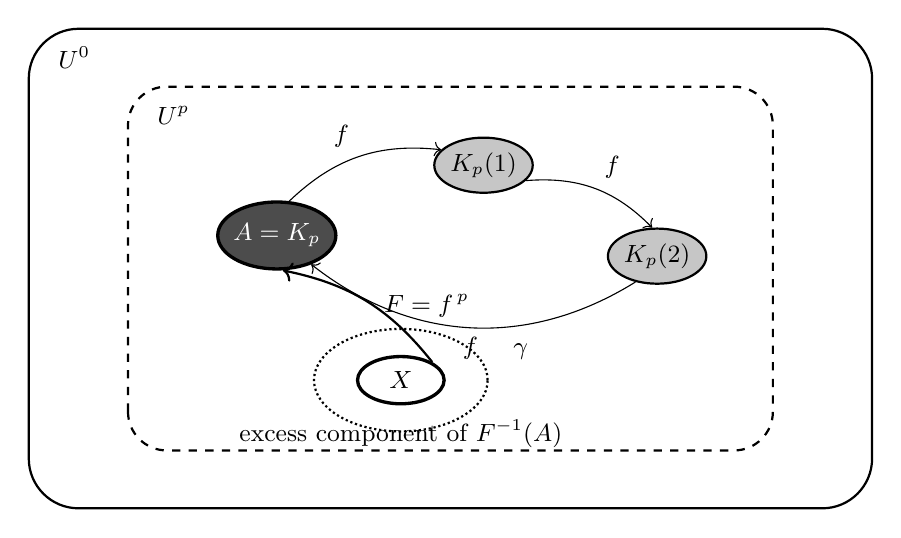
\begin{tikzpicture}[scale=1.05,
  blob/.style={draw, thick, fill=gray!12, rounded corners=6pt},
  julia/.style={draw, thick, fill=gray!45},
  juliaA/.style={draw, very thick, fill=black!70},
  lbl/.style={font=\small}]
  % ambient U^0
  \draw[thick, rounded corners=18pt] (-5.1,-2.9) rectangle (5.1,2.9);
  \node[lbl] at (-4.55,2.55) {\(U^{0}\)};
  % U^p
  \draw[thick, dashed, rounded corners=14pt] (-3.9,-2.2) rectangle (3.9,2.2);
  \node[lbl] at (-3.35,1.85) {\(U^{p}\)};
  % the cycle B = K_p(0) u ... u K_p(p-1), p = 3, with A = K_p = K_p(0)
  \node[juliaA, ellipse, minimum width=1.5cm, minimum height=0.85cm] (A) at (-2.1,0.4) {};
  \node[lbl, white] at (A) {\(A=K_p\)};
  \node[julia, ellipse, minimum width=1.25cm, minimum height=0.7cm] (K1) at (0.4,1.25) {};
  \node[lbl] at (0.4,1.25) {\(K_p(1)\)};
  \node[julia, ellipse, minimum width=1.25cm, minimum height=0.7cm] (K2) at (2.5,0.15) {};
  \node[lbl] at (2.5,0.15) {\(K_p(2)\)};
  % cycle arrows under f
  \draw[->, bend left=25] (A.70) to node[lbl, above left] {\(f\)} (K1.160);
  \draw[->, bend left=25] (K1.-20) to node[lbl, above right] {\(f\)} (K2.100);
  \draw[->, bend left=35] (K2.-130) to node[lbl, below] {\(f\)} (A.-40);
  % excess component X of F^{-1}(A)
  \node[draw, very thick, fill=white, ellipse, minimum width=1.1cm, minimum height=0.6cm]
    (X) at (-0.6,-1.35) {};
  \node[lbl] at (-0.6,-1.35) {\(X\)};
  \node[lbl] at (-0.6,-2.0) {excess component of \(F^{-1}(A)\)};
  \draw[->, bend right=20, thick] (X.30) to node[lbl, right, pos=0.45] {\(F=f^{\,p}\)} (A.-80);
  % the based loop gamma around X
  \draw[thick, densely dotted] (-0.6,-1.35) ellipse (1.05cm and 0.62cm);
  \node[lbl] at (0.85,-1.0) {\(\gamma\)};
\end{tikzpicture}
\caption{The canonical seed of a primitive renormalization of period \(p\)
(drawn for \(p=3\)).  The cycle
\(B=\mathcal K_p=\bigcup_{j}K_p(j)\) is removed and the central continuum
\(A=K_p\) is retained on both sides.  Because \(\deg F=2^{p}\) exceeds the
central degree \(2\), the preimage \(F^{-1}(A)\) has a component
\(X\neq A\).  A based loop \(\gamma\) encircling \(X\) lies outside the
source localization subgroup but is contracted by the physical inclusion in
the target: its localized lift has distinct endpoints that the localized
inclusion identifies.}
\label{fig:seed}
\end{figure}
\begin{figure}[t]
\centering
\begin{tikzcd}[row sep=large, column sep=huge]
  T'_{A}
    \arrow[r, "\widehat{\imath}"]
    \arrow[d, "\pi_{s}"']
  & T_{A}
    \arrow[d, "\pi_{t}"]
  \\
  T' = (U^{p}\setminus F^{-1}B)\cup A
    \arrow[r, hook, "i^{p}"']
  & T = (U^{0}\setminus B)\cup A
\end{tikzcd}
\caption{The localization covers.  The covers \(\pi_{s},\pi_{t}\) are the
based covers classified by the localization subgroups
\(H_{s}\le\pi_{1}(T'\setminus A)\) and \(H_{t}\le\pi_{1}(T\setminus A)\); the localized inclusion
\(\widehat{\imath}\) is the unique based lift of the physical inclusion
\(i^{p}\).  The forced collision is the statement that
\(\widehat{\imath}\) is never injective at an ordinary primitive canonical
seed of period \(p>1\): the class \([\gamma]\) of
Figure~\ref{fig:seed} lies outside \(H_{s}\) while
\((i^{p})_{*}[\gamma]\) is trivial in \(H_{t}\).}
\label{fig:covers}
\end{figure}

This section proves Theorem~\ref{thm:A}.  The mechanism is summarized
by Figures~\ref{fig:seed} and~\ref{fig:covers}: the degree budget
produces an excess component $X$ of $F^{-1}(A)$; peripheral isolation
puts an isolating Jordan disk around $X$; the winding number about $X$
defines a homomorphism killing the source localization subgroup but not
the peripheral class; and the target contracts the peripheral loop
across the isolating disk, since the target removes only $B$ while the
source removes all of $F^{-1}B$.

% New lemmas addressing review items A, B, and the completion step.

\begin{lemma}[Jordan neighborhoods are local pairs]\label{lem:local-pair}
Let $A\subset\mathbb C$ be a nondegenerate full continuum compactly
contained in a Jordan disk $D_A$.  Then $D_A\setminus A$ is a
topological annulus; in particular $(D_A,A)$ is a local pair in the
sense of the localization construction
(Definition~\ref{def:localization}).
\end{lemma}

\begin{proof}
A connected component of $D_A\setminus A$ whose closure does not meet
$\partial D_A$ would be a bounded component of $\mathbb C\setminus A$,
contradicting fullness of $A$; hence $D_A\setminus A$ is connected.
In the sphere $\widehat{\mathbb C}$, the complement of $D_A\setminus A$
has exactly the two components $A$ and
$\widehat{\mathbb C}\setminus D_A$, so $D_A\setminus A$ is a doubly
connected plane domain, i.e.\ an annulus.  Its fundamental group is
infinite cyclic, generated by a core curve, which is the defining
property of a local pair.
\end{proof}

\begin{definition}[Shared local neighborhood and based subgroup
representatives]\label{def:shared-neighborhood}
Fix once and for all a Jordan disk $D_A\supset A$ with
$\overline{D_A}\subset U^{p}$ and
$\overline{D_A}\cap\bigl(F^{-1}B\setminus A\bigr)=\varnothing$; such a
disk exists because $F^{-1}B\setminus A$ is a compact set disjoint from
the component $A$ of $F^{-1}B$.  Since
$\Omega_s=T'\setminus A\subset T\setminus A=\Omega_t$ and
$D_A\setminus A\subset\Omega_s$, the same disk is a valid local
neighborhood on both sides.  With a common basepoint and connecting
path fixed in $D_A\setminus A$, define
\[
 H_s=\operatorname{im}\bigl[\pi_1(D_A\setminus A)\to\pi_1(\Omega_s)\bigr],
 \qquad
 H_t=\operatorname{im}\bigl[\pi_1(D_A\setminus A)\to\pi_1(\Omega_t)\bigr].
\]
These are the based representatives of the localization subgroups used
throughout; the collision certificate is representative-independent
(the winding homomorphism kills every conjugate of $H_s$).
\end{definition}

\begin{lemma}[Injectivity of the completion]\label{lem:completion-injective}
In the connected-complement localization construction
(Theorem~\ref{thm:kahn-localization}), the natural map from the
complement covering surface $\widehat\Omega$ into the completed
localized surface $S_A$ is injective.
\end{lemma}

\begin{proof}
The completed surface is the quotient of the disjoint union
$U\sqcup\widehat\Omega$ in which each point $u\in U\setminus A$ is
identified with its image $\ell(u)\in\widehat\Omega$ under the
canonical lift $\ell$ of $U\setminus A$.  Every identification therefore
pairs one point of $U$ with one point of $\widehat\Omega$; no two
points of $\widehat\Omega$ are ever identified with one another, since
$\ell$ is single-valued.  Hence the composition
$\widehat\Omega\hookrightarrow U\sqcup\widehat\Omega\to S_A$ is
injective.
\end{proof}

\begin{remark}\label{rem:completion-consequence}
Lemma~\ref{lem:completion-injective}, applied on both sides, shows that
the filled completion identifies no pair of distinct complement-cover
points.  Consequently every point collision of the completed localized
inclusion $\widehat\imath$ arises from a collision of the
complement-cover lift $\widehat a$, and conversely; this is the bridge
invoked in Theorem~\ref{thm:forced-collision}, now proved rather than
delegated to the verification checklist of
Section~\ref{sec:verification}.
\end{remark}


% ---- begin C:thm_05 ----
% Concordance: manual equation tags (n.m) in this file mirror the numbering of the underlying research note kl_canonical_localization_forced_collision.md, not this paper's section numbering.
\begin{proposition}[Excess central pullback]\label{prop:excess}
There is a component
\[
 X\subset F^{-1}A,\qquad X\ne A.                    \tag{4.1}
\]
Every such component satisfies
\[
 X\cap B=\varnothing.                                \tag{4.2}
\]
\end{proposition}

\begin{remark}[Complete component certificate]\label{rem:certificate}
By Corollary \ref{cor:finite-pullback} the family of excess components is finite.  Fix any deterministic order on the finite pulled-component inventory and choose the first \(X\); no theorem depends on this choice.  Its complete finite itinerary is
\[
 \tau(X)=\bigl(X,\ f(X),\dots,f^p(X)=A;\ \varsigma_0,\dots,\varsigma_{p-1}\bigr),  \tag{4.4}
\]
where \(\varsigma_r\) records the actual component (sheet) of \(f^{-1}(f^{r+1}X)\) containing \(f^rX\).  If a stage already carries external or puzzle markings, those markings order the \(\varsigma_r\); otherwise (4.4) is a geometric component itinerary, not an invented symbolic word.  By Corollaries \ref{cor:finite-pullback} and \ref{cor:isolating-disks} there is a Jordan domain \(D_X\Subset U^p\) with
\[
 X\subset D_X,\qquad \overline D_X\cap\bigl((F^{-1}B\setminus X)\cup B\bigr)=\varnothing.  \tag{4.5}
\]
The peripheral access used in the collision is the based homotopy class of \(\partial D_X\): a genuine access in the complement of the actual pulled obstacle family, not a ribbon-tree label.
\end{remark}

\begin{proof}
The global map \(F=f^p\colon U^p\to U^0\) is proper of degree \(2^p\) (Kahn~I, \S6, p.~31).  By the definition of the primitive quadratic-like renormalization, the central component \(A\) has local degree two under \(F\) (Kahn~I, \S7.4.3, p.~45).

Choose a sufficiently small Jordan neighborhood \(V\) of \(A\) inside the range of the quadratic-like renormalization.  The central component of \(F^{-1}(V)\) maps onto \(V\) with degree two.  The degrees of all components of \(F^{-1}(V)\) sum to \(2^p\), and since \(p>1\),
\[
 2^p-2>0,
\]
so there is a component \(W\) of \(F^{-1}(V)\) other than the central one.  The proper map \(F\colon W\to V\) is onto, so \(W\) contains a point of \(F^{-1}(A)\).  The component \(X\) of \(F^{-1}(A)\) through that point lies in \(W\), hence is not the central component \(A\).  This proves (4.1).

For \(0\le j<p\) write \(K_j=K_p(j)=f^j(A)\).  Since \(F=f^p\) commutes with \(f^j\) on these sets and \(F(A)=A\),
\[
 F(K_j)=f^j(F(A))=f^j(A)=K_j.                       \tag{4.3}
\]
Suppose \(X\cap K_j\ne\varnothing\).  If \(j\ne0\), a point of the intersection is mapped by \(F\) into both \(A\) (because \(X\subset F^{-1}A\)) and \(K_j\) (by (4.3) and invariance), contradicting the primitive disjointness \(A\cap K_j=\varnothing\).  If \(j=0\), then \(X\cap A\ne\varnothing\), so the two connected subsets \(X\) and \(A\) of \(F^{-1}A\) lie in one component, forcing \(X=A\), again a contradiction.  Hence (4.2).
\end{proof}
% ---- end C:thm_05 ----
% ---- begin C:thm_06 ----
% Concordance: manual equation tags (n.m) in this file mirror the numbering of the underlying research note kl_canonical_localization_forced_collision.md, not this paper's section numbering.
\begin{theorem}[Localization subgroup defect]\label{thm:subgroup-defect}
Let \(X\) and \(D_X\) be as in Proposition \ref{prop:excess} and (4.5), and let \(H_s\), \(H_t\) be the localization subgroups of (5.2).  Let \(\eta\subset\Omega_s\) be any path from \(z_*\) to \(\partial D_X\) and set
\[
 \gamma=\eta*\partial D_X*\eta^{-1}.       \tag{5.3}
\]
Then
\[
 [\gamma]\notin H_s,\qquad a_*[\gamma]=1\in H_t,
\]
and consequently
\[
 a_*^{-1}(H_t)\supsetneq H_s:                          \tag{5.7}
\]
the exact failure of the subgroup-reflection equality on the actual canonical-localization data.
\end{theorem}

\begin{proof}
First, \(a=i^p\) maps \(\Omega_s\) into \(\Omega_t\): if \(z\in B\), then \(z\in K_j\) for some \(j\), so \(F(z)\in F(K_j)=K_j\subset B\) by (4.3); hence \(B\subset F^{-1}B\), and therefore \(U^p\setminus F^{-1}B\subset U^0\setminus B\).

The removed family \(F^{-1}B\) is a finite union of pairwise disjoint full continua by Corollary \ref{cor:finite-pullback}, so \(\Omega_s=U^p\setminus F^{-1}B\) is path connected by Lemma \ref{lem:connectivity}; the path \(\eta\) exists, and \(\gamma\) of (5.3) is a well-defined based loop at \(z_*\).

Fix \(x\in X\).  Winding number about \(x\) defines a homomorphism \(\operatorname{Ind}_x\) on \(\pi_1(\Omega_s,z_*)\), since \(x\in X\subset F^{-1}B\) is disjoint from \(\Omega_s\).  Every element of \(H_s\) is represented, before inclusion, by a loop in \(D_A\setminus A\); the Jordan disk \(D_A\) is disjoint from every component of \(F^{-1}B\) other than \(A\), so \(x\notin D_A\), and any loop inside the simply connected \(D_A\) is null-homotopic in \(\mathbb C\setminus\{x\}\).  Consequently
\[
 \operatorname{Ind}_x(H_s)=\{0\}.                     \tag{5.4}
\]
On the other hand, the path and reverse path in (5.3) cancel in winding number, while \(\partial D_X\) (positively oriented) has winding number one about \(x\in X\subset D_X\).  Thus
\[
 \operatorname{Ind}_x(\gamma)=1,\qquad [\gamma]\notin H_s.  \tag{5.5}
\]
For the target: (4.5) gives \(\overline D_X\cap B=\varnothing\), and \(D_X\subset U^p\subset U^0\); hence \(D_X\subset\Omega_t\), and \(\partial D_X\) contracts across the disk \(D_X\) inside \(\Omega_t\).  Therefore
\[
 a_*[\gamma]=1\in H_t.                                \tag{5.6}
\]
Combining (5.5) and (5.6), \([\gamma]\in a_*^{-1}(H_t)\setminus H_s\), which is (5.7).
\end{proof}
% ---- end C:thm_06 ----
% ---- begin C:thm_07 ----
% Concordance: manual equation tags (n.m) in this file mirror the numbering of the underlying research note kl_canonical_localization_forced_collision.md, not this paper's section numbering.
\begin{theorem}[Forced collision at ordinary primitive canonical seeds]\label{thm:forced-collision}
Let \(f\colon U^1\to U^0\) be an ordinary quadratic-like restriction of a quadratic polynomial, primitively renormalizable of period \(p>1\), and let
\[
 \widehat i\colon T'_A\longrightarrow T_A
\]
be Kahn's localized inclusion of the canonical renormalization (the dynamical localization of \((i^p,F)\) at \(A=K_p\) with removal of \(B=\mathcal K_p\)).  Then \(\widehat i\) is \emph{not injective}.  More precisely, there are a component \(X\ne A\) of \(F^{-1}A\), a based loop \(\gamma\subset U^p\setminus F^{-1}B\), and localization subgroups \(H_s\), \(H_t\) such that
\[
 [\gamma]\notin H_s,\qquad (i^p)_*[\gamma]=1\in H_t,   \tag{1.2}
\]
and the lift of \(\gamma\) to the source localization cover has distinct endpoints which \(\widehat i\) identifies.
\end{theorem}

\begin{remark}[Collision certificate]\label{rem:collision-certificate}
The proof yields the explicit certificate
\[
 \mathfrak C_{\mathrm{can}}=\bigl(X,\ D_X,\ [\gamma],\ \tau(X),\ H_s,\ H_t,\ H_s,\ H_s[\gamma],\ \widehat z_*,\ \widehat z_*',\ \widehat a(\widehat z_*)\bigr),  \tag{6.3}
\]
recording the first excess component, the peripheral access, the complete \(p\)-step component itinerary, the source and target subgroups, the two distinguished source cosets, the distinct source sheets, and the common target point.  No critical-value crossing and no numerical approximation is used to create the collision.
\end{remark}

\begin{proof}
Take \(X\), \(D_X\), \(\gamma\), \(H_s\), \(H_t\) from Proposition \ref{prop:excess}, Remark \ref{rem:certificate}, and Theorem \ref{thm:subgroup-defect}; then (1.2) is (5.5)--(5.6).

Let \(\pi_s\colon\widehat\Omega_s\to\Omega_s\) and \(\pi_t\colon\widehat\Omega_t\to\Omega_t\) be the localization covers, corresponding to the subgroups \(H_s\) and \(H_t\) (Kahn~I, \S7.4.1, Theorem~7.12, p.~44), and let \(\widehat a\colon\widehat\Omega_s\to\widehat\Omega_t\) be the unique commuting lift of \(a=i^p\).  Choose a source lift \(\widehat z_*\in\pi_s^{-1}(z_*)\) and lift \(\gamma\) from \(\widehat z_*\); write \(\widehat z_*'\) for the terminal endpoint of the lifted path.  By the covering-subgroup endpoint criterion --- a loop lifts closed at \(\widehat z_*\) exactly when its class lies in \(H_s\) --- together with (5.5),
\[
 \widehat z_*'\ne\widehat z_*.                        \tag{6.1}
\]
The \(\widehat a\)-image of the lifted path is the target lift, from \(\widehat a(\widehat z_*)\), of the loop \(a\circ\gamma\).  By (5.6) the class of \(a\circ\gamma\) is trivial, in particular lies in \(H_t\), so this target lift is closed.  Therefore
\[
 \widehat a(\widehat z_*')=\widehat a(\widehat z_*).  \tag{6.2}
\]
Both points lie in the complementary annulus part of the localized source.  Completing the localized marked surfaces by adjoining the marked continuum \(A\) glues \(A\) in along a local neighborhood and does not identify distinct points of the complement cover.  Thus (6.1)--(6.2) exhibit two distinct points of \(T'_A\) with equal \(\widehat i\)-image in \(T_A\): an actual point collision of Kahn's localized inclusion.

In path language: if \(\alpha\) is any source path from the marked base access to \(z_*\), the two classes \([\alpha]\) and \([\alpha*\gamma]\) are distinct in the source localization and equal after target localization.  Kahn's forward path-equivalence statement (Kahn~I, \S7.4.5, pp.~46--47) --- source-equivalent paths become target-equivalent --- is respected; it is the (unstated) converse that fails.
\end{proof}

\begin{remark}[Compatibility with the embedded inner collar]
\label{rem:collar-compat}
The published sources state that \(i\) \emph{is} an embedding near the
filled set: Kahn~I, Theorem~7.3, p.~37 produces \(U\supset K\) with
\(U'=f^{-1}U\) such that \(i|_{U'}\) is an embedding and
\(\operatorname{mod}(U\setminus i(U'))\ge\mu>0\); Kahn~I,
Lemma~7.4(2), p.~37 gives the uniformized form (an embedding on a round
sub-annulus adjacent to the inner end); and KL~II, Lemma~3.1, p.~10
repeats that \(i\) is an embedding in a neighborhood of \(K'\).  Read
quickly, this looks like a contradiction of
Theorem~\ref{thm:forced-collision}.  It is not: the two statements
concern disjoint parts of the source, and it is worth locating the
collision precisely.

Theorem~\ref{thm:forced-collision} places the colliding points on the
lift of the peripheral loop \(\gamma\) around the excess component
\(X\).  By Proposition~\ref{prop:excess}, \(X\) is a component of
\(F^{-1}(A)\) with \(X\neq A\) and \(X\cap B=\varnothing\), and its
isolating disk \(D_X\) is disjoint from the isolating disk \(D_A\) of
the central continuum.  Thus \(\gamma\) lies in the \emph{outer} part
of the source \(\Omega_s=U^{p}\setminus F^{-1}B\), at positive
distance from \(A\), whereas Theorem~7.3's embedding statement
concerns a quadratic-like restriction shrunk toward \(K'\): the
collar on which injectivity is proved separates \(K'\) from the outer
end and, being disjoint from \(D_X\), contains no point of
\(|\gamma|\).  Injectivity on an inner collar and noninjectivity on
the complement of that collar are simply different assertions; both
hold.

We emphasize that nothing here weakens the sources.  On the contrary,
the same inner-collar embedding is what supplies the annular degree
\(+1\) in Lemma~\ref{lem:annular-degree}.  What the sources do not
supply, and what the counterexamples of
Appendix~\ref{sec:abstract} exist to forestall, is any extension of
the inner-collar statement to a global one: Theorem~\ref{thm:annulus-nogo}
exhibits a degree-one annular immersion satisfying all the hypotheses
of Kahn's annulus lemma that is nevertheless noninjective, and
Theorem~\ref{thm:psiql-nogo} exhibits a complete abstract
\(\psi\)-quadratic-like pair with a remote self-collision compatible
with the embedded inner collar.  Those examples show that the gap
between ``embedded near \(K'\)'' and ``embedded'' cannot be closed
from the stated hypotheses; the present theorem shows that at the
canonical seed it is not merely open but actually open in the
negative direction.
\end{remark}
% ---- end C:thm_07 ----
% ---- begin C:thm_10 ----
\begin{proposition}[Alignment and realization quantifiers]\label{prop:realization}
Items (1)--(2) below are proved without further hypotheses.
\begin{enumerate}
\item Every first canonical localization of an ordinary primitively \(p\)-renormalizable quadratic polynomial, \(p>1\), has the collision with certificate (6.3).
\item That collision propagates through every pullback depth of that same seed.
\item If, in addition, the same seed carries KL direct-decoration data and is strongly aligned at the relevant depths in the sense of Definition~\ref{def:strong-alignment}, then the corresponding Kahn--Lyubich ambient \(\psi\)-ql arrow, its full tile lifts, and the glued pseudo-piece immersion are noninjective.
\end{enumerate}
Item (3) is an implication about an aligned realized stage.  It does not infer that an arbitrary abstract canonical seed has a particular decoration.
\end{proposition}

\begin{remark}[Separate realization routes; not used here]\label{rem:realization-routes}
A separate realization statement may be supplied either by
\begin{itemize}
\item a named quadratic parameter whose primitive renormalization straightens to a non-satellite KL decoration germ, or
\item the standard primitive-tuning theorem, applied to a primitive postcritically finite quadratic base and a non-satellite quadratic germ.
\end{itemize}
Until such a realization is source-locked, the present results are not used to change an existential statement about a narrower parameter subclass.  What is settled unconditionally is the behavior of the actual canonical-localization map at ordinary primitive canonical seeds: any proof that treats that canonical localization as embedding-preserving is invalid.
\end{remark}

\begin{proof}
Item (1) restates Theorem \ref{thm:forced-collision} together with the certificate of Remark \ref{rem:collision-certificate}.  Item (2) restates Theorem \ref{thm:propagation}(1)--(2), proved in Section~\ref{sec:tiles} below.  Item (3) restates Theorem \ref{thm:propagation}(3)--(4), also proved in Section~\ref{sec:tiles} below; no circularity arises from the forward reference, since nothing before Section~\ref{sec:tiles} uses items (2)--(3).  Its hypotheses --- that the seed carries KL direct-decoration data and is strongly aligned at the relevant depths in the sense of Definition~\ref{def:strong-alignment} --- are carried verbatim into the conclusion and are not discharged here.  No realization claim is made, and no empty-class or stage-alignment inference is hidden in any of the three items.
\end{proof}

\begin{remark}[KL-facing item and strong alignment]
\label{rem:realization-alignment}
Item (3) is the Kahn--Lyubich-facing item: it restates the KL-facing
items (3)--(4) of Theorem~\ref{thm:propagation}, and it carries the
strong stage-alignment hypothesis
(Definition~\ref{def:strong-alignment} of Section~\ref{sec:tiles})
explicitly in its statement.  This is as it must be: existence of the
KL direct-decoration data alone does not supply the identifications
\(\Theta_m,\Theta_n\) required by that definition, which is exactly
why item (3) assumes strong alignment in addition to the decoration
data.
\end{remark}
% ---- end C:thm_10 ----

%=====================================================================
\section{The canonical sheet resolution and the infinite defect}
\label{sec:resolution}

\begin{figure}[t]
\centering
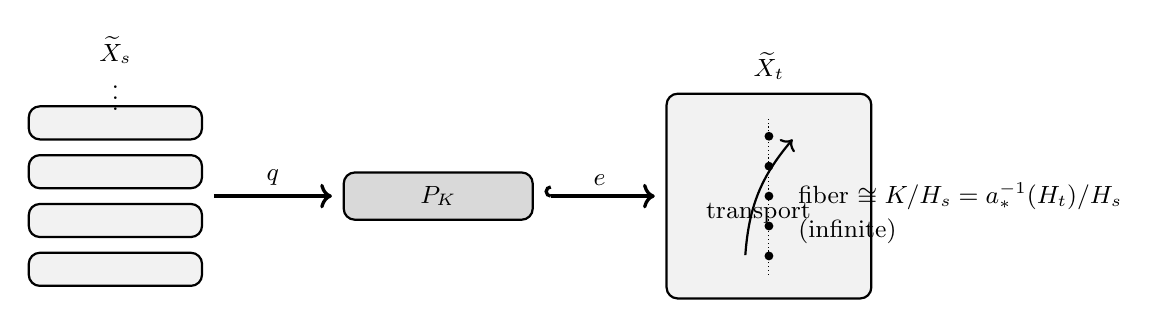
\begin{tikzpicture}[scale=1.0,
  sheet/.style={draw, thick, rounded corners=4pt, fill=gray!10},
  lbl/.style={font=\small}]
  % source resolved cover: stack of sheets
  \foreach \k in {0,1,2,3} {
    \node[sheet, minimum width=2.2cm, minimum height=0.42cm]
      at (-4.1, {0.62*\k - 0.93}) {};
  }
  \node[lbl] at (-4.1, 1.85) {\(\widetilde X_{s}\)};
  \node[lbl] at (-4.1, 1.35) {\(\vdots\)};
  % middle embedded factor P_K
  \node[sheet, fill=gray!30, minimum width=2.4cm, minimum height=0.6cm] (PK) at (0,0) {};
  \node[lbl] at (0, 0) {\(P_{K}\)};
  % target cover
  \node[sheet, minimum width=2.6cm, minimum height=2.6cm] (Xt) at (4.2,0) {};
  \node[lbl] at (4.2, 1.65) {\(\widetilde X_{t}\)};
  % maps
  \draw[->, very thick] (-2.85,0) -- node[lbl, above] {\(q\)} (-1.35,0);
  \draw[{Hooks[right]}->, very thick] (1.35,0) -- node[lbl, above] {\(e\)} (2.75,0);
  % coset fiber column inside X_t
  \foreach \k in {-2,-1,0,1,2} {
    \fill (4.2, {0.38*\k}) circle (1.6pt);
  }
  \draw[densely dotted] (4.2,-1.0) -- (4.2,1.0);
  \node[lbl, right] at (4.45, 0.0) {fiber \(\cong K/H_{s}=a_{*}^{-1}(H_{t})/H_{s}\)};
  \node[lbl, right] at (4.45, -0.45) {(infinite)};
  % transport arrow
  \draw[->, bend left=18, thick] (3.9, -0.75) to node[lbl, below] {transport} (4.5, 0.72);
\end{tikzpicture}
\caption{The canonical intermediate-cover resolution.  The unresolved
immersed pseudo-piece is replaced by the factorization
\(\widetilde X_{s}\xrightarrow{\,q\,}P_{K}\lhook\joinrel\xrightarrow{\,e\,}\widetilde X_{t}\):
a covering onto the embedded intermediate factor (unique in the based
commuting comparison class) followed by an
embedding.  The sheet fiber over the embedded factor is a coset space
detected by the winding homomorphism; it is infinite, and canonical
transport moves sheets along paths in the base.  Exact Kahn base change
preserves the entire structure.}
\label{fig:sheets}
\end{figure}

This section proves Theorems~\ref{thm:B} and~\ref{thm:C}.  The results
are stated for an abstract based embedding $a$ between bases of
connected covers, with based lift $A$.  The factorization is summarized
by Figure~\ref{fig:sheets}.

\emph{Notational scope:} within
Sections~\ref{sec:resolution}--\ref{sec:wholetile} several symbols are
reused in the abstract covering and tile settings, and each is to be
resolved at its local declaration.  Specifically: $A$ is the localized
lift of the base embedding $a$ (here and again in
Section~\ref{sec:basechange}), not the marked continuum $A=K_{p}$ of
Sections~\ref{sec:background}--\ref{sec:forced}; $K=a_{*}^{-1}(H_{t})$
is the reflected subgroup, not a filled Julia set; $T$ names the target
of the resolved factorization in
Definition~\ref{def:canonical-resolved-system}, not the marked surface
$(U^{0}\setminus B)\cup A$; $H=\langle h\rangle$ is the wrapping group
of the annular-tower typing in Section~\ref{sec:wholetile}, distinct
from the localization subgroups $H_{s},H_{t}$; $q$ and $e$ denote the
resolved covering and embedding legs (with tower iterates
$q_{r},e_{r}$), while in the direct-decoration depth formulas
$m=\nu q+1$, $n=(\nu-1)q+1$ of Section~\ref{sec:tiles} the letter $q$
is the Kahn--Lyubich decoration period; $L$ denotes the intermediate
subgroup in the proof of Theorem~\ref{thm:unique-intermediate} and, in
Sections~\ref{sec:tiles}--\ref{sec:wholetile}, a universal-cover tile
lift; $P$ denotes the pullback $X_{s}\times_{X_{t}}\widehat X_{t}$
(with basepoint component $P_{K}$) in this section and the
Kahn--Lyubich decoration piece $P=Y^{(\nu-1)q+1}$ in
Section~\ref{sec:tiles}; and $\mathbf U^{r}$ denotes the
complementary-cover equalizer stage of Sections~\ref{sec:forced}
and~\ref{sec:basechange}, whose two usages are reconciled by the
identity $i_{r}^{-1}(K^{r})=K^{r+1}=f_{r}^{-1}(K^{r})$: the
complement-locus equalizer is the complement of the equalizer's filled
set, so the stagewise complementary annuli
$A_{r}=\mathbf U^{r}\setminus K^{r}$ are well defined at every depth.

The canonical
localization of Section~\ref{sec:forced} is the instantiation
$a=i^{p}$, $X_{s}=\Omega_{s}$, $X_{t}=\Omega_{t}$, $A=\widehat a$ (the
complement-cover lift of Theorem~\ref{thm:forced-collision}); Kahn's
localized inclusion $\widehat\imath$ is obtained from $\widehat a$ by
the filled completion, which identifies no complement-cover points.
The pointed
coset set $K/H_{s}$ is \emph{not} asserted to be a group unless
$H_{s}\trianglelefteq K$ is separately proved.

% ---- begin D:notation ----
%% ---------- Notation and standing conventions for Cluster D ----------
%% Source: kl_localization_sheet_resolution_factorization.md, Sec. 2-3 (lines 62-183)
\subsection*{Notation and standing conventions}

All spaces in this part are Hausdorff, connected, locally path-connected,
and semilocally simply connected; all covering spaces are connected and
based.  These hypotheses are satisfied by the planar complementary
surfaces used in the canonical KL localization.  Path products and
induced fundamental-group maps are based; every statement involving an
unbased cover or subgroup is to be read after the displayed basepoints
have been fixed.

For a based covering \( p\colon(\widehat X,\widehat x)\to(X,x) \) we write
\[
  H \;=\; p_*\pi_1(\widehat X,\widehat x)\;\leq\;\pi_1(X,x)
\]
for its characteristic subgroup.

For subgroups \( H\leq K \) of a group,
\begin{equation}\label{eq:coset-set}
  K/H=\{\,kH : k\in K\,\}
\end{equation}
denotes only the \emph{pointed set} of cosets with distinguished point
\( H \).  No multiplication on \eqref{eq:coset-set} is asserted unless
\( H\triangleleft K \).  With the usual path-endpoint convention a cover
fiber is naturally the right-coset set \( H\backslash K \); inversion
gives the canonical pointed bijection \( Hk\longmapsto k^{-1}H \) with
\eqref{eq:coset-set}.  Thus the notation \( K/H \) does not silently
assume normality.

For composable paths we use the paper-wide convention of
Section~\ref{sec:background}: \( \delta_1*\delta_2 \) means first
traverse \( \delta_1 \), then traverse \( \delta_2 \), and in
fundamental groups \( [\delta_1][\delta_2]=[\delta_1*\delta_2] \)
(the first-traversed factor is written leftmost).  In the endpoint
description, continuing the fiber point labelled \( H_sk \) by a based
loop \( g \) appends \( g \) after \( k \) and gives \( H_skg \); under
the inversion identification
\( H_sk\mapsto k^{-1}H_s \), that transport is
\begin{equation}\label{eq:transport-formula}
  k^{-1}H_s\;\longmapsto\; g^{-1}k^{-1}H_s .
\end{equation}
Formula \eqref{eq:transport-formula} replaces any naive multiplication on
\( K/H_s \) and remains valid when \( H_s \) is not normal in \( K \).

Fixed symbols of this part:
\( a\colon(X_s,x_s)\hookrightarrow(X_t,x_t) \) is a based topological
embedding (at the canonical KL primitive seed the spaces are the
complementary surfaces, \( X_s=\Omega_s \), \( X_t=\Omega_t \), and
\( a=i^{p} \));
\( p_s\colon(\widehat X_s,\widehat x_s)\to(X_s,x_s) \) and
\( p_t\colon(\widehat X_t,\widehat x_t)\to(X_t,x_t) \) are connected based
covers with subgroups \( H_s,H_t \);
\( A\colon(\widehat X_s,\widehat x_s)\to(\widehat X_t,\widehat x_t) \) is a
based lift satisfying \( p_tA=ap_s \);
\( K:=a_*^{-1}(H_t)\leq\pi_1(X_s,x_s) \);
\( P=X_s\times_{X_t}\widehat X_t \) is the pullback and \( P_K \) the path
component of the basepoint \( (x_s,\widehat x_t) \), with first and second
projections \( r \) and \( e \);
\( q\colon\widehat X_s\to P_K \) is the canonical comparison map of
Theorem~\ref{thm:sheet-resolution};
\( \mathcal S_{\mathrm{loc}}=K/H_s \) is the based localization-sheet
fiber;
\( M_\delta \) denotes sheet transport along a path \( \delta \) in
\( P_K \); \( \Pi_1(P_K) \) is the fundamental groupoid of \( P_K \); and
\( \mathcal G_q \) is the canonical sheet-transport groupoid of
Proposition~\ref{prop:transport}.  \( \mathbf{Set}_{\mathrm{bij}} \)
denotes the category of sets and bijections.  A map defined on an open
interval is \emph{topologically proper} if preimages of compact sets are
compact.

%% Typographic note: the source note writes \mathcal{S}_{loc} and
%% \mathcal{G}_q; we use \mathcal{S}_{\mathrm{loc}} and \mathcal{G}_q to
%% remain within amssymb (no mathrsfs).  The source's amscd square in
%% Corollary 7.2 is rendered as a displayed commutation equation.
% ---- end D:notation ----
% ---- begin D:definitions ----
\begin{definition}[Canonical localization covering data]\label{def:loc-data}
Let \( a\colon(X_s,x_s)\hookrightarrow(X_t,x_t) \) be a based topological
embedding, and let
\( p_s\colon(\widehat X_s,\widehat x_s)\to(X_s,x_s) \),
\( p_t\colon(\widehat X_t,\widehat x_t)\to(X_t,x_t) \)
be connected based covers with characteristic subgroups \( H_s \),
\( H_t \).  Suppose a based lift
\( A\colon(\widehat X_s,\widehat x_s)\to(\widehat X_t,\widehat x_t) \)
exists with
\begin{equation}\label{eq:lift-square}
  p_t A = a p_s .
\end{equation}
The lifting criterion then gives \( a_*(H_s)\leq H_t \).  Define
\begin{equation}\label{eq:K-def}
  K := a_*^{-1}(H_t)\;\leq\;\pi_1(X_s,x_s),
\end{equation}
so that \( H_s\leq K \).
\end{definition}

\begin{definition}[Canonical pullback component]\label{def:pullback-component}
With the data of Definition~\ref{def:loc-data}, form the pullback
\begin{equation}\label{eq:pullback}
  P = X_s\times_{X_t}\widehat X_t
    = \bigl\{(x,\widehat y): a(x)=p_t(\widehat y)\bigr\},
\end{equation}
and let \( P_K \) be the path component of the basepoint
\( (x_s,\widehat x_t) \).  Write
\begin{equation}\label{eq:legs}
  r\colon P_K\to X_s,\quad r(x,\widehat y)=x,
  \qquad
  e\colon P_K\to\widehat X_t,\quad e(x,\widehat y)=\widehat y .
\end{equation}
\end{definition}

\begin{definition}[Sheet transport]\label{def:sheet-transport}
Let \( q\colon\widehat X_s\to P_K \) be the covering of
Theorem~\ref{thm:sheet-resolution}.  For every path
\( \delta\colon[0,1]\to P_K \) and every
\( \widehat u\in q^{-1}(\delta(0)) \), let
\( \widetilde\delta_{\widehat u} \) be the unique \( q \)-lift of
\( \delta \) beginning at \( \widehat u \), and define
\begin{equation}\label{eq:transport-def}
  M_\delta(\widehat u)
  = \widetilde\delta_{\widehat u}(1)
  \in q^{-1}(\delta(1)).
\end{equation}
\end{definition}

\begin{definition}[Enlargement data and the based coset map]\label{def:coset-map}
Let
\( H\leq K\leq G \) and \( H^+\leq K^+\leq G^+ \) be subgroup chains, and
let \( \varphi\colon G\to G^+ \) be a homomorphism such that
\begin{equation}\label{eq:coset-map-hyp}
  \varphi(H)\leq H^+,
  \qquad
  \varphi(K)\leq K^+ .
\end{equation}
Then
\begin{equation}\label{eq:coset-map-def}
  \overline\varphi\colon K/H\longrightarrow K^+/H^+,
  \qquad
  kH\longmapsto \varphi(k)H^+
\end{equation}
is well defined: if \( k_1H=k_2H \) then \( k_2^{-1}k_1\in H \), so
\( \varphi(k_2)^{-1}\varphi(k_1)\in\varphi(H)\leq H^+ \), whence
\( \varphi(k_1)H^+=\varphi(k_2)H^+ \).
\end{definition}
% ---- end D:definitions ----
% ---- begin D:thm_00 ----
\begin{lemma}[Subgroup of the pullback component]\label{lem:pullback-subgroup}
With the data of Definitions~\ref{def:loc-data} and~\ref{def:pullback-component}, the first projection \( r\colon P_K\to X_s \) is the connected based cover of \( X_s \) corresponding to the subgroup \( K=a_*^{-1}(H_t) \).
\end{lemma}

\begin{proof}
The pullback of a covering is a covering.  The pullback \( P \) is locally path-connected, so its path components are open.  Moreover, the selected component \( P_K \) maps onto \( X_s \): since a connected, locally path-connected space is path connected, for any \( x\in X_s \) choose a path from \( x_s \) to \( x \); its lift to the pullback from \( (x_s,\widehat x_t) \) stays in \( P_K \) and ends over \( x \).  Hence the restriction \( r\colon P_K\to X_s \) is itself a connected covering.

It remains to compute its subgroup.  Let \( \gamma \) be a based loop in \( X_s \).  Its lift to \( P_K \) from \( (x_s,\widehat x_t) \) is
\begin{equation}\label{eq:pullback-lift}
  t\longmapsto\bigl(\gamma(t),\widehat{a\gamma}(t)\bigr),
\end{equation}
where \( \widehat{a\gamma} \) is the lift of \( a\gamma \) to \( \widehat X_t \) from \( \widehat x_t \).  The lift \eqref{eq:pullback-lift} is closed if and only if \( \widehat{a\gamma} \) is closed.  By the cover--subgroup criterion, this is equivalent to \( a_*[\gamma]\in H_t \), which, by \eqref{eq:K-def}, is equivalent to \( [\gamma]\in K \).  Therefore
\[
  r_*\pi_1\bigl(P_K,(x_s,\widehat x_t)\bigr)=K .
\]
This also proves that the selected path component is precisely the based connected cover classified by \( K \).
\end{proof}
% ---- end D:thm_00 ----
% ---- begin D:thm_01 ----
\begin{lemma}[The resolved leg is embedded]\label{lem:embedded-leg}
The second projection
\begin{equation}\label{eq:e-embedding}
  e\colon P_K\hookrightarrow\widehat X_t
\end{equation}
is a topological embedding.
\end{lemma}

\begin{proof}
First consider the second projection on the entire pullback \( P \).  Its image is \( p_t^{-1}(a(X_s)) \).  Because \( a \) is an embedding, the formula
\begin{equation}\label{eq:e-inverse}
  \widehat y\longmapsto\bigl(a^{-1}(p_t(\widehat y)),\,\widehat y\bigr)
\end{equation}
is a continuous inverse on this image.  Thus the second projection identifies \( P \) homeomorphically with \( p_t^{-1}(a(X_s)) \).  Restricting this homeomorphism to \( P_K \) proves \eqref{eq:e-embedding}.
\end{proof}

\begin{remark}
The embedding hypothesis on \( a \) is essential: if \( a \) has a
base-space self-intersection, equality of second coordinates in
\eqref{eq:pullback} need not determine the first coordinate, and
Lemma~\ref{lem:embedded-leg} can fail before any subgroup collision is
considered; compare Section~\ref{sec:seedvsbold}.
\end{remark}
% ---- end D:thm_01 ----
% ---- begin D:thm_02 ----
\begin{theorem}[Canonical sheet resolution]\label{thm:sheet-resolution}
With the data of Definitions~\ref{def:loc-data} and~\ref{def:pullback-component}, define
\begin{equation}\label{eq:q-def}
  q\colon\widehat X_s\longrightarrow P_K,
  \qquad
  q(\widehat u)=\bigl(p_s(\widehat u),\,A(\widehat u)\bigr).
\end{equation}
Then:
\begin{enumerate}
\item \( q \) is the unique based map over \( X_s \) from the \( H_s \)-cover to the \( K \)-cover;
\item \( q \) is a surjective covering map;
\item the original lift factors exactly as
\begin{equation}\label{eq:factorization}
  A=e\circ q;
\end{equation}
\item for all \( \widehat u,\widehat v\in\widehat X_s \),
\begin{equation}\label{eq:kernel-equiv}
  A(\widehat u)=A(\widehat v)
  \quad\Longleftrightarrow\quad
  q(\widehat u)=q(\widehat v);
\end{equation}
\item equivalently, the kernel pairs agree:
\begin{equation}\label{eq:kernel-pair}
  \widehat X_s\times_{P_K}\widehat X_s
  =
  \widehat X_s\times_{\widehat X_t}\widehat X_s;
\end{equation}
\item the fiber of \( q \) over the based point is the pointed coset set
\begin{equation}\label{eq:sheet-fiber}
  \mathcal S_{\mathrm{loc}}=K/H_s;
\end{equation}
\item \( q \) is injective if and only if \( K=H_s \); and
\item if \( [K:H_s]<\infty \), then \( q \) has exactly \( [K:H_s] \) sheets.  No finiteness is asserted when the index is infinite.
\end{enumerate}
\end{theorem}

\begin{proof}
The formula \eqref{eq:q-def} lands in the pullback \eqref{eq:pullback} because \eqref{eq:lift-square} gives
\[
  a(p_s(\widehat u))=p_t(A(\widehat u)).
\]
It lands in \( P_K \) because \( \widehat X_s \) is path connected and \( q \) sends the basepoint to \( (x_s,\widehat x_t) \).  Moreover,
\begin{equation}\label{eq:rq}
  r q = p_s .
\end{equation}

Since \( H_s\leq K \), the lifting criterion for covers over the common base \( X_s \) gives a unique based map from the \( H_s \)-cover to the \( K \)-cover.  Thus \eqref{eq:q-def} is that map, proving (1).

We verify surjectivity directly rather than hiding it in cover classification.  Let \( z\in P_K \), and choose a path \( \delta \) in \( P_K \) from the based point to \( z \).  Lift \( r\delta \) to \( \widehat X_s \) from \( \widehat x_s \), obtaining a path \( \widehat\delta \).  Both \( \delta \) and \( q\widehat\delta \) are lifts of \( r\delta \) to \( P_K \) from the same initial point.  Uniqueness of path lifting gives
\[
  q(\widehat\delta(1))=\delta(1)=z .
\]
Hence \( q \) is onto.  Choose a path-connected neighborhood \( U\subset X_s \) evenly covered by both \( p_s \) and \( r \).  Each component of \( p_s^{-1}(U) \) is mapped by \( q \) into one component of \( r^{-1}(U) \); because both projections to \( U \) are homeomorphisms and \( rq=p_s \), this restriction of \( q \) is a homeomorphism onto that target sheet.  Surjectivity of \( q \) ensures that every target sheet is met.  Therefore \( q \) is a covering map, proving (2).

The second coordinate in \eqref{eq:q-def} is \( A(\widehat u) \), so \eqref{eq:factorization} is immediate, proving (3).  Since \( e \) is injective by Lemma~\ref{lem:embedded-leg},
\[
  A(\widehat u)=A(\widehat v)
  \iff
  e(q(\widehat u))=e(q(\widehat v))
  \iff
  q(\widehat u)=q(\widehat v),
\]
which proves (4) and (5).

The standard fiber classification for the map from an \( H_s \)-cover to a \( K \)-cover identifies its based fiber with the right-coset set \( H_s\backslash K \).  The inversion convention (\( H_sk\mapsto k^{-1}H_s \)) identifies that pointed set with \( K/H_s \), proving (6).  The map is one-sheeted exactly when the two subgroups agree, proving (7); in finite index its sheet number is \( [K:H_s] \), proving (8).
\end{proof}
% ---- end D:thm_02 ----
% ---- begin D:thm_03 ----
\begin{corollary}[Exact meaning of the forced KL collision]\label{cor:forced-collision-meaning}
For an ordinary primitive KL canonical localization,
Theorem~\ref{thm:forced-collision} (via display (5.7) of
Theorem~\ref{thm:subgroup-defect}) gives
\begin{equation}\label{eq:proper-inclusion}
  H_s\subsetneq K=(i^{p})_*^{-1}(H_t).
\end{equation}
Consequently \( q \) in \eqref{eq:q-def} is a nontrivial covering and \( e \) is an embedded resolved pullback component.  The peripheral loop around the proved excess component gives a non-base point of the based fiber \eqref{eq:sheet-fiber}.  All point collisions of the full localized inclusion \( A \) occur in fibers of this same \( q \); none is left unexplained by the factorization.
\end{corollary}

\begin{proof}
%% The source (lines 363-380) states this corollary with its derivation inline;
%% the following assembles exactly those inline steps.
The proper inclusion \eqref{eq:proper-inclusion} is display (5.7) of Theorem~\ref{thm:subgroup-defect}, supplied at the ordinary primitive canonical seed by Theorem~\ref{thm:forced-collision}.  By Theorem~\ref{thm:sheet-resolution}(7), \( q \) is injective if and only if \( K=H_s \); hence \eqref{eq:proper-inclusion} makes \( q \) a nontrivial (noninjective) covering, while Lemma~\ref{lem:embedded-leg} exhibits \( e \) as a topological embedding of the resolved pullback component.  The peripheral class \( [\gamma] \) supplied by Theorem~\ref{thm:forced-collision} lies in \( K\setminus H_s \), so its coset \( [\gamma]H_s\in K/H_s \) is a non-base point of the based fiber \eqref{eq:sheet-fiber}.  Finally, Theorem~\ref{thm:sheet-resolution}(4)--(5) identify the kernel pair of \( A \) with the kernel pair of \( q \), so every point collision of \( A \) occurs inside a single \( q \)-fiber.
\end{proof}

\begin{remark}
This corollary is unconditional at the canonical primitive seed.  Its
transport to a named KL direct-decoration depth carries the same-seed
alignment qualification of Proposition~\ref{prop:realization}.
\end{remark}
% ---- end D:thm_03 ----
% ---- begin D:thm_04 ----
\begin{corollary}[The canonical sheet defect is infinite]\label{cor:infinite-defect}
At every ordinary primitive canonical seed,
\begin{equation}\label{eq:infinite-index}
  [K:H_s]=\infty .
\end{equation}
Consequently \( q \) is an infinite-sheeted cover, and for every \( z\in P_K \),
\[
  A^{-1}(e(z))=q^{-1}(z)
\]
is infinite.  Equivalently: every non-singleton fiber of the completed localized inclusion (that is, every fiber over the embedded resolved complement component \( e(P_K) \)) is infinite; fibers over the filled part are singletons and are not at issue.  In particular, no finite enumeration of the raw localization sheets can be complete.
\end{corollary}

\begin{proof}
Use the excess component \( X^{\mathrm{exc}} \) (the component denoted \( X \) in Theorem~\ref{thm:forced-collision}, written \( X^{\mathrm{exc}} \) here to avoid the abstract symbols \( X_s,X_t \) of this section), the point \( x\in X^{\mathrm{exc}} \), and the peripheral class \( [\gamma] \) supplied by Theorem~\ref{thm:forced-collision}.  Winding about \( x \) defines a homomorphism
\[
  w\colon\pi_1(\Omega_s,x_s)\longrightarrow\mathbb Z
\]
(here \( x_s=z_* \), the localization basepoint, under the instantiation of this section's scope note).
Every source-local loop is supported in the chosen neighborhood of the central component, which misses \( x \); hence
\[
  w(H_s)=0 .
\]
The peripheral class satisfies
\[
  w([\gamma])=1,
  \qquad
  [\gamma]\in K .
\]
Because \( K \) is a subgroup, \( [\gamma]^n\in K \) for every \( n\in\mathbb Z \).  If two cosets were equal,
\[
  [\gamma]^mH_s=[\gamma]^nH_s,
\]
then \( [\gamma]^{m-n}\in H_s \).  Applying \( w \) would give \( m-n=0 \).  Thus the cosets \( [\gamma]^nH_s \), \( n\in\mathbb Z \), are pairwise distinct, proving \eqref{eq:infinite-index}.

Theorem~\ref{thm:sheet-resolution} identifies the fiber cardinality of \( q \) with this index and identifies the \( A \)-fibers with the \( q \)-fibers, which gives the remaining assertions.
\end{proof}

% Concordance: the manual tag (9.1) below mirrors the numbering of the underlying
% research note kl_canonical_localization_forced_collision.md.
\begin{remark}\label{rem:coset-set}
Here \(K/H_s=a_*^{-1}(H_t)/H_s\) is a pointed set of left cosets; it is not asserted to be a quotient group unless normality of \(H_s\) is separately proved.  Any carrier (e.g.\ a ribbon tree) that identifies these cosets to a point hides the analytic obstruction and is not proof-faithful.  The minimal replacement state recorded by the underlying research notes is
\[
 \mathfrak S_{\mathrm{loc}}=\bigl(\operatorname{Comp}(F^{-1}B),\ \{\tau(X)\},\ H_s,H_t,\ H_s\backslash\pi_1(\Omega_s),\ a_*^{-1}(H_t)/H_s\bigr).  \tag{9.1}
\]
\end{remark}
% ---- end D:thm_04 ----
% ---- begin D:thm_05 ----
\begin{theorem}[Unique embedded intermediate factor]\label{thm:unique-intermediate}
Suppose \( r_C\colon C\to X_s \) is a connected based intermediate cover and
\begin{equation}\label{eq:candidate-factorization}
  \widehat X_s\xrightarrow{\;q_C\;}C\xrightarrow{\;e_C\;}\widehat X_t
\end{equation}
satisfies, with \( q_C \) and \( e_C \) based,
\begin{equation}\label{eq:candidate-compat}
  r_Cq_C=p_s,\qquad p_te_C=ar_C,\qquad A=e_Cq_C,
\end{equation}
and \( e_C \) is injective.  Then the subgroup of \( C\to X_s \) is exactly \( K \), and there is a unique based isomorphism of covers
\begin{equation}\label{eq:unique-iso}
  C\cong P_K
\end{equation}
which identifies \eqref{eq:candidate-factorization} with the canonical factorization \( \widehat X_s\xrightarrow{q}P_K\xrightarrow{e}\widehat X_t \).
\end{theorem}

\begin{proof}
Let
\[
  L=(r_C)_*\pi_1(C)\leq\pi_1(X_s).
\]
Existence of \( q_C \) gives \( H_s\leq L \).  Existence of \( e_C \) gives
\[
  a_*(L)\leq H_t,
\]
so \( L\leq K \).

Apply the subgroup-reflection criterion (Theorem~\ref{thm:subgroup-reflection-criterion}, applied to the covers with subgroups \( L \) and \( H_t \)) to the lift \( e_C\colon C\to\widehat X_t \) of the physical embedding \( a \).  Since \( e_C \) is injective, that criterion gives
\[
  a_*^{-1}(H_t)=L .
\]
The left side is \( K \), hence \( L=K \).  The classification of connected based covers now gives the unique based isomorphism \eqref{eq:unique-iso}, and uniqueness of based lifts identifies both factor maps.
\end{proof}

\begin{remark}
Thus \( P_K \) is the unique connected intermediate cover on which the
remaining leg is embedded; replacing \( K/H_s \) by a coarser finite
label set without proving the corresponding factor injective would
destroy this optimality.
\end{remark}
% ---- end D:thm_05 ----

\subsection{The sheet-transport groupoid}
% ---- begin D:thm_06 ----
\begin{proposition}[Exact sheet transport]\label{prop:transport}
The transport maps \( M_\delta \) of Definition~\ref{def:sheet-transport} satisfy:
\begin{enumerate}
\item \( M_\delta \) is a bijection, with inverse \( M_{\delta^{-1}} \);
\item \( M_\delta \) depends only on the homotopy class of \( \delta \) relative to its endpoints;
\item for composable paths,
\begin{equation}\label{eq:transport-functorial}
  M_{\delta_1*\delta_2}=M_{\delta_2}\circ M_{\delta_1};
\end{equation}
\item the constant path induces the identity; and
\item at the based point these transports give the monodromy action on the pointed fiber \( K/H_s \).
\end{enumerate}
Hence
\begin{equation}\label{eq:transport-functor}
  \Pi_1(P_K)\longrightarrow\mathbf{Set}_{\mathrm{bij}},
  \qquad
  z\longmapsto q^{-1}(z),\quad
  [\delta]\longmapsto M_\delta
\end{equation}
is a functor.  Its category of elements is the canonical sheet-transport groupoid \( \mathcal G_q \).  Its full object set is
\[
  \bigl\{(z,\widehat u): z\in P_K,\ \widehat u\in q^{-1}(z)\bigr\},
\]
canonically the point set of \( \widehat X_s \).  The pointed coset set \( K/H_s \) is only its based fiber (equivalently, the object set after restricting \eqref{eq:transport-functor} to the based action groupoid).
\end{proposition}

\begin{proof}
Every assertion is forced by uniqueness and homotopy invariance of lifts.  Lifting \( \delta \) and then \( \delta^{-1} \) returns to the initial point, which proves bijectivity, giving (1).  A homotopy relative endpoints lifts after an initial sheet is fixed, so the terminal sheet is constant through the homotopy, giving (2).  The lift of a concatenation is the concatenation of the two successive lifts; the first-traversed factor \( \delta_1 \) acts first and therefore appears innermost in the function composition, proving \eqref{eq:transport-functorial} and (3).  Constant paths lift to constant paths, giving (4).  Restricting \eqref{eq:transport-functor} to the based fundamental group gives the usual monodromy action on the cover fiber, identified with \( K/H_s \) by the inversion convention, giving (5).
\end{proof}

\begin{remark}\label{rem:no-regularity}
No regularity of the cover is used.  If \( H_s \) is not normal in \( K \), the based fiber \( K/H_s \) is not a quotient group, but the groupoid \eqref{eq:transport-functor} still gives complete path transport.  Under the inversion convention, continuation by a based loop \( g \) acts by the explicit formula \eqref{eq:transport-formula}, \( k^{-1}H_s\mapsto g^{-1}k^{-1}H_s \), not by a silently assumed quotient-group multiplication.
\end{remark}
% ---- end D:thm_06 ----
% ---- begin D:thm_07 ----
\begin{proposition}[Compact-segment lifting classification]\label{prop:compact-lift}
Let \( \gamma\colon[0,1]\to\widehat X_t \) have image in the embedded resolved component \( e(P_K) \), and put \( \delta=e^{-1}\gamma \).  Then the source paths
\begin{equation}\label{eq:A-lift}
  \widehat\delta\colon[0,1]\to\widehat X_s
  \quad\text{such that}\quad
  A\widehat\delta=\gamma
\end{equation}
are exactly the \( q \)-lifts of \( \delta \).  There is one and only one such path for each initial sheet in \( q^{-1}(\delta(0)) \), and its final sheet is given by \( M_\delta \).

The same statement applies separately on every compact parameter interval on which a target path lies in \( e(P_K) \).
\end{proposition}

\begin{proof}
If \( q\widehat\delta=\delta \), then
\[
  A\widehat\delta=eq\widehat\delta=e\delta=\gamma .
\]
Conversely, if \eqref{eq:A-lift} holds, then
\[
  e(q\widehat\delta)=A\widehat\delta=\gamma=e\delta .
\]
Injectivity of \( e \) (Lemma~\ref{lem:embedded-leg}) gives \( q\widehat\delta=\delta \).  Covering path lifting supplies exactly one lift from each initial sheet, and Proposition~\ref{prop:transport} computes its endpoint.
\end{proof}

\begin{remark}
Proposition~\ref{prop:compact-lift} is the precise compact-segment
replacement for treating \( A \) as an embedding.  It does not
classify a target path which leaves and re-enters \( e(P_K) \), glue
choices over nested intervals, prove convergence to declared prime
ends, or prove the KKL unique-proper-lift predicate.
\end{remark}
% ---- end D:thm_07 ----
% ---- begin D:thm_08 ----
\begin{proposition}[Topological properness, with its exact boundary]\label{prop:properness}
Let \( \delta\colon(0,1)\to P_K \) be topologically proper.  Then every \( q \)-lift \( \widehat\delta\colon(0,1)\to\widehat X_s \) is topologically proper.

If, in addition, \( a(X_s) \) is open in \( X_t \), then \( e(P_K) \) is open in \( \widehat X_t \).  Let \( \gamma\colon(0,1)\to\widehat X_t \) be topologically proper and let \( J \) be a component of \( \gamma^{-1}(e(P_K)) \).  After parametrizing \( J \) as an open interval,
\[
  \delta_J=e^{-1}\gamma|_J
\]
is topologically proper, and so are all of its \( q \)-lifts.
\end{proposition}

\begin{proof}
For compact \( C\subset\widehat X_s \), the set \( q(C) \) is compact.  Therefore
\[
  \widehat\delta^{-1}(C)\subset\delta^{-1}(q(C)).
\]
The right side is compact in \( (0,1) \) by properness of \( \delta \).  Since \( \widehat X_s \) is Hausdorff, \( C \) is closed, so \( \widehat\delta^{-1}(C) \) is closed in \( (0,1) \), hence closed in the right side.  It is therefore compact.  This proves properness of the lift.

If \( a(X_s) \) is open, then \( p_t^{-1}(a(X_s)) \) is open.  Lemma~\ref{lem:embedded-leg} identifies the selected component \( e(P_K) \) with an open component of that preimage.  For compact \( C\subset P_K \),
\[
  \delta_J^{-1}(C)=J\cap\gamma^{-1}(e(C)).
\]
The set
\[
  S=\gamma^{-1}(e(C))
\]
is compact because \( e(C) \) is compact and \( \gamma \) is proper.  Moreover \( S\subset\gamma^{-1}(e(P_K)) \).  The latter set is open in \( (0,1) \), and its components are open intervals which are also closed relative to that open set.  Hence \( J\cap S \) is closed in \( S \), and is compact.  The definition \( \delta_J=e^{-1}\gamma|_J \) identifies \( J\cap S \) with \( \delta_J^{-1}(C) \).  Thus \( \delta_J \) is proper.  Apply the first paragraph to every \( q \)-lift.
\end{proof}

\begin{remark}
Topological properness means escape from compact subsets.  It does not
give convergence to a declared prime end, subordination to one marked
ideal interval, or uniqueness among the infinitely many possible
proper sheet lifts.
\end{remark}
% ---- end D:thm_08 ----

%=====================================================================
\section{Exact enlargement tests}
\label{sec:enlargement}

Root or marking enlargement changes the spaces and the subgroups.  The
following exact tests decide when the old sheet data survives; the
accompanying warnings record why the algebraic tests cannot replace a
geometric audit.

% ---- begin D:thm_09 ----
\begin{theorem}[Based-coset no-merger/no-birth criterion]\label{thm:coset-criterion}
For the based coset map \( \overline\varphi\colon K/H\to K^+/H^+ \) of Definition~\ref{def:coset-map}:
\begin{equation}\label{eq:injectivity-criterion}
  \overline\varphi\ \text{is injective}
  \iff
  K\cap\varphi^{-1}(H^+)=H;
\end{equation}
\begin{equation}\label{eq:surjectivity-criterion}
  \overline\varphi\ \text{is surjective}
  \iff
  K^+=\varphi(K)H^+;
\end{equation}
and therefore
\begin{equation}\label{eq:bijectivity-criterion}
  \overline\varphi\ \text{is bijective}
  \iff
  \begin{cases}
    K\cap\varphi^{-1}(H^+)=H,\\[2pt]
    K^+=\varphi(K)H^+ .
  \end{cases}
\end{equation}
If \eqref{eq:injectivity-criterion} fails, every
\begin{equation}\label{eq:merger-certificate}
  k\in\bigl(K\cap\varphi^{-1}(H^+)\bigr)\setminus H
\end{equation}
is an exact \emph{based-coset merger certificate}: the non-base coset \( kH \) maps to the base coset \( H^+ \).

If \eqref{eq:surjectivity-criterion} fails, every
\begin{equation}\label{eq:birth-certificate}
  k^+\in K^+\setminus\varphi(K)H^+
\end{equation}
is an exact \emph{based-coset birth certificate}: its coset has no old preimage.
\end{theorem}

\begin{proof}
Suppose
\[
  \overline\varphi(k_1H)=\overline\varphi(k_2H).
\]
By the definition \eqref{eq:coset-map-def}, this is equivalent to
\[
  \varphi(k_2^{-1}k_1)\in H^+ .
\]
Since \( k_2^{-1}k_1\in K \), injectivity holds exactly when this implication forces \( k_2^{-1}k_1\in H \), which is precisely the equality \( K\cap\varphi^{-1}(H^+)=H \) in \eqref{eq:injectivity-criterion}.  Taking \( k_2=1 \) gives the explicit certificate \eqref{eq:merger-certificate}.

A coset \( k^+H^+ \) lies in the image of \( \overline\varphi \) exactly when there is \( k\in K \) with
\[
  k^+H^+=\varphi(k)H^+,
\]
equivalently
\[
  k^+\in\varphi(K)H^+ .
\]
Every target coset has a preimage exactly when \eqref{eq:surjectivity-criterion} holds.  Its failure is witnessed by \eqref{eq:birth-certificate}.  Combining \eqref{eq:injectivity-criterion} and \eqref{eq:surjectivity-criterion} proves \eqref{eq:bijectivity-criterion}.
\end{proof}
% ---- end D:thm_09 ----
% ---- begin D:thm_10 ----
\begin{corollary}[Subgroup diagram for the enlarged based fiber]\label{cor:enlarged-fiber}
Suppose an old and an enlarged localization give a commutative group diagram: homomorphisms
\( a_*\colon G_s\to G_t \), \( a_*^+\colon G_s^+\to G_t^+ \),
\( \varphi_s\colon G_s\to G_s^+ \), \( \varphi_t\colon G_t\to G_t^+ \) with
\begin{equation}\label{eq:enlargement-square}
  a_*^+\circ\varphi_s=\varphi_t\circ a_* ,
\end{equation}
and with
\[
  \varphi_s(H_s)\leq H_s^+,\qquad \varphi_t(H_t)\leq H_t^+ .
\]
Put
\[
  K=a_*^{-1}(H_t),\qquad K^+=(a_*^+)^{-1}(H_t^+).
\]
Then commutativity gives
\[
  \varphi_s(K)\leq K^+,
\]
so the old-to-new based-coset map \( \overline{\varphi_s}\colon K/H_s\to K^+/H_s^+ \) exists.  It has no coset mergers and no coset births if and only if
\begin{equation}\label{eq:enlargement-criterion}
  K\cap\varphi_s^{-1}(H_s^+)=H_s,
  \qquad
  K^+=\varphi_s(K)H_s^+ .
\end{equation}
\end{corollary}

\begin{proof}
If \( k\in K \), then \( a_*(k)\in H_t \).  Hence, by \eqref{eq:enlargement-square},
\[
  a_*^+(\varphi_s(k))=\varphi_t(a_*(k))\in\varphi_t(H_t)\subseteq H_t^+ .
\]
Thus \( \varphi_s(k)\in K^+ \).  Apply Theorem~\ref{thm:coset-criterion} with \( \varphi=\varphi_s \), \( H=H_s \), \( H^+=H_s^+ \).
\end{proof}

\begin{remark}\label{rem:reflection-exhaustion}
The first condition in \eqref{eq:enlargement-criterion} is \emph{reflection}: no old non-base sheet becomes new-base.  The second is \emph{exhaustion}: every new sheet is represented by an old sheet.  Commutativity of \eqref{eq:enlargement-square} alone proves neither.
\end{remark}
% ---- end D:thm_10 ----

%=====================================================================
% New section: kernel normal form and the exponential defect.

\section{Kernel normal form and the exponential defect}
\label{sec:kernel}

Throughout this section we work at an ordinary primitive canonical seed
with the shared local neighborhood and based representatives of
Definition~\ref{def:shared-neighborhood}, and we write
\[
 a=i^{p}\colon\Omega_s\hookrightarrow\Omega_t,
 \qquad
 N_{\mathrm{fill}}:=\ker\bigl[a_*\colon\pi_1(\Omega_s)\to\pi_1(\Omega_t)\bigr],
 \qquad
 K=a_*^{-1}(H_t).
\]
We call $a_*$ the \emph{hole-filling homomorphism}: it is induced by the
inclusion that fills back into the target every component of
$F^{-1}B\setminus B$ removed from the source.

\subsection{The sheet fiber is the hole-filling kernel}

\begin{theorem}[Kernel normal form]\label{thm:kernel-normal-form}
At an ordinary primitive canonical seed, the restriction
$a_*|_{H_s}\colon H_s\to H_t$ is an isomorphism.  Consequently
\[
 K=N_{\mathrm{fill}}\rtimes H_s,
\]
and the map
\[
 N_{\mathrm{fill}}\longrightarrow K/H_s,
 \qquad
 n\longmapsto nH_s,
\]
is a canonical pointed bijection.
\end{theorem}

\begin{proof}
By Lemma~\ref{lem:local-pair}, $D_A\setminus A$ is an annulus; let $c$
be its positively oriented core generator, so
$\pi_1(D_A\setminus A)\cong\mathbb Z$ is generated by $[c]$.  The image
of $[c]$ in $\pi_1(\Omega_s)$, and likewise in $\pi_1(\Omega_t)$, has
winding number one about every point of $A$; since the winding number
about a fixed point of $A$ is a homomorphism to $\mathbb Z$, the image
of $[c]^{n}$ is nontrivial for every $n\neq0$.  Hence both induced
maps
\[
 \pi_1(D_A\setminus A)\cong\mathbb Z\longrightarrow H_s,
 \qquad
 \pi_1(D_A\setminus A)\cong\mathbb Z\longrightarrow H_t
\]
are isomorphisms onto their images.  Because $a$ restricts to the
identity on the common physical neighborhood $D_A\setminus A$, the
triangle formed by these two maps and $a_*|_{H_s}$ commutes, and
$a_*|_{H_s}\colon H_s\to H_t$ is an isomorphism.

Let $k\in K$.  Since $a_*(k)\in H_t$, there is a unique $h\in H_s$ with
$a_*(h)=a_*(k)$; then $n:=kh^{-1}\in\ker a_*=N_{\mathrm{fill}}$ and
$k=nh$.  Injectivity of $a_*|_{H_s}$ gives
$N_{\mathrm{fill}}\cap H_s=\{1\}$, and $N_{\mathrm{fill}}$, being the
kernel of $a_*$ on $\pi_1(\Omega_s)$, is normal in $K$.  Hence
$K=N_{\mathrm{fill}}\rtimes H_s$.  Finally, $k=nh$ gives
$kH_s=nH_s$, and if $nH_s=n'H_s$ with
$n,n'\in N_{\mathrm{fill}}$ then
$n^{-1}n'\in N_{\mathrm{fill}}\cap H_s=\{1\}$; so
$n\mapsto nH_s$ is a bijection onto $K/H_s$, pointed because
$1\mapsto H_s$.
\end{proof}

\begin{remark}\label{rem:kernel-interpretation}
The pointed coset set $K/H_s$ of
Theorem~\ref{thm:sheet-resolution} is not in general a group.
Theorem~\ref{thm:kernel-normal-form} shows that at the ordinary
canonical seed, with the shared based representatives of
Definition~\ref{def:shared-neighborhood}, it nevertheless carries a
canonical group model: the kernel of the hole-filling homomorphism.
In one sentence, \emph{canonical localization forgets exactly the
kernel of the source-to-target hole-filling map}.  The pointed-coset
discipline of Sections~\ref{sec:resolution}--\ref{sec:enlargement}
remains the correct general-position language; the group model is a
feature of the canonical seed with the shared neighborhood, not of the
abstract setting.
\end{remark}

\subsection{The exact excess count}

\begin{theorem}[Exact excess count]\label{thm:excess-count}
Let $f(z)=z^{2}+c$ be primitively renormalizable of period $p>1$ with
ordinary return $F=f^{p}\colon U^{p}\to U^{0}$ and central continuum
$A=K_p$.  Then
\[
 F^{-1}(A)=A\sqcup X_1\sqcup\cdots\sqcup X_{2^{p}-2},
\]
where each $X_j$ is a full continuum disjoint from $B$, and
$F|_{X_j}\colon X_j\to A$ is a homeomorphism.
\end{theorem}

\begin{proof}
Differentiating the composition,
\[
 F'(z)=\prod_{r=0}^{p-1}f'\bigl(f^{r}(z)\bigr)
      =2^{p}\prod_{r=0}^{p-1}f^{r}(z),
\]
so $z$ is a critical point of $F$ exactly when $f^{r}(z)=0$ for some
$0\le r<p$, with critical value
$F(z)=f^{p-r}\bigl(f^{r}(z)\bigr)=f^{p-r}(0)$.  Since $0\in A$ and
$f^{j}(A)\subset K_{j}$, we get $f^{p-r}(0)\in K_{p-r}$.  For
$1\le r<p$ the index $p-r$ lies in $\{1,\dots,p-1\}$, so by primitive
disjointness the critical value lies in a member of $B\setminus A$ and
in particular not in $A$.  For $r=0$ the critical point is $z=0$
itself, with critical value $f^{p}(0)\in A$.  Hence \emph{the only
critical point of $F$ whose critical value lies in $A$ is $0$}.

\emph{Step 1: isolate $A$ in the source.}  By
Corollary~\ref{cor:finite-pullback} the preimage $F^{-1}(A)$ has
finitely many components, each a full continuum.  Choose a Jordan
neighborhood $N_A\Subset U^{p}$ of $A$ whose closure misses every
component of $F^{-1}(A)$ other than $A$, with
$\partial N_A\cap F^{-1}(A)=\varnothing$.  Then $F(\partial N_A)$ is
compact and disjoint from $A$.

\emph{Step 2: choose the target neighborhood.}  Choose a Jordan
neighborhood $V\supset A$ with $\overline V\subset U^{0}$, small enough
that $\overline V$ is disjoint from $B\setminus A$, from every
noncentral critical value $f^{p-r}(0)$ ($1\le r<p$), and from
$F(\partial N_A)$.

\emph{Step 3: the central component.}  Let $V_0$ be the component of
$F^{-1}(V)$ containing $A$ (hence containing $0$).  Since $V_0$ is
connected, meets $N_A$, and satisfies
$F(V_0)\subset V$, while $V\cap F(\partial N_A)=\varnothing$, the set
$V_0$ cannot meet $\partial N_A$; hence $V_0\Subset N_A$.  Every
critical point of $F$ lying in $F^{-1}(V)$ has critical value in $V$,
hence equals $0$; so $V_0$ is the unique component containing a
critical point, and $F|_{V_0}\colon V_0\to V$ is proper of
degree~$2$.  Because $N_A$ contains no component of $F^{-1}(A)$ other
than $A$,
\[
 F^{-1}(A)\cap V_0\subset F^{-1}(A)\cap N_A=A ,
 \qquad\text{so}\qquad
 F^{-1}(A)\cap V_0=A .
\]

\emph{Step 4: the univalent components.}  Every other component $V_j$
of $F^{-1}(V)$ contains no critical point, so it carries a proper
unbranched covering of the simply connected domain $V$, hence a
biholomorphism.  The degrees over $V$ sum to $\deg F=2^{p}$, so there
are exactly $2^{p}-2$ biholomorphic components
$V_1,\dots,V_{2^{p}-2}$.

\emph{Step 5: the excess continua.}  For $j\ge1$ set
$X_j=(F|_{V_j})^{-1}(A)$: a homeomorphic copy of $A$, compact,
connected, and a component of $F^{-1}(A)$.

\emph{Step 6: fullness.}  Each $X_j$ is a component of the $p$-fold
pullback of the full continuum $A$, so it is full by
Corollary~\ref{cor:finite-pullback}.

\emph{Step 7: disjointness from $B$.}  This is the argument of
Proposition~\ref{prop:excess}: an intersection $X_j\cap K_l$ would map
into $A\cap K_l=\varnothing$ for $l\neq0$ by primitivity, while
$X_j\cap A=\varnothing$ because distinct components of $F^{-1}(A)$ are
disjoint.
\end{proof}

\begin{corollary}[Exponential homological defect]\label{cor:exponential-defect}
By Corollary~\ref{cor:finite-pullback} the set $F^{-1}(B)$ has
finitely many components, all full continua, among them $B$'s own
components and the excess continua $X_j$.  Apply
Corollary~\ref{cor:isolating-disks} to this \emph{entire} finite
disjoint family and retain the disks belonging to the $X_j$: this
yields pairwise disjoint isolating Jordan disks $D_j\supset X_j$ with
\[
 D_j\cap\bigl(F^{-1}(B)\setminus X_j\bigr)=\varnothing ,
\]
so in particular $D_j\cap B=\varnothing$ and
$\partial D_j\subset\Omega_s$.  Choose based paths
$\eta_j\subset\Omega_s$, peripheral loops
$\gamma_j=\eta_j*\partial D_j*\eta_j^{-1}$, and points $x_j\in X_j$.
Then each $\gamma_j$ represents a class of $N_{\mathrm{fill}}=\ker a_*$,
and the winding vector
\[
 W=\bigl(\operatorname{Ind}_{x_1},\dots,
         \operatorname{Ind}_{x_{2^{p}-2}}\bigr)\colon
 N_{\mathrm{fill}}\longrightarrow\mathbb Z^{\,2^{p}-2}
\]
is a surjective homomorphism with $W([\gamma_j])=e_j$.  Consequently
\[
 \operatorname{rank}H_1\bigl(N_{\mathrm{fill}};\mathbb Z\bigr)\;\ge\;2^{p}-2 ,
\]
and, via Theorem~\ref{thm:kernel-normal-form}, the canonical sheet
fiber $K/H_s$ carries at least $2^{p}-2$ independent peripheral winding
coordinates.
\end{corollary}

\begin{proof}
Each $x_j$ lies in $F^{-1}B$, so $x_j\notin\Omega_s$ and
$\operatorname{Ind}_{x_j}$ is a well-defined homomorphism
$\pi_1(\Omega_s)\to\mathbb Z$.  Each $D_j$ is disjoint from $B$, hence
contained in $\Omega_t$, and $\gamma_j$ contracts across $D_j$ there,
so $a_*[\gamma_j]=1$ and $[\gamma_j]\in N_{\mathrm{fill}}$.  Pairwise
disjointness of the disks gives
$\operatorname{Ind}_{x_i}([\gamma_j])=\delta_{ij}$, i.e.\
$W([\gamma_j])=e_j$; hence $W$ is surjective.  A surjection of
$N_{\mathrm{fill}}$ onto the free abelian group of rank $2^{p}-2$
factors through $H_1(N_{\mathrm{fill}};\mathbb Z)$, giving the rank
bound.
\end{proof}

\begin{remark}\label{rem:sharper-bookkeeping}
Corollary~\ref{cor:exponential-defect} sharpens
Corollary~\ref{cor:infinite-defect} from ``the sheet defect is
infinite'' to ``the sheet defect has at least $2^{p}-2$ independent
winding coordinates.''  Any finite bookkeeping of the canonical
localization must therefore lose not one but exponentially many
independent peripheral directions, at every ordinary primitive seed.
\end{remark}

\subsection{The unicritical analogue}

\begin{lemma}[Degree-$d$ pullback dichotomy]\label{lem:degree-d-pullback}
Let $g\colon U'\to U$ be a proper holomorphic map of degree $d$ between Jordan disks whose only critical point $\omega$ has local degree $d$, and let $K\subset U$ be a full continuum.  If $g(\omega)\notin K$, then $g^{-1}(K)$ has exactly $d$ components, each a full continuum mapped homeomorphically onto $K$.  If $g(\omega)\in K$, then $g^{-1}(K)$ is a single full continuum, mapped properly with degree $d$.
\end{lemma}
\begin{proof}
Choose nested Jordan neighborhoods $W_1\Supset W_2\Supset\cdots$ of $K$ with $\bigcap_k W_k=K$, chosen to avoid $g(\omega)$ when $g(\omega)\notin K$.  \emph{Unbranched case:} over each simply connected $W_k$ the restriction of $g$ is a proper unbranched covering, hence splits into $d$ biholomorphic inverse branches; the nested intersections of the branch images are $d$ disjoint full continua mapped homeomorphically onto $K$ (fullness passes to nested intersections of Jordan domains).  \emph{Branched case:} since the local model of $g$ at $\omega$ is $z\mapsto z^{d}$, the fiber $g^{-1}(g(\omega))$ is the single point $\omega$; as every component of $g^{-1}(W_k)$ maps onto $W_k$ by properness and $g(\omega)\in W_k$, every component contains $\omega$, so $g^{-1}(W_k)$ is connected and maps with full degree $d$.  By Riemann--Hurwitz with one ramification point of multiplicity $d-1$, its Euler characteristic is $d\cdot1-(d-1)=1$, so each $g^{-1}(W_k)$ is a simply connected Jordan domain; the nested intersection $g^{-1}(K)=\bigcap_k g^{-1}(W_k)$ is a single full continuum mapped properly with degree $d$.
\end{proof}

\begin{theorem}[Unicritical analogue]\label{thm:unicritical}
Let $f(z)=z^{d}+c$ with $d\ge2$ be primitively renormalizable of period
$p>1$, with ordinary return $F=f^{p}$ and central continuum $A$.  Then
\[
 F^{-1}(A)=A\sqcup X_1\sqcup\cdots\sqcup X_{d^{p}-d},
\]
with every $X_j$ a full continuum disjoint from $B$ and
$F|_{X_j}\colon X_j\to A$ a homeomorphism, and the corresponding
winding vector is a surjection
$N_{\mathrm{fill}}\twoheadrightarrow\mathbb Z^{\,d^{p}-d}$.
\end{theorem}

\begin{proof}
Now $F'(z)=d^{p}\prod_{r=0}^{p-1}\bigl(f^{r}(z)\bigr)^{d-1}$, so the
critical points of $F$ are again the solutions of $f^{r}(z)=0$,
$0\le r<p$, with critical values $f^{p-r}(0)$; exactly as in
Theorem~\ref{thm:excess-count}, only $z=0$ has critical value in $A$,
the central component of $F^{-1}(V)$ has degree $d$, and the degree
budget leaves exactly $d^{p}-d$ unbranched degree-one components.  The
isolation of $A$ by $N_A$, the choice of $V$ avoiding $F(\partial N_A)$
and the noncentral critical values, the fullness of the $X_j$ via the
degree-$d$ analogue of Corollary~\ref{cor:finite-pullback}
(Lemma~\ref{lem:degree-d-pullback} replacing the quadratic dichotomy;
the finite-full-pullback induction then applies verbatim), the disjointness
from $B$, and the disk isolation from the full finite family of
components of $F^{-1}(B)$ all repeat verbatim.  We phrase this as the unicritical
analogue of the forced-collision setting: the localization construction
of Definition~\ref{def:localization} is stated for general degree, but
the term \emph{canonical renormalization} is used by the source in the
quadratic setting, and we attribute no degree-$d$ canonical
renormalization definition to it.
\end{proof}

\subsection{Future work}

\begin{remark}[Toward the full kernel]\label{rem:free-kernel}
Let $r$ be the number of source-only components of
$F^{-1}(B)\setminus B$, so that $r\ge 2^{p}-2$ by
Theorem~\ref{thm:excess-count}.  A finite-connectivity argument with
compatible peripheral bases should identify
$\pi_1(\Omega_s)\cong F_{p+r}$ and $\pi_1(\Omega_t)\cong F_{p}$ (free
groups of the indicated ranks) and identify $a_*$ with the free
retraction killing the $r$ extra peripheral generators.  This would
make $N_{\mathrm{fill}}$ a free group of countably infinite rank and
sharpen the rank bound of Corollary~\ref{cor:exponential-defect} to
\[
 \operatorname{rank}H_1\bigl(N_{\mathrm{fill}};\mathbb Z\bigr)
 =\aleph_0 ;
\]
the winding vector $W$ would then be the canonical finite quotient
attached to the $2^{p}-2$ excess preimages of $A$.  We do not claim
this here: the finite-connectivity and peripheral-basis lemma is not
yet written.
\end{remark}


%=====================================================================
\section{Exact base change}
\label{sec:basechange}

% ---- begin E:notation ----
%% ---------------------------------------------------------------
%% Notation for the base-change / tile-obstruction cluster (items 8-9).
%% amsart-compatible; requires only amsmath, amssymb, amsthm.
%% ---------------------------------------------------------------
\subsection*{Notation and standing conventions}

\begin{itemize}
\item \(\mathbb D=\{z\in\mathbb C:\lvert z\rvert<1\}\) is the unit disk, \(\operatorname{Aut}(\mathbb D)\) its group of conformal automorphisms, and \(d_{\mathcal E}\) the hyperbolic metric of a domain \(\mathcal E\cong\mathbb D\).  \(C\Subset\mathcal E\) means that \(C\) has compact closure in \(\mathcal E\).

\item All spaces are Hausdorff.  For a covering map \(p\colon\widehat X\to X\), \(\operatorname{Deck}(p)\) denotes its deck group.  A covering is \emph{universal} when its total space is simply connected; the deck group of a universal covering acts simply transitively on each fiber.  A nonregular infinite covering may have trivial deck group, so the universal typing is part of the data, never a convenience.

\item For a based covering \(p\colon(\widehat X,\widehat x)\to(X,x)\), its subgroup is \(H=p_*\pi_1(\widehat X,\widehat x)\le\pi_1(X,x)\).  For subgroups \(H\le K\), the \emph{pointed coset set} \(K/H=\{kH:k\in K\}\) is a pointed set with basepoint \(H\); no group structure is asserted unless \(H\trianglelefteq K\).

\item \(a\colon(X_s,x_s)\hookrightarrow(X_t,x_t)\) denotes the based topological embedding underlying the canonical localization, with based connected covers of subgroups \(H_s,H_t\), based lift \(A\), and \(K:=a_*^{-1}(H_t)\le\pi_1(X_s,x_s)\), so that \(H_s\le K\).  The \emph{canonical sheet resolution} is the factorization \(A=e\circ q\) through the resolved pullback component, with \(q\) a covering whose based fiber is the pointed coset set \(K/H_s\) and \(e\) a topological embedding; \([K:H_s]\) is the \emph{sheet defect}.  (These are supplied by the resolution cluster; see Theorem~\ref{thm:sheet-resolution} and Corollary~\ref{cor:infinite-defect} there.)

\item For maps \(i\colon X\to Z\) and \(f\colon Y\to Z\), the fiber product is \(X\times_ZY=\{(x,y):i(x)=f(y)\}\); the \emph{kernel pair} of \(g\colon X\to Y\) is \(X\times_YX\).  A commutative square is \emph{cartesian} when it is a pullback square.

\item \(\mathbf U^r\) denotes the \(r\)-th stage of the exact Kahn equalizer tower on the complementary-cover locus, with the two stage maps \(i_r,f_r\colon\mathbf U^{r+1}\to\mathbf U^{r}\) (localized inclusion and dynamics), so that
\(\mathbf U^{r+2}=\{(x,y)\in\mathbf U^{r+1}\times\mathbf U^{r+1}:i_r(x)=f_r(y)\}\) and \(i_{r+1}(x,y)=y\).

\item For a discrete subgroup \(\Gamma\le\operatorname{Aut}(\mathbb D)\), \(\Lambda(\Gamma)\subset\partial\mathbb D\) is its limit set; \(\Gamma\) is \emph{elementary} when \(\Lambda(\Gamma)\) contains at most two points.  A hyperbolic element of \(\operatorname{Aut}(\mathbb D)\) has one repelling and one attracting fixed point on \(\partial\mathbb D\).

\item Overlines denote continuous extensions to conformal ideal closures, e.g.\ \(\overline\Phi\), \(\overline L_{\mathrm{KL}}\).  The ideal closures of the Kahn--Lyubich pseudo-pieces used here are the Hausdorff conformal ideal closures of the source texts; on the resolved side the point-valued ideal boundary is formed after the Fuchsian limit set has been removed (Kahn~I, \S2.3).

\item \(\widehat A_s,\widehat A_t\) denote the source and target universal-cover tiles of an actual Kahn--Lyubich pseudo-piece (KL~II, \S3.2.1, p.~12); \(t_s\) is the positive source annular deck generator; \(\omega_-,\omega_+\in\partial\widehat A_s\) are its two fixed prime ends, identified by the source with the named infinitely wrapping \(\lambda/J\) vertices; \(L_{\mathrm{KL}}\colon\widehat A_s\to\widehat A_t\) is one source-indexed actual KL inclusion tile map.

\item \(\mathcal E,\mathcal R,T,q,e,L,N,G,H,h,\zeta_\pm\) always refer to the canonical resolved system and its annular-tower typing, Definition~\ref{def:canonical-resolved-system}.
\end{itemize}
% ---- end E:notation ----
% ---- begin E:definitions ----
\begin{definition}[Canonical resolved system; annular-tower typing]\label{def:canonical-resolved-system}
Let \(\mathcal E\cong\mathbb D\), and let
\begin{equation}\label{eq:resolved-factorization}
\mathcal E \xrightarrow{\ q\ } \mathcal R \xrightarrow{\ e\ } T
\end{equation}
be a holomorphic factorization such that:
\begin{enumerate}
\item \(q\) is a universal covering;
\item \(e\) is a holomorphic embedding;
\item \(L:=e\circ q\colon\mathcal E\to T\) is nonconstant.
\end{enumerate}
Write \(N:=\operatorname{Deck}(q)\).  The system has \emph{nontrivial kernel} when \(N\ne\{1\}\).

We further impose the \emph{annular-tower typing}: the factorization \eqref{eq:resolved-factorization} arises from the degree-one annular tower of the canonical sheet resolution, so that one fixed based disk action contains
\begin{equation}\label{eq:semidirect}
G=N\rtimes H,\qquad H=\langle h\rangle\cong\mathbb Z,
\end{equation}
where \(G\) is the deck group of the composite universal cover of the base piece (hence discrete, torsion-free, and acting freely on \(\mathcal E\cong\mathbb D\)), and the wrapping generator \(h\) is hyperbolic, with repelling and attracting fixed points
\begin{equation}\label{eq:wrapping-points}
\zeta_-,\zeta_+\in\partial\mathbb D,
\end{equation}
the two source-annular wrapping points.
\end{definition}

\begin{definition}[Actual KL tile system]\label{def:kl-tile-system}
Let
\begin{equation}\label{eq:kl-tile-map}
L_{\mathrm{KL}}\colon\widehat A_s\longrightarrow\widehat A_t
\end{equation}
be one source-indexed actual Kahn--Lyubich inclusion tile map.  Both tiles are universal covers of their ambient annuli (KL~II, \S3.2.1, p.~12).  Let \(t_s\) be the positive source annular deck generator and let
\begin{equation}\label{eq:kl-wrapping-ends}
\omega_-,\omega_+\in\partial\widehat A_s
\end{equation}
be its two fixed prime ends; in the horizontal-strip uniformization with deck translation \(z\mapsto z+1\) these are the two ends of the strip (KL~II, \S5.5).  The locked source identifies these ends with the named infinitely wrapping \(\lambda/J\) vertices (KL~II, \S3.2.4, p.~13) and supplies continuous values
\begin{equation}\label{eq:kl-boundary-values}
\overline L_{\mathrm{KL}}(\omega_-),\qquad \overline L_{\mathrm{KL}}(\omega_+)
\end{equation}
in the Hausdorff conformal ideal closure of the target pseudo-piece (KL~II, \S3.2.4, p.~13).

\emph{No injectivity of \(L_{\mathrm{KL}}\) is assumed.}
\end{definition}

\begin{definition}[Whole-tile end-compatible comparison]\label{def:whole-tile-comparison}
A \emph{whole-tile end-compatible comparison} from the canonical resolved system \eqref{eq:resolved-factorization} to the actual KL tile system \eqref{eq:kl-tile-map} is a pair
\begin{equation}\label{eq:comparison-pair}
\Phi\colon\mathcal E\longrightarrow\widehat A_s,
\qquad
B\colon T\longrightarrow\widehat A_t
\end{equation}
satisfying all of the following.
\begin{enumerate}
\item \textbf{Based universal-cover identification.}  \(\Phi\) is a biholomorphism and is a based isomorphism of universal covers over the same oriented source annulus.
\item \textbf{Deck-generator compatibility.}
\begin{equation}\label{eq:deck-generator-compat}
\Phi h=t_s\Phi.
\end{equation}
\item \textbf{Target separation.}  \(B\) is continuous and injective on \(L(\mathcal E)\).  A whole-target-tile isomorphism or embedding is a special case.
\item \textbf{Composite square.}
\begin{equation}\label{eq:comparison-square}
\begin{array}{ccc}
\mathcal E&\xrightarrow{\ L=e q\ }&T\\[2pt]
{\scriptstyle\Phi}\big\downarrow&&\big\downarrow{\scriptstyle B}\\[2pt]
\widehat A_s&\xrightarrow{\ L_{\mathrm{KL}}\ }&\widehat A_t
\end{array}
\qquad
L_{\mathrm{KL}}\,\Phi=B\,L.
\end{equation}
\item \textbf{Named-end compatibility.}  In the conformal ideal closures,
\begin{equation}\label{eq:named-end-compat}
\overline\Phi(\zeta_-)=\omega_-,
\qquad
\overline\Phi(\zeta_+)=\omega_+.
\end{equation}
\end{enumerate}
\end{definition}

\begin{remark}[Status of clause (5)]\label{rem:clause5}
Clause (5) follows from clauses (1)--(2) \emph{with the biholomorphic typing of clause (1)}: after disk uniformization, \(\Phi\) is a disk automorphism, extends homeomorphically to the conformal ideal circles, and conjugates the two hyperbolic transformations \(h\) and \(t_s\); it therefore sends their repelling and attracting fixed points to the corresponding fixed points.  Clause (5) is listed separately because it is the exact endpoint datum used by the proof of Theorem~\ref{thm:whole-tile-no-go} and must survive every proposed final-root enlargement.  Algebraic generator conjugacy by an arbitrary \emph{interior} homeomorphism would not suffice: on the strip \(\mathbb R\times(0,1)\) the homeomorphism \(u(x,y)=(x-1/y,\,y)\) commutes with the deck translation \(h(x,y)=(x+1,y)\), yet \((n,1/(2n))\to+\infty\) while \(u(n,1/(2n))=(-n,1/(2n))\to-\infty\); so generator conjugacy alone does not supply wrapping-end compatibility.
\end{remark}

\begin{remark}[No boundary extension of \(q\) or \(e\) is required]\label{rem:no-extension-needed}
Definition~\ref{def:whole-tile-comparison} does not require a boundary extension of \(q\) or \(e\).  It requires only the actual KL composite extension \eqref{eq:kl-boundary-values} already supplied by the source.
\end{remark}
% ---- end E:definitions ----
% ---- begin E:thm_01 ----
\begin{proposition}[Base-change propagation through exact equalizers]\label{prop:base-change}
Let
\[
X\xrightarrow{\ i\ }Z\xleftarrow{\ f\ }Y
\]
be continuous maps, and suppose
\[
i=e\circ q,\qquad X\xrightarrow{\ q\ }P\xrightarrow{\ e\ }Z,
\]
where \(q\) is a covering and \(e\) is an embedding.  Form
\[
E=X\times_ZY,\qquad R=P\times_ZY,
\]
and define
\begin{equation}\label{eq:base-change-maps}
q'\colon E\to R,\quad q'(x,y)=(q(x),y);
\qquad
e'\colon R\to Y,\quad e'(p,y)=y;
\qquad
i'\colon E\to Y,\quad i'(x,y)=y.
\end{equation}
Then:
\begin{enumerate}
\item \(q'\) is the pullback covering of \(q\) (along the projection \(R\to P\)); in particular the square
\[
\begin{array}{ccc}
E&\xrightarrow{\ q'\ }&R\\[2pt]
\big\downarrow&&\big\downarrow\\[2pt]
X&\xrightarrow{\ q\ }&P
\end{array}
\]
(vertical maps the first-coordinate projections) is cartesian;
\item \(e'\) is a topological embedding;
\item \(i'=e'\circ q'\);
\item \(i'\) and \(q'\) have the same kernel pair; and
\item for every \((p,y)\in R\),
\begin{equation}\label{eq:fiber-bijection}
(q')^{-1}(p,y)=\{(x,y):q(x)=p\}\cong q^{-1}(p).
\end{equation}
\item if moreover \(e\) is \emph{open} --- equivalently, if \(i=e\circ q\) is a local homeomorphism, i.e.\ an immersion in the holomorphic category --- then \(e'\) is an open embedding and \(i'\) is again a local homeomorphism.
\end{enumerate}
Hence infinite collision fibers remain infinite under the full base-change equalizer.
\end{proposition}

\begin{proof}
(1)  The displayed square is a pullback by direct substitution in the definitions: a point of \(X\times_PR\) is a pair \((x,(p,y))\) with \(q(x)=p\) and \(e(p)=f(y)\), which is exactly a pair \((x,y)\) with \(e(q(x))=f(y)\), i.e.\ with \(i(x)=f(y)\); thus \(X\times_PR=X\times_ZY=E\), with \(q'\) corresponding to the second projection.  The pullback of a covering is a covering, so \(q'\) is a covering; it is surjective because for \((p,y)\in R\) any \(x\in q^{-1}(p)\) satisfies \(i(x)=e(q(x))=e(p)=f(y)\), so \((x,y)\in E\) and \(q'(x,y)=(p,y)\).

(2)  If \(e'(p_1,y_1)=e'(p_2,y_2)\), then \(y_1=y_2=y\).  Membership in \(R\) gives
\[
e(p_1)=f(y)=e(p_2),
\]
and injectivity of \(e\) gives \(p_1=p_2\).  On the image \(\{y\in Y:f(y)\in e(P)\}\) the inverse is
\[
y\longmapsto\bigl(e^{-1}(f(y)),\,y\bigr),
\]
which is continuous because \(e\) is an embedding (so \(e^{-1}\) is continuous on \(e(P)\)).  Hence \(e'\) is a topological embedding.

(3)  Formula \eqref{eq:base-change-maps} gives \(e'(q'(x,y))=e'(q(x),y)=y=i'(x,y)\).

(4)  Since \(e'\) is injective, \(i'(u)=i'(v)\iff e'(q'(u))=e'(q'(v))\iff q'(u)=q'(v)\); the kernel pairs coincide.

(5)  Formula \eqref{eq:fiber-bijection} is immediate from the definition of \(q'\).

(6)  Suppose \(e\) is open, so that \(e(P)\subset Z\) is open; then \(i=e\circ q\) is a composite of a covering and an open embedding and is therefore a local homeomorphism, and conversely a local homeomorphism \(i\) forces \(e=i\circ(\text{local inverse of }q)\) to be open.  By (2), \(e'\) is injective with image \(\{y\in Y:f(y)\in e(P)\}=f^{-1}(e(P))\), which is open in \(Y\) by continuity of \(f\); hence \(e'\) is an open embedding.  By (3), \(i'=e'\circ q'\) is then a composite of a covering and an open embedding, hence again a local homeomorphism.
\end{proof}

\begin{remark}[Clause (6) is what re-supplies Kahn's pullback hypothesis]
\label{rem:openness-regenerates-immersion}
Clause~(6) is not decoration.  Kahn's identification of the
set-theoretic equalizer with the pullback in the category of complex
\(1\)-manifolds is available only when one of the two legs is an
\emph{immersion} (Kahn~I, Lemma~7.8, p.~40, arXiv:math/0609045v3); on
p.~41 the source exhibits the failure explicitly, with common
ramification of order \(m>1\) turning the set-theoretic equalizer into
\(m\) disks glued at a point while the true pullback has \(m\)
components.  Clauses (1)--(5) alone yield only that \(e'\) is a
\emph{topological} embedding, which does not by itself make \(i'\)
open; clause~(6) supplies exactly the missing openness, so that the
hypothesis of Lemma~7.8 is regenerated at the next stage.  Kahn
establishes the same propagation independently, through Lemma~7.7,
p.~40 and Lemma~7.9, p.~40, and records at \S7.3.2, p.~42 that
``\(i_1\) is an immersion and \(f_1\) is proper of degree \(d\)'';
clause~(6) is the base-change form of the same fact, and we record it
so that Corollary~\ref{cor:kahn-tower} does not silently borrow it.
\end{remark}
% ---- end E:thm_01 ----
% ---- begin E:thm_02 ----
\begin{corollary}[Propagation through the exact Kahn equalizer tower]\label{cor:kahn-tower}
Kahn's recursion on the complementary-cover locus is exactly such a base change:
\[
\mathbf U^{r+2}=\{(x,y)\in\mathbf U^{r+1}\times\mathbf U^{r+1}:i_r(x)=f_r(y)\},
\qquad
i_{r+1}(x,y)=y.
\]
If \(i_r=e_rq_r\) with \(q_r\) a covering onto the resolved intermediate \(P_r\) and \(e_r\) an embedding, then setting
\[
P_{r+1}=P_r\times_{\mathbf U^r}\mathbf U^{r+1},
\qquad
q_{r+1}(x,y)=(q_r(x),y),
\qquad
e_{r+1}(p,y)=y,
\]
one has \(i_{r+1}=e_{r+1}q_{r+1}\), with \(q_{r+1}\) the pullback covering of \(q_r\), \(e_{r+1}\) a topological embedding, the kernel pairs of \(i_{r+1}\) and \(q_{r+1}\) equal, and, for every \((p,y)\in P_{r+1}\),
\[
q_{r+1}^{-1}(p,y)\cong q_r^{-1}(p).
\]
By induction on \(r\), the resolved factorization and its infinite full fibers propagate through every full, unselected exact Kahn equalizer on the complementary-cover locus.
\end{corollary}

\begin{proof}
Apply Proposition~\ref{prop:base-change} with \(X=Y=\mathbf U^{r+1}\), \(Z=\mathbf U^{r}\), \(i=i_r\), \(f=f_r\), \(q=q_r\), \(e=e_r\); then \(E=\mathbf U^{r+2}\), \(R=P_{r+1}\), and the displayed maps are exactly \eqref{eq:base-change-maps}.  Conclusions (1)--(5) of the proposition give the asserted covering, embedding, factorization, kernel-pair, and fiber statements at stage \(r+1\).  Conclusion (6) applies as well, because \(i_r\) is an immersion at every stage of Kahn's tower (Kahn~I, Lemma~7.7, p.~40 and Lemma~7.9, p.~40, with the tower statement at \S7.3.2, p.~42); it gives that \(e_{r+1}\) is an open embedding and \(i_{r+1}\) again an immersion, which is exactly the hypothesis Kahn's Lemma~7.8, p.~40 needs for the set-theoretic equalizer at stage \(r+2\) to be the pullback in the category of complex \(1\)-manifolds (see Remark~\ref{rem:openness-regenerates-immersion}).  The base stage is \(r=0\): on the complementary-cover locus \(i_0\) coincides with the lift \(\widehat a\) of Section~\ref{sec:resolution}, whose factorization is Theorem~\ref{thm:sheet-resolution} instantiated at the canonical seed (Corollary~\ref{cor:forced-collision-meaning}).  Iterating from that stage propagates the factorization, together with the cardinality of every fiber, to all subsequent stages.
\end{proof}

\begin{remark}
The propagation acts on the complementary-cover locus only: it does
not extend the factorization across a filled or prime-end completion,
does not select a decoration-side component, and does not discharge
the same-seed alignment hypothesis of
Proposition~\ref{prop:realization}.  Note also that the restriction to
the complementary locus \(A_r=\mathbf U^r\setminus K^r\) is forced
rather than convenient: Kahn~I, \S7.3.2, p.~42 records that
\(i\colon K'\to K\) is a homeomorphism and hence so is
\(i_1\colon K''\to K'\), so every \(i_r\) is injective on the filled
set and no nontrivial covering factor could exist over \(K^r\).
\end{remark}
% ---- end E:thm_02 ----

%=====================================================================
\section{Transport to tiles and pseudo-pieces}
\label{sec:tiles}

This section transports the canonical collision to the Kahn--Lyubich
direct-decoration stages.  Every Kahn--Lyubich-facing statement of
this section is conditional on the \emph{strong stage-alignment
hypothesis}, Definition~\ref{def:strong-alignment} below, which
sharpens the alignment quantifier of
Proposition~\ref{prop:realization} into a formal commuting-square
hypothesis.  The equivalences below are the exact transport mechanism;
their negative resolution at canonical seeds is inherited from
Theorem~\ref{thm:forced-collision} under that hypothesis.

\emph{Notation for the two towers.}  Throughout this section
$\mathbf U^{r}$ (and $A_{r}=\mathbf U^{r}\setminus K^{r}$) denotes
\emph{this paper's} equalizer tower over the canonical seed, as fixed
in Section~\ref{sec:forced}, while
$\mathbf U_{\mathrm{KL}}^{r}$ (and
$A^{\mathrm{KL}}_{r}=\mathbf U_{\mathrm{KL}}^{r}\setminus K(f)$)
denotes the tower of $\psi$-quadratic-like domains on which the
Kahn--Lyubich pseudo-puzzle of
\cite[\S3.2]{KLDecorations08} is run.  The two symbols are
\emph{never} interchanged: the whole content of
Definition~\ref{def:strong-alignment} is a comparison between them,
and identifying them notationally would make the definition vacuous
(Remark~\ref{rem:alignment-is-seed-identification}).

\begin{definition}[Strong stage alignment]\label{def:strong-alignment}
Suppose the canonical seed carries Kahn--Lyubich direct-decoration
data with decoration parameters $(q,\nu)$ in the sense of
Definition~\ref{def:decoration}, and put
$m=\nu q+1$, $n=(\nu-1)q+1$.  Write $I_{m,n}\colon A_{m}\to A_{n}$ for
the Kahn composite of the exact equalizer tower over the canonical
seed (Theorem~\ref{thm:propagation}) and
$\iota_{m,n}\colon A^{\mathrm{KL}}_{m}\to A^{\mathrm{KL}}_{n}$ for the
Kahn--Lyubich ambient $\psi$-ql arrow at the same depths.  The seed is
\emph{strongly aligned} at the depths $m,n$ if there exist
basepoint-preserving conformal identifications
$\Theta_{m}\colon A_{m}\to A^{\mathrm{KL}}_{m}$ and
$\Theta_{n}\colon A_{n}\to A^{\mathrm{KL}}_{n}$ making the
square
\[
\begin{tikzcd}[column sep=huge]
A_{m}\arrow[r,"I_{m,n}"]\arrow[d,"\Theta_{m}"'] &
A_{n}\arrow[d,"\Theta_{n}"]\\
A^{\mathrm{KL}}_{m}\arrow[r,"\iota_{m,n}"'] &
A^{\mathrm{KL}}_{n}
\end{tikzcd}
\]
commute, where $\Theta_{m}$ and $\Theta_{n}$ preserve
\begin{enumerate}
\item[(i)] the basepoints,
\item[(ii)] the positive annular generators,
\item[(iii)] the component and tile labels,
\item[(iv)] the selected source and target pseudo-piece copies, and
\item[(v)] the central-overlap gluing data.
\end{enumerate}
Under strong alignment the two rows of the square are identified; the
symbol $I_{m,n}$ is then used for both maps, but only where the
identification has been declared to be in force.
\end{definition}

\begin{remark}[What the alignment hypothesis really asks: identify two
seeds, not two constructions]
\label{rem:alignment-is-seed-identification}
It should be said plainly what Definition~\ref{def:strong-alignment}
does and does not compare, because a reading of the two towers as
literally the same objects would make the hypothesis trivial.

\emph{(a) The ambient arrow on the Kahn--Lyubich side is not a
separate construction.}  KL~II, \S3.2.1 opens with ``Let $(i,f)$ be a
$\psi$-quadratic-like map'' and imposes no condition on where that map
came from; and KL~II, \S3.1, p.~10 constructs
$\mathbf U^{n}_{\mathrm{KL}}\to\mathbf U^{n-1}_{\mathrm{KL}}$ merely as
the ``restriction'' of $(i,f)$, deferring for the general theory to
Kahn~I.  There the restriction \emph{is} the categorical pullback,
built as the set-theoretic equalizer with the leg assignment
$i_{1}(x,y)=y$, $f_{1}(x,y)=x$ and iterated into a tower
(Kahn~I, \S\S7.3.1--7.3.2, pp.~38--43, arXiv:math/0609045v3).  Hence
$\iota_{m,n}$ is the $(m-n)$-fold composite of exactly the same
equalizer legs that define $I_{m,n}$.  There is no separate
path-space, surgery, or decoration route at the ambient level: path
spaces enter one level down, in the construction of the pseudo-piece
$\mathbf Y$ itself.

\emph{(b) Therefore the only free parameter is the seed.}  Strong
alignment is not a comparison of two \emph{constructions} but an
identification of the two \emph{seeds} to which one and the same
construction is applied.  Two readings are available.
\begin{itemize}
\item \emph{The intended reading, used in this paper}: the KL puzzle
  machinery of \S\S2.1--3 of \cite{KLDecorations08} is run on the
  canonical seed itself.  This is legitimate, since KL impose no
  provenance condition on $(i,f)$.  Under it the two towers are
  literally the same, $\Theta_{m}$ and $\Theta_{n}$ are the identity,
  the hypothesis of Definition~\ref{def:strong-alignment} holds
  trivially, and item~(4) of Theorem~\ref{thm:propagation} is
  \emph{unconditional}.
\item \emph{The other reading}, which remains open: the machinery is
  run on a different seed.  This is not idle --- at the one place
  where KL identify the renormalized $\psi$-ql map, in the proof of
  Corollary~5.14 (KL~II, p.~24; Ann.\ Sci.\ \'ENS 41 (2008)), they
  take $(\mathbf U',K')$ to be a \emph{glued pseudo-piece}
  $(\mathbf E^{\chi-1},K(Rf))$ of the Modified Principal Nest,
  whereas Kahn's canonical seed (Kahn~I, \S7.4.3, p.~45) is the
  dynamical localization of $f^{p}$ at $K_{p}$ with the cycle removed:
  a different ambient disk and a different removed set.
\end{itemize}

\emph{(c) Alignment is all-or-nothing.}  Because $\Theta_{m}$ and
$\Theta_{n}$ are required to be \emph{conformal} isomorphisms of
annuli, they exist only if the moduli agree at both depths
simultaneously.  If the seeds coincide the identifications are the
identity and nothing is being assumed; if they do not, there is no
reason for the moduli to agree, and no passage of either source
supplies such $\Theta_{m},\Theta_{n}$.  The hypothesis is therefore
certainly satisfiable and certainly not vacuous, but it is a
\emph{seed-identification} hypothesis, and that is exactly the
residual open item recorded in Section~\ref{sec:verification}.
\end{remark}

\begin{remark}[Alignment across distinct seeds is not supplied by
decoration data alone]
\label{rem:alignment-not-free}
Under the second reading of
Remark~\ref{rem:alignment-is-seed-identification}, mere existence of
Kahn--Lyubich direct-decoration data --- the piece
$P=Y^{(\nu-1)q+1}$ and the decorations $Q_{L},Q_{R}\subset P$ at the
stated depths (KL~II, \S2.1, p.~6 and Figure~2.1, p.~7) --- does
\emph{not} by itself supply the identifications
$\Theta_{m},\Theta_{n}$: the decoration data live on the bold
Kahn--Lyubich stage, while the composite $I_{m,n}$ lives on the
equalizer tower of the canonical seed, and no passage of the sources
identifies the two with the listed structure preserved.  Proving that
the Kahn and Kahn--Lyubich constructions themselves furnish such
$\Theta_{m},\Theta_{n}$ for \emph{distinct} seeds is precisely the
open source-alignment proposition of
Section~\ref{sec:verification}.
\end{remark}

\begin{remark}[Scope: $Q_{L},Q_{R}$ and what the conditional
conclusion touches]\label{rem:QLQR-scope}
One honesty note about the depths $m,n$.  In the published KL~II the
pieces $Q_{L},Q_{R}$ occur only in \S2.1, p.~6 (where they are
defined) and in Figure~2.1, p.~7; they never reappear in \S3
(pseudo-puzzle) or \S5, and KL never form a pseudo-piece from them.
Where KL do need an inclusion-type arrow into $\mathbf P$ --- \S5.6,
Lemma~5.11, pp.~22--23 --- the pieces used are the $Q^{v}$ of depth
$(2\nu-1)q+1$ supplied by Lemma~2.1, p.~6.  Consequently, even if the
alignment hypothesis were fully discharged, the conditional conclusion
below would land on an arrow $\mathbf Q_{L}\to\mathbf P$ that KL~II
never constructs and never uses, and would touch no step of KL~II's
proof.  This is consistent with the scope declared in
Section~\ref{subsec:scope} --- this paper claims no effect on any
argument of the sources --- but it should be said out loud rather than
left to inference.
\end{remark}

% ---- begin C:thm_09 ----
% Concordance: manual equation tags (7.x) in this file mirror the numbering
% of the underlying research note kl_canonical_localization_forced_collision.md,
% not this paper's section numbering.
\begin{lemma}[Annular degree of the canonical inclusion]
\label{lem:annular-degree}
Let \((i_r,f_r)\colon(\mathbf U^{r+1},K^{r+1})\to(\mathbf U^r,K^r)\) be any stage of Kahn's pullback tower over the canonical seed, and put \(A_r=\mathbf U^r\setminus K^r\).  Then
\[
 \deg\bigl(i_r\colon A_{r+1}\to A_r\bigr)=+1
\]
as a map of oriented annuli.  Consequently every composite \(I_{m,n}=i_n\circ\cdots\circ i_{m-1}\colon A_m\to A_n\) has annular degree \(+1\); and at any depths at which the seed is strongly aligned in the sense of Definition~\ref{def:strong-alignment}, so does the Kahn--Lyubich ambient arrow \(\iota_{m,n}\).
\end{lemma}

\begin{proof}
Three statements of the published sources are used, none of them new.

\emph{(i) Homeomorphism on filled sets.}  A \(\psi\)-polynomial-like map satisfies \(i^{-1}(K)=f^{-1}(K)=K'\) (Kahn~I, Definition~7.1(4), p.~36, arXiv:math/0609045v3), and \(i\colon K'\to K\) is a homeomorphism; Kahn transports this along the tower, observing at \S7.3.2, p.~42 that since \(i\colon K'\to K\) is a homeomorphism so is \(i_1\colon K''\to K'\).  Each stage of the tower is again a degree-\(d\) \(\psi\)-polynomial-like map (Kahn~I, Lemma~7.11, p.~42), so this holds at every \(r\).

\emph{(ii) Embedding on an inner collar of controlled modulus.}  For a \(\psi\)-polynomial-like map one may choose \(U\supset K\) with \(U'=f^{-1}U\) such that \(i|_{U'}\) is an embedding and \(\operatorname{mod}(U\setminus i(U'))\ge\mu>0\) (Kahn~I, Theorem~7.3, p.~37), the uniformized statement being that the immersion is an embedding on a round sub-annulus \(A(1,\rho')\) adjacent to the inner end (Kahn~I, Lemma~7.4(2), p.~37).  Kahn--Lyubich import exactly this: ``\(i\) is an embedding in a neighborhood of \(K'\)'' (KL~II, Lemma~3.1, p.~10; Ann.\ Sci.\ \'ENS \textbf{41} (2008)).

\emph{(iii) The conclusion is stated outright for the canonical renormalization.}  In the proof of Kahn~I, Theorem~8.11, p.~51, the canonical-renormalization inclusion is recorded as having degree one on the inner ideal boundary.

Now the argument.  Fix \(r\) and apply (ii) at the stage \((i_r,f_r)\): there is an annulus \(N\subset A_{r+1}\) adjacent to the inner end of \(A_{r+1}\), i.e.\ separating \(K^{r+1}\) from the outer end, on which \(i_r\) is injective.  Let \(C\subset N\) be a Jordan curve separating \(K^{r+1}\) from the outer end of \(A_{r+1}\); since \(A_{r+1}\) is an annulus, \([C]\) generates \(\pi_1(A_{r+1})\cong\mathbb Z\), and we orient \(C\) so that \([C]\) is the positive generator.  By injectivity of \(i_r\) on \(N\), the image \(i_r(C)\) is again a Jordan curve, and it lies in \(A_r\) because \(i_r^{-1}(K^r)=K^{r+1}\).  By (i), \(i_r\) carries \(K^{r+1}\) homeomorphically onto \(K^r\), and \(i_r\) is proper toward the inner end; hence \(i_r(C)\) separates \(K^r\) from the outer end of \(A_r\), so \([i_r(C)]\) is a generator of \(\pi_1(A_r)\cong\mathbb Z\).  A holomorphic map is orientation preserving, so the generator obtained is the positive one.  Therefore \((i_r)_*\) carries the positive generator to the positive generator, which is precisely \(\deg(i_r)=+1\); this is (iii) at the seed stage, and the argument above propagates it to every \(r\).

Annular degree is multiplicative under composition, so \(\deg I_{m,n}=+1\).  Finally, clause~(ii) of Definition~\ref{def:strong-alignment} requires \(\Theta_m,\Theta_n\) to preserve the positive annular generators, so under strong alignment \(\iota_{m,n}=\Theta_n\circ I_{m,n}\circ\Theta_m^{-1}\) has annular degree \(+1\) as well.
\end{proof}

\begin{theorem}[Exact propagation]\label{thm:propagation}
Let \((i_r,f_r)\colon(\mathbf U^{r+1},K^{r+1})\to(\mathbf U^r,K^r)\), \(r\ge0\), be Kahn's pullback iteration of the canonical seed \((i_0,f_0)=(\widehat i,\widehat f)\), realized by the exact equalizers (2.1), and put \(A_r=\mathbf U^r\setminus K^r\).  Then:
\begin{enumerate}
\item For every \(r\ge0\) there are points \(x_r^+\ne x_r^-\in A_{r+1}\) with \(i_r(x_r^+)=i_r(x_r^-)=v_r\in A_r\); the choices made are recorded by a complete inverse-sheet word \(\omega=(\epsilon_0,\epsilon_1,\dots)\) appended to the certificate (6.3).
\item For all \(m>n\ge0\) the composed inclusion
\[
 I_{m,n}=i_n\circ i_{n+1}\circ\cdots\circ i_{m-1}\colon A_m\to A_n   \tag{7.4}
\]
is noninjective:
\[
 I_{m,n}(u)=I_{m,n}(v),\qquad u\ne v.                 \tag{7.5}
\]
\item If the seed carries KL direct-decoration data with decoration parameters \((q,\nu)\), then the two integers \(m=\nu q+1\), \(n=(\nu-1)q+1\) at which item~(2) is read off are the Kahn--Lyubich depths of \(Q_L,Q_R\) and of \(P\).
\item If the seed is strongly aligned at those depths in the sense of Definition~\ref{def:strong-alignment}, the corresponding KL ambient \(\psi\)-ql arrow, its compatible tile lifts, and its glued pseudo-piece immersion are noninjective.
\end{enumerate}
\end{theorem}

\begin{proof}
\emph{Base case.}  The collision (6.1)--(6.2) of Theorem \ref{thm:forced-collision} lives in the complementary annulus of the localized seed: it gives
\[
 x_0^+\ne x_0^-\in A_1,\qquad i_0(x_0^+)=i_0(x_0^-)=v_0\in A_0.  \tag{7.1}
\]
(The two distinct source-cover points map to one target-cover point, and \(v_0\) lies off the filled continuum because both source points do.)

\emph{Induction step.}  Suppose
\[
 x_r^+\ne x_r^-\in A_{r+1},\qquad i_r(x_r^+)=i_r(x_r^-)=v_r\in A_r.  \tag{7.2}
\]
We claim the restriction \(f_r\colon A_{r+1}\to A_r\) is an unbranched surjective covering.  It is unbranched over \(A_r\) because \(K^{r+1}=f_r^{-1}(K^r)\) and, connectivity of the filled set being equivalent to all branch values of \(f_r\) lying in \(K^r\) (Kahn~I, Definition~7.1 and the remark following it, p.~36), no branch value lies in \(A_r\).  It is \emph{surjective} for a different and stronger reason: \(f_r\) is a proper branched covering of degree \(d\) onto the disk \(\mathbf U^r\) (Kahn~I, Definition~7.1(3), p.~36), a property inherited at every stage of the tower --- the leg \(\pi_g\) of the pullback is proper of degree \(d\) whenever the other leg is an immersion (Kahn~I, Lemma~7.9, p.~40), Kahn records at \S7.3.2, p.~42 that ``\(f_1\) is proper of degree \(d\)'', and Lemma~7.11, p.~42 states that the pullback is again a degree-\(d\) \(\psi\)-polynomial-like map.  A proper map of positive degree onto \(\mathbf U^r\) is onto, and \(f_r^{-1}(K^r)=K^{r+1}\) (Kahn~I, Definition~7.1(4), p.~36) forces \(f_r(A_{r+1})\supset A_r\); as \(A_r\) is connected (it is the complementary annulus of a connected full set in a disk), \(f_r\colon A_{r+1}\to A_r\) is an unbranched covering onto \(A_r\).

Choose \(y_r\in A_{r+1}\) with \(f_r(y_r)=v_r\).  In the exact equalizer (2.1) put
\[
 x_{r+1}^{\pm}=(x_r^{\pm},y_r).
\]
These are genuine points of \(\mathbf U^{r+2}\) because \(i_r(x_r^{\pm})=v_r=f_r(y_r)\); they are distinct because their first coordinates differ; and
\[
 x_{r+1}^+\ne x_{r+1}^-,\qquad i_{r+1}(x_{r+1}^{\pm})=y_r=:v_{r+1}.  \tag{7.3}
\]
Moreover \(x_{r+1}^{\pm}\in A_{r+2}\), since \(K^{r+2}=i_{r+1}^{-1}(K^{r+1})\) and \(i_{r+1}(x_{r+1}^{\pm})=y_r\notin K^{r+1}\).  This proves item (1); the recorded choices of the \(y_r\) constitute the complete inverse-sheet word \(\omega\), so no unlabeled existence step is used.

\emph{Item (2).}  At \(r=m-1\), (7.3) provides two distinct points \(u=x_{m-1}^+\), \(v=x_{m-1}^-\) of \(A_m\) with the same \(i_{m-1}\)-image.  Applying the remaining factors \(i_n\circ\cdots\circ i_{m-2}\) to that common image yields (7.5).

\emph{Item (3).}  Item~(2) already gives noninjectivity for \emph{all} \(m>n\ge0\), so item~(3) does no more than fix two integers.  For KL's direct-decoration pair \(P=Y^{(\nu-1)q+1}\), \(Q_L,Q_R\subset P\) of depth \(\nu q+1\) (KL~II, \S2.1, p.~6, and Figure~2.1, p.~7), those integers are \(m=\nu q+1\) and \(n=(\nu-1)q+1\).  What is being asserted is exactly this: \emph{the integers at which (7.5) is read off are the Kahn--Lyubich depths}.  The identification of a tower stage index over the period-\(p\) canonical seed with a Yoccoz puzzle depth for the pre-renormalization map is not asserted here; it is part of the strong stage-alignment hypothesis and is used only in item~(4).  See also Remark~\ref{rem:QLQR-scope} on what KL~II does and does not build at those depths.

\emph{Item (4).}  Under the strong-alignment hypothesis of item (4), the identifications \(\Theta_m,\Theta_n\) of Definition~\ref{def:strong-alignment} identify \(I_{m,n}\) with the KL ambient \(\psi\)-ql arrow, whose annular degree is \(+1\) by Lemma~\ref{lem:annular-degree} --- derived, not assumed.  Let \(L\) be a compatible universal-cover tile lift, with deck generators \(T_s,T_t\) and degree-one equivariance \(L\circ T_s=T_t\circ L\), and let \(\widetilde u,\widetilde v\) be lifts of \(u,v\) in the source tile.  Since \(L(\widetilde u)\) and \(L(\widetilde v)\) project to the equal points \(I_{m,n}(u)=I_{m,n}(v)\), there is a unique integer \(k\) with \(L(\widetilde v)=T_t^kL(\widetilde u)\).  Equivariance gives
\[
 L\bigl(T_s^{-k}\widetilde v\bigr)=T_t^{-k}L(\widetilde v)=L(\widetilde u),  \tag{7.6}
\]
and \(T_s^{-k}\widetilde v\ne\widetilde u\) because these two points project to \(v\ne u\); so (7.6) is a collision of \(L\) at two distinct source points.  KL's construction embeds each source tile in its source pseudo-piece --- the glued universal-cover copies \(\widehat A_i\) are embedded, with pairwise disjoint images, by the proof of KL~II, Lemma~3.3, p.~12 --- so the identification (7.6) survives the source gluing: it is a same-tile collision of the full inclusion-induced pseudo-piece immersion, which is therefore noninjective.
\end{proof}

\begin{remark}[Consumption of the KL-facing items]
\label{rem:propagation-alignment}
Items (1)--(2) are unconditional at the canonical seed, and item (3)
requires only the KL direct-decoration data, which fix the depths
\(m,n\).  Item (4) is the Kahn--Lyubich-facing part of the theorem,
and it carries the strong stage-alignment hypothesis
(Definition~\ref{def:strong-alignment}) explicitly in its statement:
the alignment data it invokes are exactly the identifications
\(\Theta_m,\Theta_n\) of that definition, and no statement of this
paper uses item (4) without them.  Under the intended reading of
Remark~\ref{rem:alignment-is-seed-identification} --- KL's puzzle
machinery run over the canonical seed itself --- those identifications
are the identity and item (4) is unconditional; it is only the
distinct-seed reading that leaves it conditional.
\end{remark}
% ---- end C:thm_09 ----
% ---- begin B:thm_06 ----
\begin{theorem}[Tile/base injectivity equivalence]
\label{thm:tile-base-equivalence}
Let \((I,L)\) be a degree-one annular lift datum
(Definition~\ref{def:annular-lift-data}).  Then, after choosing
compatible positive deck generators,
\[
 L\circ T_s=T_t\circ L,
\]
and
\[
 L\ \text{is injective}
 \quad\Longleftrightarrow\quad
 I\ \text{is injective}.
\]
\end{theorem}

\begin{proof}
\emph{Equivariance.}  Both \(L\circ T_s\) and \(T_t\circ L\) are lifts
of \(I\circ\pi_s\) through \(\pi_t\), and their relative deck
displacement is the integer \(I_*(1)=1\); by uniqueness of lifts this
gives \(L\circ T_s=T_t\circ L\).

\emph{Base injectivity implies lift injectivity.}  Assume \(I\) is
injective and suppose
\[
 L(x)=L(y).
\]
Projecting by \(\pi_t\) and using \(\pi_t\circ L=I\circ\pi_s\) gives
\(I(\pi_s(x))=I(\pi_s(y))\), hence \(\pi_s(x)=\pi_s(y)\).
Universal-cover fibers are deck orbits, so there is a unique
\(k\in\mathbb Z\) with \(y=T_s^{k}x\).  Equivariance gives
\[
 L(y)=L(T_s^{k}x)=T_t^{k}L(x).
\]
Combined with \(L(x)=L(y)\), the deck transformation \(T_t^{k}\) fixes
\(L(x)\).  A deck transformation of a covering acts freely; hence
\(k=0\), and then \(x=y\).  Thus \(L\) is injective.

\emph{Lift injectivity implies base injectivity.}  Assume \(L\) is
injective and suppose, toward a contradiction, that
\[
 I(u)=I(v),\qquad u\ne v .
\]
Choose lifts \(x,y\in\widetilde A_s\) with \(\pi_s(x)=u\),
\(\pi_s(y)=v\).  By the lifting relation, \(L(x)\) and \(L(y)\)
project to the same point of \(A_t\), so there is a unique
\(k\in\mathbb Z\) with
\[
 L(y)=T_t^{k}L(x).
\]
Equivariance gives
\[
 L(T_s^{-k}y)=T_t^{-k}L(y)=L(x),
\]
while
\[
 \pi_s(T_s^{-k}y)=v\ne u=\pi_s(x),
\]
so the two source points are distinct.  This contradicts injectivity
of \(L\).  Hence \(I\) is injective, which proves the equivalence.
\end{proof}
% ---- end B:thm_06 ----
% ---- begin B:thm_07 ----
\begin{proposition}[Properness criterion]
\label{prop:properness-biholomorphism}
Let \(I:A_s\to A_t\) be a proper holomorphic immersion between
connected annuli.  If its oriented annular degree is one, then \(I\)
is a biholomorphism.  In particular, every universal-cover lift of
\(I\) is injective.
\end{proposition}

\begin{proof}
A holomorphic immersion between Riemann surfaces is a local
biholomorphism; therefore \(I(A_s)\) is open in \(A_t\).  A proper
continuous map from a locally compact Hausdorff space to a Hausdorff
space is closed; hence \(I(A_s)\) is also closed in \(A_t\).  The
target annulus is connected and the image is nonempty, so
\[
 I(A_s)=A_t .
\]

A proper local homeomorphism is a covering map.  For completeness:
each target point has a discrete fiber by local injectivity and a
compact fiber by properness, hence a finite fiber.  Choose pairwise
disjoint neighborhoods of the finitely many preimages on which \(I\)
is invertible; after the target neighborhood is shrunk, properness
excludes additional preimages, so the target point has an evenly
covered neighborhood.

The number \(N\) of sheets of a connected covering of annuli is the
index of the induced subgroup
\[
 I_*\pi_1(A_s)\subset\pi_1(A_t).
\]
For an orientation-preserving holomorphic annulus covering, \(I_*\) is
multiplication by \(N\).  The assumed degree is one, so \(N=1\), and
\(I\) is bijective.  A bijective local biholomorphism has a
holomorphic inverse, so \(I\) is a biholomorphism.  The final
assertion follows from Theorem~\ref{thm:tile-base-equivalence}.
\end{proof}
% ---- end B:thm_07 ----
% ---- begin B:thm_08 ----
\begin{remark}[Notation for the gluing criterion]\label{rem:tile-glue-notation}
In Proposition~\ref{prop:tile-glue-equivalence} the symbols are those
of the Kahn--Lyubich gluing data at the aligned direct-decoration
stage (KL~II, \S3.2.1 and Lemma~3.3, pp.~11--12): \(Q\) is the central
overlap piece of the glued pseudo-piece model, \(Q_i\) its
intersection with the \(i\)-th source tile, \(P_{j(i)}\) the target
component carrying the image of the \(i\)-th tile, \(i\mapsto j(i)\)
the component map between source and target tile labels, \(e_i\) the
embedding of the central overlap \(Q_i\) into the \(i\)-th source
tile, \(\widetilde e_{j(i)}\) the corresponding target-central
embedding, and \(L_i\) the induced universal-cover tile lift.  These
are alignment data of the same-seed decoration stage
(Proposition~\ref{prop:realization}); the tile index \(i\) is a label
and is unrelated to the inclusion arrows \(i_r\).
\end{remark}

\begin{proposition}[Tile/glued pseudo-piece equivalence]
\label{prop:tile-glue-equivalence}
Fix a KL direct-decoration pair for which the component map
\(i\mapsto j(i)\) between source and target tile labels is bijective
and every target component \(P_{j(i)}\) satisfies
\[
 Q\cap P_{j(i)}=Q_i .
\]
Write \(e_i\) for the embedding of the central overlap \(Q_i\) into
the \(i\)-th source tile, \(\widetilde e_{j(i)}\) for the
corresponding target-central embedding, and \(L_i\) for the induced
universal-cover tile lift, so that the overlap commutation
\(L_i\circ e_i=\widetilde e_{j(i)}\) holds on \(Q_i\).  Then
\[
 \text{every tile lift }L_i\text{ is injective}
 \quad\Longleftrightarrow\quad
 \text{the glued pseudo-piece immersion is injective on its interior}.
\]
\end{proposition}

\begin{proof}
Assume every tile lift is injective, and suppose a tile point \(x\)
collides in the target quotient with a central point \(z\in Q\).  By
bijectivity of the component map, the collision-relevant target
overlap of the \(i\)-th tile is restricted to \(P_{j(i)}\), and
\(Q\cap P_{j(i)}=Q_i\); hence \(z\in Q_i\).  Overlap commutation gives
\[
 L_i(e_i(z))=\widetilde e_{j(i)}(z)=L_i(x),
\]
and injectivity of \(L_i\) gives \(x=e_i(z)\).  Thus the collision was
already one of the prescribed source gluing identifications, and the
glued map is injective on its interior.  Collisions between points of
different tiles are excluded by bijectivity of the component map.

Conversely, injectivity of the glued map restricts to injectivity of
each tile lift, because each universal-cover tile embeds in its source
pseudo-piece before the prescribed central overlap identifications are
imposed.
\end{proof}
% ---- end B:thm_08 ----
% ---- begin B:thm_09 ----
\begin{corollary}[Equivalence chain and its negative resolution]
\label{cor:equivalence-chain}
For the fixed direct-decoration pair, the following are equivalent:
\begin{enumerate}
\item the actual bold base-annulus immersion
      \(I_{m,n}:\mathbf U^{m}\setminus K(f)\to
      \mathbf U^{n}\setminus K(f)\) is globally univalent;
\item every corresponding universal-cover tile lift is injective;
\item the glued pseudo-piece immersion is injective on its
      interior.
\end{enumerate}
If, additionally, this direct-decoration pair is strongly aligned with
an ordinary primitive canonical seed in the sense of
Definition~\ref{def:strong-alignment}, then all three statements are
false.
\end{corollary}

\begin{proof}
The equivalence of (1) and (2) is
Theorem~\ref{thm:tile-base-equivalence}, applied to the degree-one
Kahn--Lyubich ambient annulus immersion; the equivalence of (2) and (3) is
Proposition~\ref{prop:tile-glue-equivalence}.  The negative resolution
at aligned canonical seeds is the forced-collision theorem, whose base
collision the two equivalences transport to every full universal-cover
tile and then to the glued pseudo-piece immersion.
\end{proof}
% ---- end B:thm_09 ----

%=====================================================================
\section{The whole-tile obstruction}
\label{sec:wholetile}

The canonical resolution of Section~\ref{sec:resolution} is an infinite
covering onto an embedded intermediate factor.  It is natural to ask
whether that resolved object can be \emph{identified} with the
boundary-extended universal-cover tile of the Kahn--Lyubich
construction.  This section proves that it cannot, and the typing
needed to say so is derived, not assumed: the annular resolution
normal form (Theorem~\ref{thm:annular-normal-form}) \emph{derives} the
entire typed comparison data of
Definition~\ref{def:whole-tile-comparison} --- universal-cover typing,
split deck group, hyperbolic wrapping generator --- from any
covering/embedding factorization of a degree-one immersion of
finite-modulus annuli.  The no-go then reads: \emph{any end-compatible
whole-tile comparison of a nontrivial connected annular resolution is
impossible}.  The only surviving hypothesis is nontriviality of the
kernel, which at an ordinary primitive canonical seed is supplied at
aligned stages by the infinite defect
(Corollary~\ref{cor:infinite-defect}) together with exact base change
(Corollary~\ref{cor:kahn-tower}).  The obstruction concerns the
comparison
square only; it is not an injectivity theorem for the Kahn--Lyubich
immersion, and Proposition~\ref{prop:admissible} records exactly which
weaker interfaces remain admissible.

% Annular resolution normal form: derives the typed comparison data
% from a natural annular factorization (review item 9).

\begin{theorem}[Annular resolution normal form]\label{thm:annular-normal-form}
Let $I\colon A_s\to A_t$ be an oriented degree-one holomorphic
immersion of finite-modulus annuli admitting a factorization
\[
 A_s\xrightarrow{\;q_0\;}P\lhook\joinrel\xrightarrow{\;e_0\;}A_t,
\]
with $q_0$ a connected surjective \emph{holomorphic} covering and
$e_0$ a \emph{holomorphic} embedding (so that the deck actions below
are by conformal automorphisms).  Let
$\widetilde A_t\to A_t$ be the universal cover and form the based
pullbacks
\[
 E=A_s\times_{A_t}\widetilde A_t,
 \qquad
 R=P\times_{A_t}\widetilde A_t .
\]
Then:
\begin{enumerate}
\item $E$ is the universal cover of $A_s$: the pullback cover
  corresponds to $\ker I_*$, and $I_*\colon\pi_1(A_s)\to\pi_1(A_t)$ is
  an isomorphism (degree one), so $\ker I_*$ is trivial; $E$ is
  connected because $I_*$ is surjective.
\item $R\to P$ is connected and corresponds to the subgroup
  $N:=\ker(e_{0*})\le\pi_1(P)$; connectedness holds because
  $e_{0*}$ is surjective, since $e_{0*}q_{0*}=I_*$ is.
\item the induced map $q\colon E\to R$ is the universal cover of $R$,
  with deck group canonically isomorphic to $N$.
\item with $G=\pi_1(P)$ and $H=q_{0*}\pi_1(A_s)$, the identity
  $e_{0*}q_{0*}=I_*=\mathrm{id}_{\mathbb Z}$ exhibits $q_{0*}$ as a
  splitting of the extension
  $1\to N\to G\xrightarrow{e_{0*}}\mathbb Z\to1$; hence
  \[
   G=N\rtimes H,\qquad H\cong\mathbb Z .
  \]
\item the generator of $H$ acts on $E\cong\mathbb D$ as a hyperbolic
  deck transformation, because $A_s$ has finite modulus (the deck
  generator of the universal cover of a finite-modulus annulus is
  hyperbolic; only a punctured disk or plane would give a parabolic or
  trivial action).
\end{enumerate}
In particular, every datum of the typed comparison
(Definition~\ref{def:whole-tile-comparison}): the universal-cover
typing of $q$, the splitting $G=N\rtimes H$, and the hyperbolicity of
the wrapping generator, is \emph{derived} from the annular
factorization; none of it is an independent hypothesis.
\end{theorem}

\begin{proof}
(1) The pullback of the universal cover $\widetilde A_t\to A_t$ along
$I$ is the cover of $A_s$ corresponding to
$I_*^{-1}(1)=\ker I_*$.  By the oriented degree-one hypothesis,
$I_*\colon\pi_1(A_s)\to\pi_1(A_t)$ is the identity after the chosen
generator identifications (no properness of $I$ is assumed or needed);
hence $\ker I_*=1$ and the corresponding cover is universal.  The
pullback is connected because $\pi_1(A_t)=I_*\pi_1(A_s)$.

(2) Identically, $R\to P$ corresponds to
$e_{0*}^{-1}(1)=\ker e_{0*}=N$, and is connected because
$e_{0*}$ is surjective: $e_{0*}q_{0*}=I_*$ is onto $\pi_1(A_t)$.

(3) The universal property of the pullback induces
$q\colon E\to R$ over $q_0$, a covering map.  $E$ is simply connected
by (1), so $E\to R$ is the universal cover of $R$, and its deck group
is $\pi_1(R)\cong N$.

(4) Applying $\pi_1$ to the factorization gives
$e_{0*}q_{0*}=I_*$, an isomorphism onto
$\pi_1(A_t)\cong\mathbb Z$.  Thus $q_{0*}$ is injective,
$H=q_{0*}\pi_1(A_s)\cong\mathbb Z$, and $e_{0*}|_H$ is an isomorphism
onto $\mathbb Z$; so $H$ is a complement of $N=\ker e_{0*}$ in $G$,
i.e.\ $G=N\rtimes H$.

(5) Under (1), the $H$-action on $E$ is the deck action of
$\pi_1(A_s)$ on the universal cover of $A_s$.  For a finite-modulus
annulus this deck generator is a hyperbolic element of
$\operatorname{Aut}(\mathbb D)$; the parabolic case occurs only for
the punctured disk (infinite modulus) and the trivial case only for
the plane, both excluded.
\end{proof}

\begin{remark}[The typing is a theorem, not an assumption]
\label{rem:typing-derived}
Theorem~\ref{thm:annular-normal-form} replaces the typed hypotheses of
Definition~\ref{def:whole-tile-comparison} by a derivation: whenever
the canonical resolution restricts, at an aligned stage, to a
covering/embedding factorization of a degree-one immersion of
finite-modulus annuli, the entire annular-tower structure --- universal
$q$, split deck group $G=N\rtimes H$, hyperbolic wrapping generator ---
is automatic.  The whole-tile obstruction
(Theorem~\ref{thm:whole-tile-no-go}) therefore reads: \emph{any
end-compatible whole-tile comparison of a nontrivial connected annular
resolution is impossible}.  The only remaining hypothesis is
nontriviality of $N$, which at an ordinary primitive canonical seed is
supplied, at aligned stages, by
Corollary~\ref{cor:infinite-defect} together with the base-change
propagation of Corollary~\ref{cor:kahn-tower}.
\end{remark}


% ---- begin E:thm_00 ----
\begin{lemma}[Normal-kernel wrapping incidence]\label{lem:wrapping}
Let the canonical resolved system carry the annular-tower typing of Definition~\ref{def:canonical-resolved-system}.  If \(N\ne\{1\}\), then
\begin{equation}\label{eq:wrapping-in-limit-set}
\zeta_-,\zeta_+\in\Lambda(N).
\end{equation}
\end{lemma}

\begin{proof}
Let \(\pi\colon G\to\mathbb Z\) be the projection determined by the splitting \eqref{eq:semidirect}, normalized by \(\pi(h)=1\); its kernel is \(N\).  As a deck group acting freely on \(\mathcal E\cong\mathbb D\), \(G\) is discrete and torsion-free.

Suppose first that \(G\) were elementary.  A torsion-free elementary discrete subgroup of \(\operatorname{Aut}(\mathbb D)\) is cyclic; since \(G\) contains the hyperbolic element \(h\), write \(G=\langle g\rangle\) and \(h=g^m\).  Then
\[
1=\pi(h)=m\,\pi(g)
\]
in \(\mathbb Z\), forcing \(m=\pm1\).  Hence \(G=\langle h\rangle=H\) and \(N=\ker\pi=\{1\}\), contrary to hypothesis.  Therefore \(G\) is non-elementary.

The subgroup \(N\) is nontrivial and normal in \(G\).  Its limit set \(\Lambda(N)\) is nonempty, closed, and \(G\)-invariant: normality gives
\[
g\,\Lambda(N)=\Lambda(gNg^{-1})=\Lambda(N)
\qquad\text{for every } g\in G.
\]
If \(\Lambda(N)\) were finite, its one- or two-point set would be preserved by \(G\), making \(G\) elementary.  Thus \(\Lambda(N)\) is infinite.  Choose
\[
\alpha\in\Lambda(N)\setminus\{\zeta_-,\zeta_+\}.
\]
Because \(h\) normalizes \(N\), every \(h^k\alpha\) belongs to \(\Lambda(N)\).  Hyperbolic dynamics of \(h\) on \(\partial\mathbb D\) gives
\[
h^k\alpha\to\zeta_+\quad(k\to+\infty),
\qquad
h^k\alpha\to\zeta_-\quad(k\to-\infty).
\]
Closedness of \(\Lambda(N)\) proves \eqref{eq:wrapping-in-limit-set}.
\end{proof}

\begin{remark}[Standard Fuchsian facts]\label{rem:fuchsian-facts}
The Fuchsian facts used --- classification of torsion-free elementary
Fuchsian groups containing a hyperbolic element, nonemptiness and
invariance of the limit set of a nontrivial normal subgroup, and
convergence of hyperbolic iterates to their fixed endpoints --- are
standard; see \cite{Beardon83} or \cite{Katok92}.  In particular a
nontrivial torsion-free discrete subgroup of
$\operatorname{Aut}(\mathbb D)$ contains a hyperbolic or parabolic
element, whose fixed-point set on the circle is nonempty, so the limit
set of a nontrivial normal subgroup is nonempty.
\end{remark}
% ---- end E:thm_00 ----
% ---- begin E:thm_03 ----
\begin{theorem}[No end-compatible whole-tile square with nontrivial kernel]\label{thm:whole-tile-no-go}
Let \eqref{eq:resolved-factorization} be a canonical resolved system with the annular-tower typing of Definition~\ref{def:canonical-resolved-system}, and let \eqref{eq:kl-tile-map} be an actual KL tile system as in Definition~\ref{def:kl-tile-system}.  If a whole-tile end-compatible comparison \((\Phi,B)\) in the sense of Definition~\ref{def:whole-tile-comparison} exists, then
\begin{equation}\label{eq:forced-trivial-kernel}
N=\{1\}.
\end{equation}
Equivalently, if \(N\ne\{1\}\), no pair \((\Phi,B)\) satisfies clauses (1)--(5) of Definition~\ref{def:whole-tile-comparison}.
\end{theorem}

\begin{proof}
Assume \(N\ne\{1\}\).  By Lemma~\ref{lem:wrapping},
\[
\zeta_+\in\Lambda(N).
\]
Choose \(z_0\in\mathcal E\).  By the definition of the limit set, there are distinct \(\gamma_n\in N\) such that
\begin{equation}\label{eq:deck-seq}
\gamma_nz_0\longrightarrow\zeta_+.
\end{equation}
For arbitrary \(z\in\mathcal E\), every \(\gamma_n\) is a hyperbolic isometry, so
\begin{equation}\label{eq:isometry}
d_{\mathcal E}(\gamma_nz,\gamma_nz_0)=d_{\mathcal E}(z,z_0).
\end{equation}
Bounded hyperbolic distance and \eqref{eq:deck-seq} imply
\begin{equation}\label{eq:all-z}
\gamma_nz\longrightarrow\zeta_+\qquad\text{for every }z\in\mathcal E,
\end{equation}
since hyperbolic disks of a fixed radius centered at points converging to a point of \(\partial\mathbb D\) have Euclidean diameters tending to \(0\).

Because \(N=\operatorname{Deck}(q)\),
\begin{equation}\label{eq:deck-invariance}
L(\gamma_nz)=e\,q(\gamma_nz)=e\,q(z)=L(z).
\end{equation}
Apply the composite square \eqref{eq:comparison-square}:
\begin{equation}\label{eq:square-applied}
L_{\mathrm{KL}}\bigl(\Phi(\gamma_nz)\bigr)=B\,L(\gamma_nz)=B\,L(z).
\end{equation}
By clause (1) of Definition~\ref{def:whole-tile-comparison}, after disk uniformization \(\Phi\) is a disk automorphism and extends to a homeomorphism \(\overline\Phi\) of the conformal ideal circles; the named-end compatibility \eqref{eq:named-end-compat} together with \eqref{eq:all-z} gives
\begin{equation}\label{eq:phi-limit}
\Phi(\gamma_nz)\longrightarrow\omega_+.
\end{equation}
The source-locked continuity of \(L_{\mathrm{KL}}\) at \(\omega_+\) (Definition~\ref{def:kl-tile-system}, \eqref{eq:kl-boundary-values}) now gives
\begin{equation}\label{eq:constant-value}
\overline L_{\mathrm{KL}}(\omega_+)=\lim_{n\to\infty}L_{\mathrm{KL}}\bigl(\Phi(\gamma_nz)\bigr)=B\,L(z).
\end{equation}
Equation \eqref{eq:constant-value} holds for \emph{every} \(z\in\mathcal E\).  The map \(L\) is nonconstant and \(B\) is injective on \(L(\mathcal E)\), so \(B\,L\) is nonconstant.  It cannot equal the one fixed value \(\overline L_{\mathrm{KL}}(\omega_+)\) for every \(z\).  This contradiction proves \eqref{eq:forced-trivial-kernel}.

The same proof works verbatim at \(\zeta_-\).  One wrapping vertex is sufficient; the second is an independent symmetric certificate.
\end{proof}
% ---- end E:thm_03 ----
% ---- begin E:thm_04 ----
\begin{corollary}[No aligned annular realization of the canonical infinite resolution is a whole KL tile]\label{cor:canonical-not-whole-tile}
Assume that, at an aligned stage, the propagated canonical factorization is realized as a holomorphic covering/embedding factorization of a degree-one immersion of finite-modulus annuli satisfying the hypotheses of Theorem~\ref{thm:annular-normal-form}.  For the ordinary primitive canonical resolution the sheet defect is infinite:
\[
[K:H_s]=\infty.
\]
Therefore no whole-tile end-compatible comparison satisfying the annular-tower typing of Definition~\ref{def:canonical-resolved-system} identifies its covering/embedding factorization with an actual Kahn--Lyubich tile map.  No statement is made about comparisons outside that typing, and no construction of a typed system from the canonical resolution is claimed here.
\end{corollary}

\begin{proof}
The statement applies once the canonical factorization is realized in the annular setting of Theorem~\ref{thm:annular-normal-form}; that realization is part of the hypothesis.  The canonical winding theorem (Corollary~\ref{cor:infinite-defect}, supplied by the resolution cluster) gives an infinite fiber for the canonical covering \(q\) before tilewise base change, and the exact fiber bijection of Proposition~\ref{prop:base-change}(5), iterated through the tower by Corollary~\ref{cor:kahn-tower}, preserves it.  Hence in any proposed realization of \eqref{eq:resolved-factorization} satisfying the annular-tower typing the covering \(q\) has infinite fibers.  Since \(q\) is by typing a \emph{universal} covering, \(N=\operatorname{Deck}(q)\) acts simply transitively on each fiber, so \(N\) is infinite; in particular \(N\ne\{1\}\).  Theorem~\ref{thm:whole-tile-no-go} now denies the existence of the comparison.
\end{proof}
% ---- end E:thm_04 ----
% ---- begin E:thm_05 ----
\begin{corollary}[Exact optional input that fails]\label{cor:optional-input-fails}
The ambient same-seed identity of the Kahn iterate tower does not imply the whole-tile comparison of Definition~\ref{def:whole-tile-comparison}.  If the canonical infinite factorization and an actual KL tile are both present, the optional identification
\begin{equation}\label{eq:optional-identification}
\mathcal J_{\mathrm{whole}}:\qquad L_{\mathrm{KL}}\,\Phi=B\,(e\,q)\quad\text{subject to clauses (1)--(5) of Definition~\ref{def:whole-tile-comparison}}
\end{equation}
is false.
\end{corollary}

\begin{proof}
By Corollary~\ref{cor:canonical-not-whole-tile} the canonical infinite factorization has \(N\ne\{1\}\), and by Theorem~\ref{thm:whole-tile-no-go} clauses (1)--(5) are then jointly unsatisfiable.  Hence \eqref{eq:optional-identification} fails.
\end{proof}
% ---- end E:thm_05 ----
% ---- begin E:thm_06 ----
\begin{proposition}[Exact obstruction certificate]\label{prop:obstruction-certificate}
Every putative whole-tile end-compatible comparison with \(N\ne\{1\}\) carries the finite certificate
\begin{equation}\label{eq:certificate}
\mathfrak C_{\mathrm{whole}}
=
\left(
\begin{array}{l}
N\ne1,\quad \zeta_\pm\in\Lambda(N),\quad \Phi h=t_s\Phi,\quad \overline\Phi(\zeta_\pm)=\omega_\pm,\\[2pt]
L_{\mathrm{KL}}\Phi=B\,e\,q,\quad B|_{L(\mathcal E)}\ \text{injective},\quad \overline L_{\mathrm{KL}}(\omega_\pm)\ \text{defined}
\end{array}
\right),
\end{equation}
and the complete collision itinerary is any deck sequence
\begin{equation}\label{eq:itinerary}
\gamma_nz\longrightarrow\zeta_+,
\qquad
q(\gamma_nz)=q(z),
\qquad
L_{\mathrm{KL}}\bigl(\Phi(\gamma_nz)\bigr)=B\,L(z),
\end{equation}
of collision type
\begin{equation}\label{eq:collision-type}
\chi_{\mathrm{corr}}=\text{nontrivial deck-limit orbit transported to a source-locked continuous wrapping end}.
\end{equation}
No numerical experiment, local-connectivity assumption, or parameter shrinking enters the certificate.
\end{proposition}

\begin{proof}
The entries of \eqref{eq:certificate} are precisely the hypotheses consumed by the proof of Theorem~\ref{thm:whole-tile-no-go}: \(N\ne1\) and Lemma~\ref{lem:wrapping} supply \(\zeta_\pm\in\Lambda(N)\); clauses (2), (5), (4), and (3) of Definition~\ref{def:whole-tile-comparison} supply \(\Phi h=t_s\Phi\), \(\overline\Phi(\zeta_\pm)=\omega_\pm\), \(L_{\mathrm{KL}}\Phi=B\,e\,q\), and injectivity of \(B\) on \(L(\mathcal E)\); and Definition~\ref{def:kl-tile-system} supplies the continuous values \(\overline L_{\mathrm{KL}}(\omega_\pm)\).  The itinerary \eqref{eq:itinerary} is exactly the sequence constructed in \eqref{eq:deck-seq}, \eqref{eq:deck-invariance}, and \eqref{eq:square-applied}, and its transport to the wrapping end in \eqref{eq:phi-limit}--\eqref{eq:constant-value} is the collision \eqref{eq:collision-type}.  All entries are finitely presented algebraic, group-theoretic, or source-locked boundary data; no numerics, no local connectivity, and no parameter shrinking are used anywhere in the proof.
\end{proof}
% ---- end E:thm_06 ----
% ---- begin E:thm_07 ----
\begin{proposition}[What remains admissible]\label{prop:admissible}
Theorem~\ref{thm:whole-tile-no-go} forbids only the conjunction of the five clauses of Definition~\ref{def:whole-tile-comparison}.  Each of the following sharply different interfaces is not contradicted by it.
\begin{enumerate}
\item \textbf{Proper interior or collar restriction.}  Let \(C\Subset\mathcal E\), or let \(C\) be a proved end-collar on which no two points in one \(N\)-orbit are retained.  A comparison \(\Phi_C\colon C\to\widehat A_s\) is not contradicted by Theorem~\ref{thm:whole-tile-no-go}.  To use this repair one must prove: (a) every proof-used Wave path is contained in the retained domain or charged to a uniformly bounded defect window; (b) the restriction is an embedding with complete access markings; (c) all omitted sheets and limit-set ends are entered in the defect ledger; and (d) the restriction is stable under final-root enlargement.
\item \textbf{Non-covering immersion or relation-valued comparison.}  The actual KL map can remain a noninjective immersion.  A relation \(\mathcal C\subset\mathcal E\times\widehat A_s\) may retain canonical sheets and actual KL accesses without conjugating the deck action.  It must record every fiber, target footprint, and proper-path branch; quotienting the relation to one coarse label is forbidden unless every future observable is constant on its fibers.
\item \textbf{Retiming.}  At a retimed stage with \(N=\{1\}\), the obstruction vanishes; the one-sheet branch transports the source conformal ideal closure through \(q\).  The existence of a universal bounded retiming rule is open.  Moreover, retiming \emph{within the unchanged exact Kahn equalizer tower} cannot make the canonical factorization one-sheeted: by Corollary~\ref{cor:kahn-tower}, the infinite \(q\)-fiber is preserved by every finite base change.
\item \textbf{Localization revision.}  Synchronizing the source and target obstacle packets can change \(H_s\), \(H_t\), \(K=a_*^{-1}(H_t)\), and \(K/H_s\), and may restore subgroup reflection.  Provided the physical embedding lifts between the revised covers, a revised localization is one-sheeted exactly when it restores the equality \(a_*^{-1}(H_t)=H_s\).  Every component, access, and root-enlargement clause must then be reproved for the revised packet.
\end{enumerate}
None of the positive obligations listed above follows from the no-go.
\end{proposition}

\begin{proof}
(1)  The contradiction in Theorem~\ref{thm:whole-tile-no-go} is produced by a deck-limit sequence \(\gamma_nz\to\zeta_+\).  Such sequences need not remain in \(C\), and the restricted map \(\Phi_C\) need not satisfy the \(N\)-invariance \eqref{eq:deck-invariance} used in the proof; the argument therefore does not run on \(C\).  Any collar no-go would have to prove invariance or recurrence of the deck-limit sequence inside that collar separately.

(2)  A relation span supplies neither the single-valued composite square (clause (4)) nor the deck-generator conjugation (clause (2)), so no step of the proof of Theorem~\ref{thm:whole-tile-no-go} applies to it.  This branch is not vacuous, by the following positive control.  Define
\[
F(z)=\exp\bigl(4(z-1)\bigr),\qquad z\in\mathbb D.
\]
Then \(|F(z)|=\exp(4(\operatorname{Re}z-1))<1\), \(F'(z)=4F(z)\ne0\), and \(F\) extends continuously to \(\overline{\mathbb D}\).  It is noninjective because
\[
F(\pi i/4)=F(-\pi i/4)=-e^{-4}.
\]
It is not a covering onto its image: if it were, the simply connected domain would make it the universal cover, whose deck group acts transitively on every fiber.  A deck transformation \(\delta\) carrying \(\pi i/4\) to \(-\pi i/4\) would satisfy \(\exp(4(\delta(z)-1))=\exp(4(z-1))\), so the continuous function \(4(\delta(z)-z)/(2\pi i)\) would be integer-valued on the connected disk, hence constant; its value at \(\pi i/4\) is \(-1\), so \(\delta(z)=z-\pi i/2\), which is not an automorphism of \(\mathbb D\).  Thus noninjectivity together with continuous boundary extension is compatible exactly when the noninjectivity is not a global covering-deck invariance.

(3)  If \(N=\{1\}\), there is no nontrivial deck element, hence no sequence \eqref{eq:deck-seq}, and the deck-limit obstruction is absent; a one-sheeted factorization can be transported to the actual KL tile whenever the based map-identification and target embedding are independently supplied.  For the preservation claim: any stage reached from the canonical seed by finitely many full exact Kahn equalizer base changes has, by Corollary~\ref{cor:kahn-tower}, fibers in bijection with the seed fiber, which is infinite; hence \(N\) remains infinite at every such stage, and a trivial-kernel stage cannot be reached by retiming inside the unchanged tower.

(4)  If the revised subgroup data satisfies \(a_*^{-1}(H_t)=H_s\), then by the injectivity clause of the canonical sheet-resolution theorem (Theorem~\ref{thm:sheet-resolution}: \(q\) is injective if and only if \(K=H_s\)) the revised resolution is one-sheeted, so \(N=\{1\}\) and Theorem~\ref{thm:whole-tile-no-go} imposes no constraint; conversely, if the reflection equality fails, the revised \(q\) is again a nontrivial covering.  The proviso that the physical embedding lifts between the revised covers is part of the hypothesis and is not established here.
\end{proof}
% ---- end E:thm_07 ----

%=====================================================================
\section{The ordinary canonical seed versus a general bold stage}
\label{sec:seedvsbold}

Every unconditional theorem in this paper lives at an \emph{ordinary
primitive canonical seed}: an ordinary quadratic-like restriction of a
quadratic polynomial, primitively renormalizable of period $p>1$, with
the physical nested inclusion $i^{p}\colon U^{p}\hookrightarrow U^{0}$
and the canonical localization of \cite{KahnPrimitive06} applied to
$(i^{p},f^{p})$ at $A=K_{p}$ with $B=\mathcal K_{p}$ removed.  At such
a seed the unlocalized inclusion is a genuine embedding, the
localization subgroups are computed from the actual Jordan
neighborhoods of Section~\ref{sec:criteria}, and the entire chain
excess component $\to$ subgroup defect $\to$ collision $\to$ resolution
$\to$ infinitude is unconditional.

A general bold Kahn--Lyubich stage is a different object, and the
distinction must be kept everywhere.  At a general bold $\psi$-ql
stage, the checked sources supply exactly: an \emph{immersion} on the
bold ambient domains (not a physical nested inclusion), degree one at
the inner annular end, injectivity on a sufficiently thin inner collar,
and end-properness at the little-Julia-set ends.  They supply neither
global base-annulus univalence nor full properness, and the
subgroup-reflection criterion of Section~\ref{sec:criteria} applies to
a bold stage only \emph{after} one has realized the bold inclusion as
the lift of a specified physical embedding between specified covers ---
a realization the sources do not provide and this paper does not claim.
Consequently:
\begin{enumerate}
\item at ordinary canonical seeds, noninjectivity is forced
  unconditionally (Theorem~\ref{thm:forced-collision});
\item at aligned direct-decoration stages of the same seed, it is
  forced conditionally on the strong stage-alignment hypothesis
  (Definition~\ref{def:strong-alignment};
  Theorem~\ref{thm:propagation},
  Proposition~\ref{prop:realization});
\item at a general bold stage, this paper asserts \emph{nothing}: a
  base collision there would require an independent argument, and the
  abstract counterexamples of Appendix~\ref{sec:abstract} show only
  that the stated axioms cannot rule one out.
\end{enumerate}

%=====================================================================
\section{What this changes in localization arguments}
\label{sec:changes}

The results classify as follows:
\begin{itemize}
\item \emph{new dynamical theorem}: the forced canonical collision
  (Theorem~\ref{thm:forced-collision});
\item \emph{new quantitative refinement}: the kernel normal form and
  the exponential winding defect
  (Theorem~\ref{thm:kernel-normal-form},
  Corollary~\ref{cor:exponential-defect});
\item \emph{standard topology specialized canonically}: the
  intermediate-cover factorization, coset transport, and exact base
  change;
\item \emph{conditional Kahn--Lyubich application}: the tile and
  pseudo-piece propagation;
\item \emph{conditional no-go}: the whole-tile comparison, with the
  typing now derived (Theorem~\ref{thm:annular-normal-form});
\item \emph{supporting abstract counterexamples}:
  Appendix~\ref{sec:abstract}.
\end{itemize}

We record the operational consequences, in decreasing order of
generality.

\subsection*{1. The canonical localized object is a fibered pair}
At an ordinary primitive canonical seed the correct canonical object is
not an embedded pseudo-piece but the pair $(e(P_{K}),q)$: the embedded
intermediate cover \emph{together with} the covering $q$ whose based
fiber is the pointed coset set $K/H_{s}$, with its canonical
path-lifting transport (Proposition~\ref{prop:transport}).  Forgetting
$q$ forgets infinitely many sheets
(Corollary~\ref{cor:infinite-defect}); any construction consuming the
canonical localization must either carry the fibration or prove a
future-faithful finite quotient preserving every proof-used path,
access, and observable.

\subsection*{2. Embedding preservation may not be assumed}
Any argument that treats Kahn localization as embedding-preserving is
invalid at every ordinary primitive canonical seed --- not occasionally,
but always (Theorem~\ref{thm:forced-collision}); at a general bold
stage no such statement is made
(Section~\ref{sec:seedvsbold}).  The sources' own
phrasing (immersion, never embedding) is thus sharp, and proofs that
quote localization must be audited for silent embedding uses.  The
subgroup-reflection criterion (Theorem~\ref{thm:subgroup-reflection-criterion})
is the exact test: injectivity of a localized lift is equivalent to the
reflection equality $a_{*}^{-1}(H_{t})=H_{s}$, which fails canonically.

\subsection*{3. Finite sheet bookkeeping is impossible without a quotient theorem}
Because every non-singleton fiber (equivalently, every fiber over the
embedded resolved complement component) is infinite, no finite raw
sheet list,
tile inventory, or bounded-multiplicity bookkeeping of the canonical
localization is complete.  Enlargement steps must pass the exact coset
tests of Section~\ref{sec:enlargement} \emph{and} a geometric
birth audit; the algebraic tests are necessary conditions only
(Remark~\ref{rem:reflection-exhaustion}): commutativity of the
enlargement square proves neither reflection nor exhaustion.

\subsection*{4. The resolved cover is not a tile}
The infinite canonical resolution cannot be identified, by any
comparison satisfying the annular-tower typing of
Definition~\ref{def:canonical-resolved-system}, with a whole
boundary-extended Kahn--Lyubich tile
(Theorem~\ref{thm:whole-tile-no-go},
Corollary~\ref{cor:canonical-not-whole-tile}).  Interfaces between the
canonical resolution and tile combinatorics must therefore be one of:
a proper interior or collar restriction, a non-covering immersed or
relation-valued comparison, a retiming to a stage with trivial kernel
(impossible inside the unchanged equalizer tower), or a revised
localization restoring subgroup reflection
(Proposition~\ref{prop:admissible}).  None of these four is
constructed here; they are the admissible shapes, not results.

\subsection*{5. What is untouched}
The collision lives on the inclusion arrow only.  Nothing here affects
the dynamical covering arrow, the embedded inner collar, the
homeomorphism on filled sets, the pullback-tower construction squares
(which are genuine fiber products and preserve an embedding already
present), or any statement of the sources within their stated scope.
In particular this paper neither proves nor undermines any a priori
bounds statement; it corrects the interface through which such
statements may consume localization.

%=====================================================================
\section{Exact identifications and verification status}
\label{sec:verification}

The interface between this paper's theorems and the sources rests on
six exact identifications.  Three of them are now proved in the body of
the paper: the local-pair property of Jordan neighborhoods
(Lemma~\ref{lem:local-pair}), the shared-neighborhood based subgroup
representatives (Definition~\ref{def:shared-neighborhood}), and
injectivity of the filled completion on the complement cover
(Lemma~\ref{lem:completion-injective}).  The other four have now been
checked against the \emph{published} sources --- Kahn~I in the
numbering of arXiv:math/0609045v3 (28 December 2023, 63 pp.) and KL~II
in the numbering of Ann.\ Sci.\ \'Ec.\ Norm.\ Sup\'er.\ (4)
\textbf{41} (2008) 57--84 --- and are \emph{confirmed}.  We record the
outcome, with the confirming loci, before restating the checklist in
full.

\begin{enumerate}
\item[(V1)] \emph{$H_{s},H_{t}$ versus Kahn's covering subgroups:
  confirmed.}  Kahn's localization cover of $S\setminus A$ is the cover
  corresponding to the fundamental group of a local neighborhood
  $U\setminus A$ (Kahn~I, \S7.4.1, Theorem~7.12 and its proof, p.~44),
  with the dynamical instance at \S7.4.2, p.~45.  Kahn specifies the
  cover by an unbased subgroup; the based representatives used here are
  fixed once and for all in
  Definition~\ref{def:shared-neighborhood}, and the collision
  certificate is invariant under change of representative because the
  winding homomorphism kills every conjugate of $H_{s}$.  Kahn's
  requirement on a local neighborhood is only that every component of
  its complement of $A$ be an annulus; our specialization to Jordan
  neighborhoods is our own and is justified by
  Lemma~\ref{lem:local-pair}.  The subgroups are \emph{not} those of
  the different, satellite-compatible construction of Kahn~I, \S7.4.4,
  p.~46.
\item[(V2)] \emph{Excess-component position: confirmed.}  The nesting
  $U^{r}=f^{-r}(U^{0})$ with each $f\colon U^{r+1}\to U^{r}$
  quadratic-like is Kahn~I, \S6, p.~31, so $F=f^{p}$ is proper of
  degree $2^{p}$; the canonical choice $A=K_{p}$, $B=\mathcal K_{p}$
  for $(i^{p},f^{p})$ with central local degree two is Kahn~I,
  \S7.4.3, p.~45; and the removal asymmetry is literally Kahn's
  $T=(\mathbf U\setminus B)\cup A$ against
  $T'=(\mathbf U'\setminus f^{-1}B)\cup A'$ at Kahn~I, \S7.4.2, p.~45.
  Since $2^{p}-2>0$ for $p>1$, an excess component exists, and
  primitive disjointness gives $X\cap B=\varnothing$
  (Theorem~\ref{thm:excess-count}).  The construction meant is the one
  of \S7.4.3, not the variants of \S7.4.4 (Definition~\ref{def:canonical}).
\item[(V3)] \emph{Collision surviving every equalizer: confirmed.}
  Kahn's equalizer coordinates $\mathbf U''=\{(x,y):i(x)=f(y)\}$ with
  $i_{1}(x,y)=y$, $f_{1}(x,y)=x$, the identity
  $K''=i_{1}^{-1}(K')=f_{1}^{-1}(K')$, the location of all critical
  points of $f_{1}$ in $K''$, and the commuting tower
  $i_{n}\circ f_{n+1}=f_{n}\circ i_{n+1}$ with its iterates are all at
  Kahn~I, \S7.3.2, pp.~42--43; that each stage is again a degree-$d$
  $\psi$-polynomial-like map is Lemma~7.11, p.~42.  The leg assignment
  is exactly as used in the induction of
  Theorem~\ref{thm:propagation}; had the legs been reversed the
  induction would fail.  Surjectivity of $f_{r}$ on the complementary
  annuli comes from Definition~7.1(3), p.~36, Lemma~7.9, p.~40 and the
  properness statement at \S7.3.2, p.~42, as now argued in the proof
  rather than asserted.  The immersion hypothesis that Lemma~7.8,
  p.~40 requires for the set-theoretic equalizer to be the pullback in
  the category of complex $1$-manifolds is regenerated at every stage
  (Proposition~\ref{prop:base-change}(6),
  Remark~\ref{rem:openness-regenerates-immersion}).
\item[(V4)] \emph{Direct-decoration depth arithmetic and the tile
  transport: confirmed.}  $P=Y^{(\nu-1)q+1}$ and its two univalent
  $f^{q}$-pullbacks $Q_{L},Q_{R}$ of depth $q\nu+1$ are KL~II, \S2.1,
  p.~6 and Figure~2.1, p.~7, so $m=\nu q+1$ and $n=(\nu-1)q+1$ are the
  correct integers.  The tile objects are universal covers of exactly
  the annuli $A_{m}$: KL~II, \S3.2.1, p.~12 forms the pseudo-piece by
  gluing copies of the universal cover of
  $\mathbf U^{m}\setminus K(f)$ to $Y$.  Each glued copy embeds with
  images pairwise disjoint (KL~II, Lemma~3.3, p.~12), which is what the
  transport step uses; the ambient arrow is the immersion of KL~II,
  Lemma~3.4(ii), p.~13, not the dynamical arrow.
\end{enumerate}

\emph{The one remaining open item} is the seed-identification reading
of the strong stage-alignment hypothesis, and it is now stated sharply
in Remark~\ref{rem:alignment-is-seed-identification}: the
Kahn--Lyubich ambient arrow at depths $m>n$ is the $(m-n)$-fold
composite of exactly Kahn's equalizer legs (KL~II, \S3.1, p.~10
referring to Kahn~I, \S\S7.3.1--7.3.2, pp.~38--43), so the hypothesis
does not compare two constructions but identifies two seeds.  Run over
the canonical seed itself --- the reading intended here, and legitimate
because KL~II, \S3.2.1 imposes no provenance condition on $(i,f)$ ---
the identifications are the identity and
Theorem~\ref{thm:propagation}(4) is unconditional.  Run over a
different seed --- for instance the renormalized pair identified at
KL~II, Corollary~5.14, p.~24 with a glued pseudo-piece
$\mathbf E^{\chi-1}$ of the Modified Principal Nest --- the
identifications would have to be conformal isomorphisms of annuli at
both depths simultaneously, and no source supplies them.  That is the
open item, and the statements depending on it remain conditional.

The checks above were performed against the published texts, so the
identifications are no longer unperformed.  We nonetheless invite
specialist confirmation, particularly of (V1) and (V4), and of the
scope note of Remark~\ref{rem:QLQR-scope} recording that KL~II never
forms a pseudo-piece from $Q_{L}$ or $Q_{R}$.  The checklist below is
retained in full, with published loci, as the record of what was
checked.

% ---- begin F:thm_07 ----
\begin{remark}[the exact identifications, with their published verification loci]\label{rem:exact-identification-checklist}
The forced-collision theorem and the sheet-resolution factorization are
stated on objects that this paper \emph{identifies} with objects of
the Kahn/KL sources.  Six identifications carry the entire
weight of the word ``canonical''.  Three are now proved in the body
(Lemma~\ref{lem:local-pair},
Definition~\ref{def:shared-neighborhood},
Lemma~\ref{lem:completion-injective}); the remaining four are listed
here with the published locus at which each was checked and the
outcome of that check.
\begin{enumerate}
\item \textbf{\(H_s/H_t\) versus Kahn's covering subgroups.}
\emph{Status: confirmed.}
\emph{Paper-side objects:} the based subgroups
\(H_s=\operatorname{im}[\pi_1(D_A\sm A,z_*)\to\pi_1(\Omega_s,z_*)]\)
and the target analogue (Definition~\ref{def:hs-ht}).
\emph{Published locus:} Kahn~I, \S7.4.1, Theorem~7.12 and its proof,
p.~44 --- the localization cover of \(S\sm A\) is the cover
corresponding to the fundamental group of \(U\sm A\) for \(U\) a local
neighborhood of \(A\); the general (possibly disconnected) case is on
the same page; the dynamical instance is \S7.4.2, p.~45.
\emph{Checked:} (i) Kahn specifies the cover by an \emph{unbased}
subgroup (a conjugacy class); the based \(H_s,H_t\) are representatives
fixed in Definition~\ref{def:shared-neighborhood}, and the collision
certificate is invariant under change of representative because the
winding homomorphism kills every conjugate of \(H_s\); (ii)
independence of the choice of local neighborhood follows from the
deformation-retraction property of local pairs (Kahn~I, \S7.4.1,
p.~44); (iii) these subgroups are \emph{not} the explicitly described
``loops that never cross \(\gamma_p\)'' subgroup of Kahn's
\emph{other} (satellite-compatible) renormalization, Kahn~I, \S7.4.4,
p.~46, which is a different construction with a different removal set.
Note also that Kahn requires of a local neighborhood only that every
component of its complement of \(A\) be an annulus; the Jordan choice
made in this paper is our own specialization, justified by
Lemma~\ref{lem:local-pair}.
\item \textbf{Excess-component position in the canonical seed.}
\emph{Status: confirmed.}
\emph{Paper-side objects:} the component \(X\ne A\) of \(F^{-1}A\)
with \(X\cap B=\varnothing\), and the removal asymmetry
\(X\subset F^{-1}B\), \(X\cap B=\varnothing\)
(Proposition~\ref{prop:excess}, Theorem~\ref{thm:excess-count}).
\emph{Published locus:} nesting and properness of the seed, Kahn~I,
\S6, p.~31 (\(U^r=f^{-r}(U^0)\), each \(f\colon U^{r+1}\to U^r\)
quadratic-like, so \(F=f^p\) is proper of degree \(2^p\)); the little
filled Julia sets \(K_p\), \(K_p(j)=f^j(K_p)\), \(\KK_p\), and
primitivity as pairwise disjointness, Kahn~I, \S1.1; the canonical
choice \(A=K_p\), \(B=\KK_p\) for \((i^p,f^p)\) with central local
degree two, Kahn~I, \S7.4.3, p.~45; and the removal asymmetry, which
is literally Kahn's \(T=(\BU\sm B)\cup A\) against
\(T'=(\BU'\sm f^{-1}B)\cup A'\), Kahn~I, \S7.4.2, p.~45.
\emph{Checked:} the central component has local degree two, so
\(2^p-2>0\) forces an excess component for \(p>1\); the invariance
\(F(K_p(j))=K_p(j)\) plus primitive disjointness gives
\(X\cap B=\varnothing\); and the source-side removal
\(X\subset F^{-1}B\) with target-side non-removal is exactly the
\(T'/T\) mismatch.  The construction meant throughout is the one of
\S7.4.3, not either variant of \S7.4.4, p.~46
(Definition~\ref{def:canonical}).
\item \textbf{Collision surviving every equalizer.}
\emph{Status: confirmed.}
\emph{Paper-side step:} inductive propagation of the collision pair
through the pullback tower in equalizer coordinates
(Theorem~\ref{thm:propagation}).
\emph{Published locus:} Kahn~I, \S7.3.2, pp.~42--43: the equalizer
coordinates \(\BU''=\{(x,y):\ i(x)=f(y)\}\), \(i_1(x,y)=y\),
\(f_1(x,y)=x\); the iff-chain giving
\(K''=i_1^{-1}(K')=f_1^{-1}(K')\); all critical points of \(f_1\) in
\(K''\); the properness statement ``\(f_1\) is proper of degree
\(d\)''; and the commuting tower \(i_n\circ f_{n+1}=f_n\circ i_{n+1}\)
with its iterates \(i^n\).  That each stage is again a degree-\(d\)
\(\psi\)-polynomial-like map is Lemma~7.11, p.~42.
\emph{Checked:} \(f_n\) restricted to the complements of the filled
sets is an unbranched covering (branch values in \(K^n\) by
Definition~7.1 and the remark after it, p.~36, and
\(f_n^{-1}(K^n)=K^{n+1}\) by Definition~7.1(4)); it is \emph{onto}
each complementary annulus by properness of positive degree
(Definition~7.1(3), p.~36; Lemma~7.9, p.~40; \S7.3.2, p.~42) together
with connectedness of \(A_n\); the chosen pairs \((x_n^\pm,y_n)\)
satisfy the equalizer membership condition \(i_n(x_n^\pm)=f_n(y_n)\);
the leg assignment is Kahn's, and reversing it would break the
induction; and the propagated points remain in the complementary
annuli at every depth.  The immersion hypothesis needed for
Lemma~7.8, p.~40 (without which, as the source's own example on p.~41
shows, the set-theoretic equalizer need not be the pullback in the
category of complex \(1\)-manifolds) is regenerated at each stage by
Proposition~\ref{prop:base-change}(6) and independently by Kahn~I,
Lemma~7.7, p.~40 and Lemma~7.9, p.~40.
\item \textbf{Direct-decoration depths and tile transport.}
\emph{Status: confirmed} (the transport itself remains conditional on
strong stage alignment; see below).
\emph{Paper-side step:} noninjectivity of the ambient annulus maps
\(I_{m,n}\), of their universal-cover tile lifts, and of the glued
pseudo-piece immersions at the depths \(m=\nu q+1\),
\(n=(\nu-1)q+1\) (Theorem~\ref{thm:propagation}).
\emph{Published locus:} KL~II, \S2.1, p.~6 (\(P=Y^{(\nu-1)q+1}\); the
two univalent \(f^q\)-pullbacks \(Q_L,Q_R\subset P\) of depth
\(q\nu+1\)) and Figure~2.1, p.~7; KL~II, \S3.2.1, pp.~11--12
(pseudo-piece as path classes, and equivalently as \(Y\) with copies
of the universal cover of \(\BU^m\sm K(f)\) glued on);
Lemma~3.3, p.~12 (the glued copies embed, with pairwise disjoint
images); Lemma~3.4, pp.~12--13 (the inclusion-induced arrow is an
immersion, with component index map ``surjective but not necessarily
injective''; the dynamical arrow is a branched covering).
\emph{Checked:} the paper's ambient map at depths \((m,n)\) is the
\emph{inclusion-induced} arrow of KL~II, not the dynamical arrow (which
is an isomorphism on univalent pieces and is not contested); the depth
arithmetic matches \S2.1 exactly; the tile objects are universal covers
of exactly the annuli \(A_m\); the collision transported from the
canonical seed lands in the correct glued copy, using the
disjoint-image property of Lemma~3.3, p.~12 --- not Lemma~3.4, which
supplies only immersions; and the realization quantifier is kept
separate.  Two scope facts belong here: KL~II never forms a
pseudo-piece from \(Q_L\) or \(Q_R\)
(Remark~\ref{rem:QLQR-scope}), and the annular degree \(+1\) used in
the transport is \emph{derived} in Lemma~\ref{lem:annular-degree} from
Kahn~I, Theorem~7.3, p.~37, Lemma~7.4(2), p.~37 and KL~II, Lemma~3.1,
p.~10, and is stated outright for the canonical renormalization in the
proof of Kahn~I, Theorem~8.11, p.~51.
\end{enumerate}
The residual open item is not on this list: it is the
seed-identification reading of the strong stage-alignment hypothesis,
discussed in Remark~\ref{rem:alignment-is-seed-identification}.
\end{remark}

\begin{proof}[Source verification (documentary; not a mathematical proof)]
Every locus above was checked against the published texts: Kahn~I in
arXiv:math/0609045v3 (28 December 2023, 63 pp.), whose sectioning is
that used throughout this paper, and KL~II in
Ann.\ Sci.\ \'Ec.\ Norm.\ Sup\'er.\ (4) \textbf{41} (2008) 57--84 and
the identically sectioned arXiv:math/0609046v2 (12 February 2007).
The SHA-256--locked local \TeX{} archives from which the paraphrases of
Section~\ref{sec:background} were originally prepared correspond to
exactly those two versions; their line-number concordance is recorded
in Appendix~\ref{app:sourcelock}.  The authoritative statements of the
forced-collision theorem and the reflection criterion are
Theorems~\ref{thm:forced-collision}
and~\ref{thm:subgroup-reflection-criterion} as proved in
Sections~\ref{sec:criteria}--\ref{sec:resolution} of this paper.  This
checklist adds no new mathematical claim.
\end{proof}
% ---- end F:thm_07 ----

\subsection*{Scope of machine verification}
The accompanying validation script for the forced-collision theorem
machine-checks: the source-lock strings and hashes of every cited
passage; the arithmetic $2^{p}-2>0$ for $2\le p\le64$; and the
dependency routing of the accompanying research ledger (the collision
and resolution theorems recorded as proved with no open hypotheses;
all global program statements recorded as open).  The exact rational
certificates of Appendix~\ref{sec:abstract} (two Sturm chains, nine
Rouch\'e--Taylor disks, one exact polynomial identity and
factorization) are machine-produced and re-verified by an exact
integer-arithmetic validator.  \emph{No topological or analytic step
of Sections~\ref{sec:criteria}--\ref{sec:wholetile} is
machine-verified.}

%=====================================================================
\appendix

\section{Source disclosures and the annulus immersion lemma}
\label{sec:disclosures}

This appendix records Kahn's annulus immersion lemma, with a faithful
paraphrase of its proof, and the four places where the locked sources
demote the quadratic-like embedding arrow to an immersion.  The
citation conventions of Appendix~\ref{app:sourcelock} apply throughout.

% ---- begin F:thm_00 ----
\begin{lemma}[annulus immersion lemma; Kahn I, Lemma 7.4, p.~37]\label{lem:kahn-ann-immerse}
Let \(d>1\) be an integer, let \(r>1\), and set \(r'=r^{1/d}\).  Let
\(I\colon\Ann(1,r')\to\Ann(1,r)\) be a holomorphic immersion that
extends continuously to a degree-one map \(\T\to\T\).  For
\(\rho\in(1,r)\) set \(\rho'=\rho^{1/d}\).  Then:
\begin{enumerate}
\item \(I(\Ann(1,\rho'))\subset\Ann(1,s)\), where \(s=s(\rho,r)\) and
\(\rho-s\) is uniformly positive on every compact subset of
\(\{(r,\rho):\ 1<\rho<r\le\infty\}\);
\item \(I|_{\Ann(1,\rho')}\) is an embedding for some \(\rho=\rho(r)\)
that is uniformly greater than \(1\) whenever \(r\) is bounded away
from \(1\).
\end{enumerate}
Combining (1) and (2) (Kahn's remark following Lemma~7.4, p.~38): for \(r\) bounded
away from \(1\) there are uniform \(1<s<\rho\) such that
\(I|_{\Ann(1,\rho')}\) is an embedding and
\(I(\Ann(1,\rho'))\subset\Ann(1,s)\).
\end{lemma}

\begin{remark}[scope of the assertion]\label{rem:ann-immerse-scope}
The lemma asserts an embedding only on the \emph{inner collar}
\(\Ann(1,\rho')\) adjacent to the unit circle, together with a uniform
containment of its image.  Kahn neither asserts nor uses injectivity of
\(I\) on its whole domain \(\Ann(1,r')\); the entire point of the
restriction theorem below is to \emph{restrict} to a collar on which
the immersion becomes an embedding.  No statement in the locked source
upgrades this to a global embedding of any localized inclusion.
\end{remark}

\begin{proof}[Proof (faithful paraphrase of Kahn I, proof of Lemma 7.4, pp.~37--38)]
(1) Double \(\Ann(1,r')\) and \(\Ann(1,r)\) across \(\T\) to
\(\Ann(1/r',r')\) and \(\Ann(1/r,r)\) and extend \(I\) by Schwarz
reflection.  Because \(\rho'=\rho^{1/d}\) and \(r'=r^{1/d}\), the
Poincar\'e distance from \(\T\) to \(\T_{\rho'}\) in \(\Ann(1,r')\)
equals the Poincar\'e distance from \(\T\) to \(\T_{\rho}\) in
\(\Ann(1,r)\).  For \((\rho,r)\) in a compact subset of
\(\{1<\rho<r<\infty\}\) the reflected map contracts the Poincar\'e
metric uniformly, so \(I(\T_{\rho'})\) lies a definite Poincar\'e
distance closer to \(\T\) than \(\T_\rho\); this yields \(s<\rho\)
with \(\rho-s\) uniformly positive.  If \(r=\infty\) then \(I\) is the
identity and the estimate is trivial.  A sequence/compactness argument
interpolates between the two cases on compact subsets of
\(\{1<\rho<r\le\infty\}\).

(2) For \(r\) bounded away from \(1\), the image \(I(\T_{\sqrt{r'}})\)
is bounded away from \(\T\); choose a uniform \(\rho>1\) so that
\(\Lambda:=\Ann(1,\rho)\) is disjoint from \(I(\T_{\sqrt{r'}})\).  Let
\(\Lambda'\) be the component of \(I^{-1}(\Lambda)\) adjacent to
\(\T\).  Then \(I\colon\T\cup\Lambda'\to\T\cup\Lambda\) is a covering
map, of degree one because it has degree one on \(\T\); hence
\(I|_{\Lambda'}\) is an embedding.  Poincar\'e contraction on the
doubled annulus \(\Ann(1/r',r')\) places the outer boundary of
\(\Lambda'\) outside \(\Ann(1,\rho')\), so
\(\Ann(1,\rho')\subset\Lambda'\), and \(I|_{\Ann(1,\rho')}\) is an
embedding.
\end{proof}
% ---- end F:thm_00 ----

\subsection*{Where the sources demote the embedding to an immersion}
% ---- begin F:thm_06 ----
\begin{remark}[where the quadratic-like embedding becomes only an immersion]\label{rem:kahn-immersion-disclosures}
The sources disclose, at four separate places, that the
inclusion-type arrow of the quadratic-like theory degenerates to an
immersion in the \(\psi\)-quadratic-like theory; none of these places
asserts a global embedding of the localized inclusion.
\begin{enumerate}
\item \textbf{Kahn~I, \S6.1, pp.~31--32.}  In the
quadratic-like sections the map
\(i\colon U^{n+1}\sm\KK\to U^n\sm\KK\) is literally the inclusion;
footnote~15 on p.~31 announces that in the \(\psi\)-quadratic-like
sections (\S\S7--8) this embedding will be
replaced by an immersion, ``so it is good to have notation for it.''
The same passage notes that the triangle
formed by the covering \(f\), the inclusion
\(U^{n+1}\sm\widetilde\KK\subset U^{n+1}\sm\KK\), and \(i\) does
\emph{not} commute; passage along that hole-filling leg is controlled
quantitatively via Property~D (Kahn~I, \S2.7).
\item \textbf{Kahn~I, \S1.4.}
\(\psi\)-quadratic-like maps are introduced as the generalization in
which the inclusion \(\BU\to\BV\) is replaced by an immersion \(i\)
whose properties imply only that the multivalued \(f\circ i^{-1}\) has
a single-valued quadratic-like \emph{restriction}.
\item \textbf{Kahn~I, \S8.1.}  At each stage of
the \(\psi\)-quadratic-like tower there are three maps: a covering
\(f\colon\BU^{n+1}\sm f^{-1}\KK\to\BU^n\sm\KK\); an inclusion
\(\BU^{n+1}\sm f^{-1}\KK\hookrightarrow\BU^{n+1}\sm\KK\); and an
immersion \(i\colon\BU^{n+1}\sm\KK\to\BU^n\sm\KK\).  The source
states that the one significant change from the quadratic-like setting
is that the third map, previously an embedding, is now an immersion.
The subsequent proofs use, about \(i\), only (a)
properness on the ends corresponding to \(\KK\) and (b)
that the iterated immersion is homotopic to a homeomorphism;
point-injectivity of \(i\) is neither claimed nor used.
\item \textbf{KL~II, \S3.2.2, Lemma~3.4, pp.~12--13.}  The naturality lemma
keeps two arrows strictly separate: the dynamical arrow
\(\mathbf f\colon\mathbf Y\to\mathbf Z\) induced by
\(f\colon Y\to Z\) is a branched covering of the same degree \(k\) (an
isomorphism of glued universal-cover copies when \(k=1\);
Lemma~3.4(i), p.~13), while the inclusion arrow
\(\mathbf i\colon\mathbf Y\to\mathbf Z\) induced by \(Y\subset Z\) is
an immersion built from component-wise immersions of universal covers,
with the component assignment \(j(i)\) described as ``surjective but
not necessarily injective'' (proof of Lemma~3.4(ii), p.~13; p.~68 of
the journal pagination).  This is the closest published anticipation of
Theorem~\ref{thm:forced-collision}, and it is discussed as such in
Section~\ref{subsec:literature}, where the three ways in which the
present theorem differs from it are set out.  Ideal-boundary behavior
is likewise not embedding-like: the boundary extension of
\(\mathbf i\) exists, but KL state that
\(\mathbf i(\partial\mathbf Y)\) is not contained in
\(\partial\mathbf Z\) unless \(\mathbf Z=\mathbf Y\)
(KL~II, \S3.2.4, p.~13) --- a stronger assertion than the ``need not''
used elsewhere in this paper --- and the extremal-length
arguments of KL~II use maximal initial lifts that may terminate on the
\(O\)-boundary (KL~II, \S5.5).
\end{enumerate}
\end{remark}

\begin{proof}[Source verification (documentary; not a mathematical proof)]
Each item paraphrases the cited passage of the published sources:
items (1)--(3) against Kahn~I, arXiv:math/0609045v3 (28 December 2023);
item (4) against KL~II, Ann.\ Sci.\ \'Ec.\ Norm.\ Sup\'er.\ (4)
\textbf{41} (2008) 57--84, and the identically sectioned
arXiv:math/0609046v2.  No further claim is made: in
particular none of the cited passages asserts, and no other passage of
either source asserts, that the localized inclusion
\(\widehat i\) of dynamical localization is globally injective.  The
five-word phrase quoted in item (4) is the only verbatim material
retained from either source.
\end{proof}
% ---- end F:thm_06 ----

\section{The two abstract counterexamples}
\label{sec:abstract}

The theorems of this appendix calibrate the rest of the paper.  They
show that the hypotheses the sources actually provide --- degree-one
boundary behavior with an immersion for the annulus lemma; the complete
abstract $\psi$-quadratic-like axioms --- do not imply global
injectivity.  Both are abstract: neither is a counterexample to any
actual dynamically generated Kahn or Kahn--Lyubich map, and both are
fully compatible with the embedded inner collar and the local embedding
near the filled set that the sources prove.  Their role is to close
every shortcut: after these examples, any injectivity assertion for an
actual localized inclusion must use its dynamical construction history,
and Sections~\ref{sec:forced}--\ref{sec:resolution} show that for the
canonical primitive stages the answer is negative for dynamical
reasons.

% ---- begin A:notation ----
\subsection*{Notation and certificate conventions}
Throughout, \(\mathbb A(1,\rho)=\{z\in\mathbb C:1<|z|<\rho\}\) is the open round annulus, \(\mathbb T=\{|z|=1\}\), and \(\mathbb D_R=\{z:|z|<R\}\). For \(|a|<1\) the Blaschke factor is
\[ B_a(z)=\frac{z-a}{1-\overline a\,z}. \]
For a Gaussian rational \(w\) we use the exact rational modulus bounds
\[ L(w)=\max\bigl(|\Re w|,|\Im w|\bigr),\qquad U(w)=|\Re w|+|\Im w|,\qquad L(w)\le|w|\le U(w). \tag{N.1} \]
\emph{Sturm certificate.} For \(p\in\mathbb Z[t]\), the exact Euclidean Sturm chain is the signed remainder sequence of \((p,p')\); if \(V(\pm\infty)\) denote the numbers of sign changes in the leading-coefficient sign lists at \(\mp\)infinity, Sturm's theorem gives the number of distinct real roots \(N_{\mathbb R}(p)=V(-\infty)-V(+\infty)\). A certificate consists of the chain's degree list and the two sign lists; all entries are exact integers/rationals.
\emph{Rouch\'e--Taylor certificate.} For a polynomial \(P\), a Gaussian-rational center \(c\), a rational radius \(\rho\), and an integer multiplier \(m\ge1\), the certificate is the exact rational inequality
\[ L\bigl(P'(c)\bigr)\,\rho\;>\;m\Bigl[\,U\bigl(P(c)\bigr)+\sum_{k\ge2}U\Bigl(\tfrac{P^{(k)}(c)}{k!}\Bigr)\rho^{k}\Bigr]. \tag{N.2} \]
By (N.1), (N.2) implies \(|P'(c)\zeta|>\bigl|P(c)+\sum_{k\ge2}\tfrac{P^{(k)}(c)}{k!}\zeta^{k}\bigr|\) on \(|\zeta|=\rho\), so Rouch\'e's theorem (comparing \(P(c+\zeta)\) with \(P'(c)\zeta\)) places exactly one zero of \(P\) in \(\{|z-c|<\rho\}\). No floating point enters: centers, coefficients, \(\rho\), and both sides of (N.2) are rational, and the accompanying validator records the exact cross-multiplied fractions.
For circle maps, \(\deg\) denotes topological degree and \(\operatorname{wind}(\gamma,w)\) the winding number of a loop \(\gamma\) about \(w\).
% ---- end A:notation ----
% ---- begin A:definitions ----
\begin{definition}[FJ-set]\label{def:fj}
An \emph{FJ-set} is a compact, connected, full plane continuum containing more than one point (full: its complement is connected). This is Kahn's definition (Kahn~I, \S1.5).
\end{definition}

\begin{definition}[\(\psi\)-polynomial-like map, after Kahn]\label{def:psiql}
A \emph{\(\psi\)-polynomial-like map of degree \(d\)} is a pair
\[ (i,f):(\mathbf U',K')\longrightarrow(\mathbf U,K) \]
such that: \(\mathbf U'\) and \(\mathbf U\) are disks; \(i:\mathbf U'\to\mathbf U\) is a holomorphic immersion; \(f:\mathbf U'\to\mathbf U\) is a proper holomorphic branched cover of degree \(d\); \(K\subset\mathbf U\) is an FJ-set; and the common inverse
\[ K'=i^{-1}(K)=f^{-1}(K) \]
is connected. (Paraphrased from Kahn~I, Definition~7.1, p.~36, arXiv:math/0609045v3; properness of \(f\) is clause~(3) there.  Kahn--Lyubich restate the same disk, branched-cover, full-continuum, and common-inverse clauses in KL~II, \S3.1, p.~9.) For \(d=2\) we say \(\psi\)-quadratic-like.
\end{definition}

\begin{remark}[Plane-case exceptionality]\label{rem:plane-case}
When the target \(\mathbf U\) is the whole plane, removability forces \(i\) to be an isomorphism (Kahn~I, remark following Definition~7.1, p.~36). The counterexample of Theorem~\ref{thm:psiql-nogo} uses bounded hyperbolic disks and therefore does not fall into that exceptional case.
\end{remark}

\begin{definition}[The Blaschke quotient \(R\)]\label{def:blaschke-quotient}
Let
\[ r'=\frac{1287}{1000},\qquad d=16,\qquad r=(r')^{16}, \]
and set
\[ \mathcal A=\Bigl\{\tfrac{1+6i}{10},\ \tfrac{-3-i}{10},\ \tfrac{-7+2i}{10}\Bigr\},\qquad \mathcal B=\Bigl\{\tfrac{-6+2i}{10},\ \tfrac{4i}{10}\Bigr\}, \]
\[ R(z)=\frac{\prod_{a\in\mathcal A}B_a(z)}{\prod_{b\in\mathcal B}B_b(z)}. \tag{A.1} \]
Clearing denominators, \(R=N/D_0\) where, in descending powers of \(z\),
\[\begin{aligned} N:\ & 2000+4000i,\ 19600+2200i,\ 28460-23880i,\ 4072-29046i,\\ &-6630-10210i,\ -1950-1525i, \end{aligned}\tag{A.2}\]
\[\begin{aligned} D_0:\ & 1525+1950i,\ 10210+6630i,\ 29046-4072i,\ 23880-28460i,\\ &-2200-19600i,\ -4000-2000i. \end{aligned}\tag{A.3}\]
Every coefficient is a Gaussian integer, so all subsequent sign and Rouch\'e checks are finite rational calculations.
\end{definition}
% ---- end A:definitions ----

\subsection{Failure of injectivity under Kahn's annulus hypotheses}
% ---- begin A:thm_00 ----
\begin{lemma}\label{lem:avoid}
The map \(R\) of Definition~\ref{def:blaschke-quotient} has no zero and no pole on the closed annulus \(1\le|z|\le r'\). In particular \(u(z)=\log|R(z)|\) is harmonic on an open neighborhood of \(\overline{\mathbb A(1,r')}\).
\end{lemma}

\begin{proof}
The zeros and poles of a Blaschke factor and its reciprocal occur among \(a,\ b,\ 1/\overline a,\ 1/\overline b\). The points \(a\in\mathcal A\), \(b\in\mathcal B\) lie in the unit disk, with
\[ \max_{a\in\mathcal A}|a|=\frac{\sqrt{53}}{10},\qquad \max_{b\in\mathcal B}|b|=\frac{\sqrt{40}}{10}. \]
Direct squaring gives
\[ \Bigl(\tfrac{1287}{1000}\Bigr)^2\tfrac{53}{100}<1,\qquad \Bigl(\tfrac{1287}{1000}\Bigr)^2\tfrac{40}{100}<1, \]
so every reciprocal point \(1/\overline a\), \(1/\overline b\) lies outside \(|z|=r'\). Hence \(R\) has neither zero nor pole on \(1\le|z|\le r'\), and \(u=\log|R|\) is harmonic on a neighborhood of the closed annulus.
\end{proof}
% ---- end A:thm_00 ----
% ---- begin A:thm_01 ----
\begin{lemma}\label{lem:circle-homeo}
\(|R|\equiv1\) on \(\mathbb T\), and the restriction \(R|_{\mathbb T}:\mathbb T\to\mathbb T\) is an orientation-preserving homeomorphism of degree one; indeed \(\frac{d}{d\theta}\arg R(e^{i\theta})>0\) for every \(\theta\).
\end{lemma}

\begin{proof}
On \(\mathbb T\) every Blaschke factor has modulus one, so \(|R|\equiv1\) there. The topological degree is the factor count \(\deg(R|_{\mathbb T})=|\mathcal A|-|\mathcal B|=3-2=1\).
For the pointwise orientation statement: if \(z=e^{i\theta}\) then
\[ \frac{d}{d\theta}\arg B_a(e^{i\theta})=\frac{1-|a|^2}{|e^{i\theta}-a|^2}, \]
hence
\[ \frac{d}{d\theta}\arg R(e^{i\theta})=\sum_{a\in\mathcal A}\frac{1-|a|^2}{|e^{i\theta}-a|^2}-\sum_{b\in\mathcal B}\frac{1-|b|^2}{|e^{i\theta}-b|^2}. \tag{A.4} \]
Substitute \(t=\tan(\theta/2)\) and multiply by the product of the positive Poisson denominators; the sign of (A.4) is then the sign of the integer polynomial
\[\begin{aligned} p(t)={}&619271t^{10}-5100608t^{9}+35876739t^{8}-169721152t^{7}\\ &+491196326t^{6}-885663808t^{5}+1065558054t^{4}\\ &-957958592t^{3}+669681731t^{2}-236915328t+60062535. \end{aligned}\tag{A.5}\]
\emph{Certificate S1.} The exact Euclidean Sturm chain of \(p\) has degree list \(10,9,8,7,6,5,4,3,2,1,0\), with sign lists
\[ +--+++--+--\ \text{ at } -\infty,\qquad ++--+--+++-\ \text{ at } +\infty, \]
each with five sign changes; Sturm's theorem gives \(N_{\mathbb R}(p)=5-5=0\). Since \(p(0)=60062535>0\) and \(\operatorname{lc}(p)=619271>0\), we conclude \(p(t)>0\) for all real \(t\), and the point \(t=\infty\) (i.e.\ \(\theta=\pi\)) is positive as well. Thus (A.4) is strictly positive everywhere, so \(R|_{\mathbb T}\) is a local orientation-preserving homeomorphism; together with degree one it is an orientation-preserving homeomorphism \(\mathbb T\to\mathbb T\).
\end{proof}
% ---- end A:thm_01 ----
% ---- begin A:thm_02 ----
\begin{lemma}\label{lem:containment}
\(R(\mathbb A(1,r'))\subset\mathbb A(1,r)\); more precisely \(|R(z)|>1\) for \(1<|z|<r'\), \(|R(z)|>1\) on \(|z|=r'\), and \(|R(z)|<48<(r')^{16}=r\) for \(1<|z|<r'\). Moreover \(r'=r^{1/16}\) identically, the exact modulus relation of Kahn's annulus lemma.
\end{lemma}

\begin{proof}
\emph{Lower bound.} Parameterize the outer source circle by
\[ z(t)=r'\,\frac{1-t^2+2it}{1+t^2},\qquad t\in\mathbb R. \]
Exact substitution into \(R=N/D_0\) gives
\[ |N(z(t))|^2-|D_0(z(t))|^2=\frac{656369\,q(t)}{320000000000000000000000000\,(1+t^2)^4}, \tag{A.6} \]
where
\[\begin{aligned} q(t)={}&11751160313656400426951788919\,t^{8}\\ &-137579839638925277492971300800\,t^{7}\\ &+958901799234288449551831128476\,t^{6}\\ &-4106906924234287705167320942400\,t^{5}\\ &+10779372189655006534093819771914\,t^{4}\\ &-16680328775739752952831727982400\,t^{3}\\ &+14042199262274463963774353314076\,t^{2}\\ &-5586354003042199421157378340800\,t\\ &+1394955241714223750805412881719. \end{aligned}\tag{A.7}\]
The denominator in (A.6) is positive. \emph{Certificate S2.} The exact Sturm chain of \(q\) has degree list \(8,7,6,5,4,3,2,1,0\) and sign lists
\[ +--++--++\ \text{ at } -\infty,\qquad ++--++--+\ \text{ at } +\infty, \]
each with four sign changes, so \(q\) has no real root. Since \(q(0)=1394955241714223750805412881719>0\) with positive leading coefficient, \(q(t)>0\) on the real line and at \(t=\infty\). Hence \(|R(z)|>1\) on \(|z|=r'\).
By Lemma~\ref{lem:avoid}, \(u=\log|R|\) is harmonic on a neighborhood of the closed annulus; \(u=0\) on \(\mathbb T\) (Lemma~\ref{lem:circle-homeo}) and \(u>0\) on \(|z|=r'\). The minimum principle gives \(u\ge0\) on the closed annulus and the strong minimum principle gives \(|R(z)|>1\) for \(1<|z|<r'\).
\emph{Upper bound.} For \(s=|a|<1\) and \(\rho>1\) with \(\rho s<1\), a direct calculation on \(|z|=\rho\) gives
\[ \max_{|z|=\rho}|B_a(z)|=\frac{\rho-s}{1-\rho s}, \tag{A.8} \]
and the right side is increasing in both \(\rho\) and \(s\); the maximum modulus principle extends the bound over \(1\le|z|\le\rho\). Also \(|B_b(z)|>1\) for \(|z|>1\), so each reciprocal factor \(1/B_b\) has modulus less than one there. Using the exact rational bounds
\[ \frac{\sqrt{37}}{10}<\frac{61}{100},\qquad \frac{\sqrt{10}}{10}<\frac{32}{100},\qquad \frac{\sqrt{53}}{10}<\frac{73}{100} \]
for the moduli of the three numerator zeros, (A.1) and (A.8) give, for \(1<|z|<r'\),
\[ |R(z)|<\prod_{s\in\{61/100,\,32/100,\,73/100\}}\frac{r'-s}{1-r's}=\frac{5697579109375}{119480253283}<48<(r')^{16}=r, \]
where the last two inequalities are integer cross-multiplications. Combining the two bounds proves \(R(\mathbb A(1,r'))\subset\mathbb A(1,r)\), and \(r=(r')^{16}\) by definition, so \(r'=r^{1/16}\).
\end{proof}
% ---- end A:thm_02 ----
% ---- begin A:thm_03 ----
\begin{lemma}\label{lem:immersion}
\(R'(z)\ne0\) for \(1<|z|<r'\); hence \(R\) is a holomorphic immersion on \(\mathbb A(1,r')\).
\end{lemma}

\begin{proof}
Up to a nonzero constant multiple, the numerator of \(R'\) is
\[\begin{aligned} P(z)={}&(-1268000+501000i)z^{8}+(-1247000+7116800i)z^{7}\\ &+(17024420+10563170i)z^{6}+(33992992-21977616i)z^{5}\\ &-52469243i\,z^{4}+(-33992992-21977616i)z^{3}\\ &+(-17024420+10563170i)z^{2}+(1247000+7116800i)z\\ &+(1268000+501000i). \end{aligned}\tag{A.9}\]
All eight zeros of \(P\) are isolated by exact Rouch\'e--Taylor certificates (N.2) with common radius \(\rho=10^{-4}\) at the following Gaussian-rational centers (every displayed decimal terminates and is exact):
\[\begin{array}{r|l|r}
j & c_j & m_j\\\hline
1 & -1.469179+0.035737i & 126\\
2 & -1.187253+1.185352i & 362\\
3 & -0.818448+1.003716i & 118\\
4 & -0.680250+0.016547i & 451\\
5 & -0.487955+0.598410i & 122\\
6 & -0.421815+0.421140i & 192\\
7 & 0.407227+0.223067i & 182\\
8 & 1.888874+1.034668i & 144
\end{array}\]
\emph{Certificates R1--R8.} For every \(j\), exact substitution into (A.9) verifies the rational inequality
\[ L\bigl(P'(c_j)\bigr)\rho>m_j\Bigl[U\bigl(P(c_j)\bigr)+\sum_{k=2}^{8}U\Bigl(\tfrac{P^{(k)}(c_j)}{k!}\Bigr)\rho^{k}\Bigr]. \tag{A.10} \]
No floating-point estimate occurs in (A.10): all centers, coefficients, \(\rho\), and both sides are rational, and the validator records the exact cross-multiplied fractions. By (N.1), (A.10) gives, on \(|\zeta|=\rho\),
\[ |P'(c_j)\zeta|>\Bigl|P(c_j)+\sum_{k=2}^{8}\tfrac{P^{(k)}(c_j)}{k!}\zeta^{k}\Bigr|, \]
so Rouch\'e's theorem, comparing \(P(c_j+\zeta)\) with \(P'(c_j)\zeta\), shows that each disk \(\Delta_j=\{|z-c_j|<\rho\}\) contains exactly one zero of \(P\). Exact squared-distance comparisons show the eight disks are pairwise disjoint; since \(\deg P=8\), they exhaust all zeros of \(P\).
Classification by exact squaring of rational quantities: for \(j=4,5,6,7\), \(|c_j|+\rho<1\); for \(j=1,2,3,8\), \(|c_j|-\rho>1.2901>r'\). Therefore \(P\) has no zero in \(1<|z|<r'\). The denominator of \(R'\) has no zero there by Lemma~\ref{lem:avoid}, so \(R'(z)\ne0\) on the source annulus.
\end{proof}
% ---- end A:thm_03 ----
% ---- begin A:thm_04 ----
\begin{lemma}\label{lem:collision}
Let \(z_1=-1+\tfrac45 i\). Then \(1<|z_1|<r'\), and there exists \(z_2\in\mathbb A(1,r')\) with \(z_2\ne z_1\) and \(R(z_2)=R(z_1)\). Hence \(R\) is not injective on \(\mathbb A(1,r')\).
\end{lemma}

\begin{proof}
First, \(|z_1|^2=\tfrac{41}{25}\), so \(1<|z_1|<r'\). Exact substitution gives
\[ w=R(z_1)=-\frac{559602300}{1858025273}+\frac{1886709225}{1858025273}\,i. \tag{A.11} \]
The polynomial \(N-wD_0\) has the exact factor \(z-z_1\). Removing that factor and multiplying by a nonzero constant, the remaining quartic is
\[\begin{aligned} Q(z)={}&(1649705408450+1129218801775i)z^{4}\\ &+(8374862949240-2102550942545i)z^{3}\\ &+(5597363347032-11487498744901i)z^{2}\\ &+(-2960676892680-7024430543585i)z\\ &-1525645358450-501687535025i. \end{aligned}\tag{A.12}\]
\emph{Certificate R9.} Set \(c=-0.570412+1.153470i\) (exact terminating decimals) and \(\rho_1=10^{-5}\). The exact rational Taylor inequality
\[ L\bigl(Q'(c)\bigr)\rho_1>11\Bigl[U\bigl(Q(c)\bigr)+\sum_{k=2}^{4}U\Bigl(\tfrac{Q^{(k)}(c)}{k!}\Bigr)\rho_1^{k}\Bigr] \tag{A.13} \]
holds, so by Rouch\'e's theorem \(Q\) has a zero \(z_2\) in \(|z-c|<\rho_1\).
The exact center modulus is \(|c|^2=\tfrac{413965722661}{250000000000}\), and squaring rational endpoints gives
\[ 1<|c|-\rho_1<|z_2|<|c|+\rho_1<1.287=r'. \]
The \(z_2\)-disk is disjoint from \(z_1\), and \(D_0\) has no zero in the source annulus (Lemma~\ref{lem:avoid}), so \(z_2\) is a genuine solution of \(R(z)=w\). Therefore \(z_2\ne z_1\) and \(R(z_2)=w=R(z_1)\), proving noninjectivity.
\end{proof}
% ---- end A:thm_04 ----
% ---- begin A:thm_05 ----
\begin{theorem}\label{thm:annulus-nogo}
Let \(r'\), \(d=16\), \(r=(r')^{16}\), and \(R\) be as in Definition~\ref{def:blaschke-quotient}. Then
\[ R:\mathbb A(1,r')\longrightarrow\mathbb A(1,r) \]
is a holomorphic immersion, extends analytically across \(\mathbb T\), and restricts to an orientation-preserving degree-one homeomorphism \(\mathbb T\to\mathbb T\), with the exact modulus relation \(r'=r^{1/d}\) of Kahn's annulus lemma; but \(R\) is not injective. Consequently, the strengthening ``a holomorphic immersion \(I:\mathbb A(1,r^{1/d})\to\mathbb A(1,r)\) that extends to the inner circle with degree one must be globally injective'' is false, even when the inner-circle map is an orientation-preserving analytic homeomorphism.
\end{theorem}

\begin{proof}
By Lemma~\ref{lem:avoid}, \(R\) is holomorphic and pole-free on a neighborhood of the closed annulus \(1\le|z|\le r'\); in particular it extends analytically across \(\mathbb T\). By Lemma~\ref{lem:containment}, \(R\) maps \(\mathbb A(1,r')\) into \(\mathbb A(1,r)\) with the exact relation \(r'=r^{1/16}\). By Lemma~\ref{lem:circle-homeo}, the boundary restriction is an orientation-preserving degree-one homeomorphism of \(\mathbb T\). By Lemma~\ref{lem:immersion}, \(R\) is an immersion on the source annulus. By Lemma~\ref{lem:collision}, two distinct source points have the same image. 
\end{proof}
% ---- end A:thm_05 ----
% ---- begin A:thm_06 ----
\begin{remark}\label{rem:annulus-gate}
Theorem~\ref{thm:annulus-nogo} closes one possible shortcut:
\[ \boxed{\ \begin{array}{c}\text{inner-circle degree one}\\ +\ \text{analytic boundary extension}\\ +\ \text{holomorphic immersion}\\ +\ \text{Kahn's modulus relation}\end{array}\ \not\Longrightarrow\ \text{global injectivity}.\ } \]
Therefore the direct-decoration embedding gate cannot be solved by strengthening Kahn's inner-collar lemma through only its stated annular hypotheses. The actual Kahn--Lyubich question remains narrower: one must either (1) prove global univalence from additional dynamically generated path-space/fiber-product structure; (2) produce an actual KL base-annulus collision together with its lifted deck certificate; or (3) replace the full tile by a collar-truncated, sheet-sensitive carrier program.
\end{remark}

\begin{remark}[Status of the trichotomy]\label{rem:annulus-gate-status}
The three-way trichotomy of Remark~\ref{rem:annulus-gate} is transcribed
from the underlying research notes, which record it as the honest
residual state of the direct-decoration gate after the no-go; none of
the three branches is proved there or here.  The notes are provenance
for this remark, not authority: the mathematical content asserted in
this paper is exactly Theorem~\ref{thm:annulus-nogo}.
\end{remark}
% ---- end A:thm_06 ----

\subsection{The abstract $\psi$-quadratic-like counterexample}
% ---- begin A:thm_07 ----
\begin{theorem}\label{thm:psiql-nogo}
There is a degree-two \(\psi\)-polynomial-like map \((i,f):(\mathbf U',K')\to(\mathbf U,K)\) in the exact sense of Definition~\ref{def:psiql} such that:
\begin{enumerate}
\item \(\mathbf U'\) and \(\mathbf U\) are disks;
\item \(K\Subset\mathbf U\) is an FJ-set;
\item \(f:\mathbf U'\to\mathbf U\) is a proper holomorphic branched cover of degree two;
\item \(i:\mathbf U'\to\mathbf U\) is a holomorphic immersion;
\item the common inverse \(K'=i^{-1}(K)=f^{-1}(K)\) is connected;
\item \(i|_{K'}:K'\to K\) is a homeomorphism;
\item the complementary-annulus map \(i:\mathbf U'\setminus K'\to\mathbf U\setminus K\) induces \(+1\) on fundamental groups; but
\item \(i\) is not injective, even on \(\mathbf U'\setminus K'\).
\end{enumerate}
Consequently, neither the proper degree-two companion map nor the common connected full-continuum pullback axiom upgrades the immersion in an abstract \(\psi\)-quadratic-like pair to a global embedding.
\end{theorem}

\begin{proof}
\emph{Construction.} Put
\[ R=75,\qquad P=100,\qquad \beta=\frac{2\pi}{P}=\frac{\pi}{50},\qquad \Delta=e^{2\beta}-1, \tag{B.1} \]
\[ \mathbf U'=\mathbb D_{75},\qquad \mathbf U=\mathbb D_{5625},\qquad f(z)=z^2,\qquad K=[0,1],\qquad K'=[-1,1], \tag{B.2} \]
\[ i(z)=\frac{e^{\beta(z+1)}-1}{\Delta}. \tag{B.3} \]
\emph{Step 1: disk and FJ-set clauses.} \(\mathbb D_{75}\) and \(\mathbb D_{5625}\) are simply connected plane domains, hence disks. The intervals \(K=[0,1]\) and \(K'=[-1,1]\) are compact, connected, and nondegenerate; a closed segment does not separate the plane, so each is full. Thus \(K\) (and also \(K'\)) is an FJ-set, and \(K\Subset\mathbb D_{5625}\), \(K'\Subset\mathbb D_{75}\). No local-connectivity assertion about a Julia set is used: these continua are explicit intervals.
\emph{Step 2: the proper degree-two branch and its exact inverse.} The map \(f(z)=z^2:\mathbb D_{75}\to\mathbb D_{5625}\) is onto of degree two counted with multiplicity; its only critical point is \(0\), of local degree two, with the single branch value \(0\in K\). It is proper: if \(C\Subset\mathbb D_{5625}\), choose \(r_0<5625\) with \(C\subset\overline{\mathbb D}_{r_0}\); then \(f^{-1}(C)\subset\overline{\mathbb D}_{\sqrt{r_0}}\Subset\mathbb D_{75}\), and \(f^{-1}(C)\) is closed, hence compact. Finally \(z^2\in[0,1]\iff z\in[-1,1]\): writing \(z=\rho e^{i\theta}\), the condition \(z^2\ge0\) forces \(2\theta\equiv0\ (\mathrm{mod}\ 2\pi)\), so \(z\) is real, and \(z^2\le1\) gives \(|z|\le1\). Hence \(f^{-1}(K)=K'\).
\emph{Step 3: \(i\) is an immersion into \(\mathbf U\).} Differentiating (B.3),
\[ i'(z)=\frac{\beta e^{\beta(z+1)}}{\Delta}, \tag{B.4} \]
with \(\beta>0\), \(\Delta>0\), and a nonvanishing exponential; so \(i'\ne0\) throughout \(\mathbf U'\). For containment without numerical approximation: for \(|z|<75\), \(\Re(z+1)\le|z|+1<76\), hence
\[ |i(z)|\le\frac{e^{\beta\Re(z+1)}+1}{e^{2\beta}-1}<\frac{e^{76\beta}+1}{e^{2\beta}-1}. \tag{B.5} \]
Using only the elementary bounds \(3<\pi<\tfrac{22}{7}\), \(e<3\), and \(e^{x}>1+x\) for \(x>0\) — where \(e<3\) follows from \(e=2+\sum_{n\ge2}\tfrac1{n!}<2+\sum_{n\ge2}2^{-(n-1)}=3\), the bound \(\pi<\tfrac{22}{7}\) from the positive-integral identity \(\tfrac{22}{7}-\pi=\int_0^1\tfrac{x^4(1-x)^4}{1+x^2}\,dx>0\), and \(3<\pi\) from the inscribed regular hexagon — we get
\[ 76\beta=\frac{38\pi}{25}<\frac{38}{25}\cdot\frac{22}{7}=\frac{836}{175}<5,\qquad e^{2\beta}-1>2\beta=\frac{\pi}{25}>\frac{3}{25}. \]
Substituting in (B.5),
\[ |i(z)|<\frac{3^{5}+1}{3/25}=\frac{6100}{3}<2034<5625, \]
so \(i(\mathbf U')\subset\mathbf U\).
\emph{Step 4: exact common-inverse equality and the homeomorphism on \(K'\).} For \(t\in[0,1]\),
\[ i(z)=t\iff e^{\beta(z+1)}=1+\Delta t, \]
and the right side is a positive real in \([1,e^{2\beta}]\). Enumerating all complex logarithms,
\[ z=-1+\frac{\log(1+\Delta t)}{\beta}+100ik,\qquad k\in\mathbb Z. \tag{B.6} \]
As \(t\) runs through \([0,1]\), \(0\le\log(1+\Delta t)\le2\beta\), so the real part in (B.6) runs through \([-1,1]\). If \(k\ne0\) then \(|\Im z|\ge100>75\) and \(z\notin\mathbf U'\). Hence only \(k=0\) survives, and \(i^{-1}(K)=[-1,1]=K'\). Combined with Step 2, \(i^{-1}(K)=f^{-1}(K)=K'\), which is connected. On \(K'\), (B.4) is positive real, and \(i(-1)=0\), \(i(1)=(e^{2\beta}-1)/\Delta=1\); thus \(i|_{K'}\) is strictly increasing and a homeomorphism \(K'\to K\), as Kahn's general theorem predicts.
\emph{Step 5: collision criterion.} Equality of two \(i\)-values has the exact form
\[ i(z)=i(w)\iff e^{\beta(z-w)}=1\iff z-w=100ik\quad(k\in\mathbb Z). \tag{B.7} \]
\emph{Step 6: the complementary-annulus degree is \(+1\).} Let \(\gamma(\theta)=2e^{i\theta}\), \(0\le\theta\le2\pi\), a positive generator of \(\pi_1(\mathbf U'\setminus K')\); since \(i^{-1}(K)=K'\), its image lies in \(\mathbf U\setminus K\). Compute the winding about \(1/2\in K\): the solutions of \(i(z)=1/2\) are \(z=x_0+100ik\) with
\[ x_0=-1+\frac{1}{\beta}\log\Bigl(1+\frac{\Delta}{2}\Bigr), \]
and \(1<1+\tfrac{\Delta}{2}<e^{2\beta}\) gives \(-1<x_0<1\). Thus exactly one solution lies in \(\mathbb D_2\), namely the \(k=0\) one, and it is simple by (B.4). The argument principle gives \(\operatorname{wind}(i\circ\gamma,1/2)=1\). Hence the induced homomorphism on the two annular fundamental groups sends positive generator to positive generator. Degree \(+1\) still does not imply injectivity.
\emph{Step 7: exact remote self-collision.} Take \(z_{+}=50i\), \(z_{-}=-50i\). They are distinct, satisfy \(|z_{\pm}|=50<75\), and are not in \([-1,1]\). Since \(\beta(z_{+}-z_{-})=\tfrac{\pi}{50}(100i)=2\pi i\), criterion (B.7) gives \(i(z_{+})=i(z_{-})\). The common value is explicit:
\[ i(z_{\pm})=\frac{-e^{\beta}-1}{\Delta}<0; \]
by Step 3 it lies in \(\mathbf U\), and since \(K=[0,1]\) it lies in \(\mathbf U\setminus K\). Thus \(i:\mathbf U'\setminus K'\to\mathbf U\setminus K\) has a genuine self-collision, proving clause (8) and the theorem.
\end{proof}
% ---- end A:thm_07 ----
% ---- begin A:thm_08 ----
\begin{proposition}\label{prop:local-compat}
The pair \((i,f)\) of Theorem~\ref{thm:psiql-nogo} does not contradict Kahn's local-embedding theorem: \(i\) is injective on every set of imaginary diameter less than \(100\), and in particular on a sufficiently small neighborhood of \(K'=[-1,1]\). Hence the local polynomial-like restriction and the embedded inner annular collar of Kahn's theorem remain valid for this pair; what fails is precisely the unsupported passage from the local collar to the entire complementary annulus.
\end{proposition}

\begin{proof}
By the exact collision criterion (B.7), every nontrivial collision \(i(z)=i(w)\), \(z\ne w\), has \(z-w=100ik\) with \(k\ne0\), hence imaginary displacement at least \(100\). Consequently \(i\) is injective on every set of imaginary diameter less than \(100\), including a sufficiently small neighborhood of \([-1,1]\). Kahn proves exactly a polynomial-like restriction: an embedding on a neighborhood selected near \(K'\), obtained by local injectivity near \(K'\) followed by truncation to an inner annular collar (Kahn~I, Theorem~7.3, p.~37, with proof on pp.~38--39); no global embedding of \(\mathbf U'\) is asserted there, and Kahn--Lyubich import only the local embedding near \(K'\) (KL~II, Lemma~3.1, p.~10). The present pair satisfies those local conclusions and refutes only the global upgrade.
\end{proof}
% ---- end A:thm_08 ----
% ---- begin A:thm_09 ----
\begin{remark}\label{rem:psiql-gate}
The abstract whole-annulus upgrade is closed negatively:
\[ \boxed{\ \text{full abstract \(\psi\)-ql axioms}\ \not\Longrightarrow\ \text{global injectivity of } i.\ } \]
The remaining direct-decoration gate is narrower and more geometric: prove global univalence for the \emph{actual} Kahn--Lyubich path-space/localization immersion, or replace the full pseudo-piece by the embedded inner collars and record every path that exits them in a bounded defect ledger. No global MLC obligation is promoted.
\end{remark}

\begin{remark}[Audit points for the abstract counterexample]\label{rem:psiql-audit}
The following audit points delimit exactly what
Theorem~\ref{thm:psiql-nogo} does and does not establish.  They are
transcribed from the underlying research notes, which are provenance
for this remark, not authority.
\begin{itemize}
\item Not merely an immersion-only example: the pair includes the proper degree-two companion \(f(z)=z^2\), not an unrelated noninjective disk immersion.
\item Exact common inverse, not coarse image agreement: Step 4 enumerates every logarithmic sheet; the period \(P=100\) and source radius \(75\) exclude all nonzero sheets from the preimage of \([0,1]\); the collision occurs halfway between adjacent real-positive sheets and does not create a hidden second component of \(K'\).
\item The collision is outside the protected continuum: both source points lie outside \(K'\) and their common value is negative, hence outside \(K\) --- a collision of the actual complementary-annulus map, not one absorbed by the filled set.
\item The annular degree remains one, established by the argument principle rather than inferred from a label, so the example survives the degree-one condition used in the tile/base reduction.
\item No hidden critical point: \(i'\) is everywhere nonzero; the self-collision is caused by exponential periodicity, not branching of \(i\).
\item Properness is assigned to the correct arrow: \(f\) is proper; \(i\) is not proper on the whole complementary annulus, and the \(\psi\)-ql definition does not require it to be --- reassigning the properness of \(f\) to \(i\) would conflate the two arrows.
\item Abstract pair versus actual KL path-space stage: the theorem refutes a deduction from the complete abstract axioms; a theorem about the actual KL inclusion immersion must use its nested puzzle/path-space construction and prove one of: global base-annulus injectivity; full properness; complete path and homotopy lifting; or an equivalent no-return-to-an-old-sheet statement.  Absent such a theorem, only Kahn's certified inner collar may be treated as embedded.
\end{itemize}
\end{remark}
% ---- end A:thm_09 ----

\section{Certificate conventions and data}
\label{app:certificates}
The certificate conventions (exact Sturm chains over $\mathbb Z[t]$;
Rouch\'e--Taylor disk certificates over Gaussian rationals with the
$L/U$ modulus bounds) are stated in Appendix~\ref{sec:abstract}.  The
full certificate data --- the Sturm chain degree and sign lists for
certificates S1--S2, the nine Rouch\'e--Taylor centers, radii, and
cross-multiplied rational inequalities R1--R9, and the exact
factorization $N-wD_{0}=(z-z_{1})\cdot(\text{quartic})$ --- are
reproduced in the ancillary file \texttt{certificates.json} together
with the validating script \texttt{validate\_certificates.py}; they
are exact rational identities and can be re-checked by
integer arithmetic alone.

\section{Source lock and provenance concordance}
\label{app:sourcelock}
Every citation in the body of this paper is given in published form:
``Kahn~I, \S X / Theorem~N, p.~P'' refers to \cite{KahnPrimitive06} in
the numbering of arXiv:math/0609045v3 (28 December 2023, 63 pp.), the
current and only public full version, for which the arXiv abstract page
records no journal venue; ``KL~II, Lemma~N, p.~P'' refers to
\cite{KLDecorations08} in the numbering of
Ann.\ Sci.\ \'Ec.\ Norm.\ Sup\'er.\ (4) \textbf{41} (2008) 57--84 and
of the identically sectioned preprint arXiv:math/0609046v2
(12 February 2007, 29 pp.).  Where a page reference is to the journal
pagination of KL~II rather than to the preprint it is flagged in place.

This appendix records only the \emph{provenance} of those paraphrases.
They were prepared against the following SHA-256--locked local \TeX{}
archives, whose contents correspond to exactly the two versions named
above (the \textsf{kl06} files are dated 28 December 2023, the
\textsf{kl08} files 12 February 2007):
\begin{itemize}
\item \textsf{kl06}: the \TeX{} source archive of
  \cite{KahnPrimitive06} (files \texttt{intro.tex},
  \texttt{pullback.tex}, \texttt{psiql2.tex}, \texttt{wad.tex},
  \texttt{conclusions.tex});
\item \textsf{kl08}: the \TeX{} source archive of
  \cite{KLDecorations08} (files \texttt{psiql.tex},
  \texttt{kingdom.tex}, \texttt{moduli.tex}).
\end{itemize}
The archive SHA-256 hashes, together with a file-to-section
concordance, are printed in the ancillary file
\texttt{SOURCELOCK.txt} distributed with this manuscript; the
certificate data and validating script are the ancillary files
\texttt{certificates.json} and \texttt{validate\_certificates.py}.
The concordance most used here is
\texttt{psiql2.tex}${}={}$Kahn~I \S7 (with \S7.1 at line~15, \S7.2 at
line~54, \S7.3.1 at line~188, \S7.3.2 at line~350, \S7.4.1 at
line~434, \S7.4.2 at line~510, \S7.4.3 at line~549, \S7.4.4 at
line~593, \S7.4.5 at line~612), \texttt{pullback.tex}${}={}$Kahn~I \S6,
\texttt{conclusions.tex}${}={}$Kahn~I \S8, \texttt{intro.tex}${}={}$Kahn~I
\S1, \texttt{wad.tex}${}={}$Kahn~I \S2; and, on the Kahn--Lyubich side,
\texttt{kingdom.tex}${}={}$KL~II \S2, \texttt{psiql.tex}${}={}$KL~II \S3,
\texttt{moduli.tex}${}={}$KL~II \S5.

Four typographical corrections to \textsf{kl06} are adopted silently
in the paraphrases of Section~\ref{sec:background} and collected
here: $\pi_{T,A}$ for $\pi_{S,A}$ twice in the localization
construction (\S7.4.1, p.~44); an undefined $B'$ read as $B$ in the
hypothesis list for dynamical localization (\S7.4.2, p.~45); and $K''$
read as $K'$ in the proof of the polynomial-like restriction theorem
(\S7.2, p.~38).  In the locked archive these occur at
\texttt{psiql2.tex} lines~461, 491, 524 and~156 respectively.

\emph{A citation hazard worth flagging.}  KL~II (2006--2008) cites
Kahn~I as [K] in the numbering of its v1/v2, whose sectioning differs
from that of the 2023 v3 used throughout this paper.  A reader
following a cross-reference out of KL~II into Kahn~I must re-locate it
in v3.  All Kahn-side citations here are given in the v3 numbering.

\bibliographystyle{amsalpha}
\bibliography{references}

\end{document}
